%\chapter{面向异质数据的隐私保护梯度聚合技术}
%\chapter{面向异质分布数据的隐私保护联邦学习方案}\label{ppfl+hc}
\chapter{面向异质分布数据的模型参数安全聚合技术}\label{ppfl+hc}
为了满足联邦学习对模型参数的隐私保护需求,同时提升对异质分布数据的处理能力,本章权衡了异质分布数据场景下的模型参数隐私性、可用性以及计算高效性,提出了一种面向异质分布数据的隐私保护联邦学习方案(Privacy-preserving Federated Learning with Hierarchical Clustering,PPFL+HC)。
%使用秘密分享等安全多方计算技术实现对用户数据的隐私保护,同时利用聚类生成多个全局模型的方法提升异质分布数据训练的推理准确率,
%用以兼顾用户数据的隐私保护需求和对异质分布数据的处理能力。

\section{引言}
%联邦学习\cite{mcmahan2017communication}(FL)是由Google在2017年提出的一种新颖的分布式机器学习框架,适用于注重数据隐私的参与方在服务器的调动下,协同完成神经网络的训练。
%在工业界,目前已经有很多基于联邦学习的实际应用已经完成落地,Google基于联邦学习为移动端打造的智能输入法预测方案 \cite{hard2018federated},医疗行业基于联邦学习落地的智能诊断和治疗系统 \cite{li2020deepfed},以及微众银行基于联邦学习的构建的风险评估系统 \cite{DBLP:conf/ndss/CaoF0G21}。 
%简单来说,联邦学习的核心步骤,是在联邦学习服务提供商的协调下,不同的参与方上传本地训练得到的本地更新(即梯度),然后由服务提供商聚合梯度生成全局模型,最后分发给参与方。在整个过程中,用户的数据始终保持在本地,对比传统的分布式机器学习直接交易数据的方式,提升了数据的隐私性。

在异质分布数据场景下,联邦学习面临着两方面的挑战,一方面,相关研究 \cite{geiping2020inverting,zhu2019deep,gao2021privacy} 表明,尽管没有直接上传数据,但是服务提供商依然可以通过用户上传的梯度推断出用户的原始数据,这带来了极大的隐私泄露风险,也违背了诸如GDPR\cite{voigt2017eu}的数据保护法。
另一方面,一些研究 \cite{zhao2018federated, tuor2021overcoming, yoshida2019hybrid}表明,异质分布数据(即用户间数据分布不一致,Non-Independent Identical Distribution, Non-IID),造成了用户梯度之间的分歧,给联邦学习的联合训练准确率带来了较大的挑战。
%具体来说,真实场景下的联邦学习,往往会遇到参与方数据分布不一致的情况,这会导致参与方的局部目标函数和全局的目标函数之间出现偏差,从而大大影响经典联邦学习训练得到的全局模型的性能。

%TODO 加一个 权重偏差的图

%学者们针对这两个挑战提出一系列解决方案。一方面,针对联邦学习中的梯度隐私泄露问题,许多基于密码技术的安全聚合方案 \cite{liu2021privacy, aono2017privacy, zhang2020batchcrypt, dong2021flod, hao2021efficient} 被学者们提出来。
%举例来说,一些方案 \cite{liu2021privacy, aono2017privacy, zhang2020batchcrypt} 使用同态加密(HE)来对用户梯度加密,而服务提供商需要在密文状态下进行梯度的聚合,所以能够很好的保护用户梯度的隐私。
%此外,一些方案 \cite{hao2021efficient, dong2021flod} 利用安全多方计算技术(MPC)来实现梯度的隐私保护,可以在不泄漏用户梯度的情况下,完成梯度的聚合。
%而在另一方面,为了解决异质分布数据带来的挑战,一些方案 \cite{li2020federated, gao2022feddc, ghosh2020efficient, briggs2020federated}对经典的联邦学习平均聚合方法(FedAvg\cite{mcmahan2017communication})做了改良,例如,文献\cite{li2020federated}提出了FedProx算法,对用户本地训练过程进行了微调,在本地目标函数中添加了一个正则项,用来限制不同用户梯度之间的分歧。文献\cite{karimireddy2020scaffold}提出了SCAFFOLD算法,对本地模型和全局模型维护了一个表示更新方向的控制变量$c$,用本地模型和全局模型之间的差距来限制参与方之间的梯度分歧,以此获得较好的收敛效果。但以上的工作往往都将两者分开考虑,还需进一步权衡用户的模型参数隐私和对异质分布数据的处理能力。

%为了同时兼顾这两者,有一类基于差分隐私(DP)的方案被学者们提了出来\cite{xiong2021privacy, noble2022differentially}。Xiong等人\cite{xiong2021privacy}提出了2DP-FL方案,它使用双DP的方式为本地模型和全局模型同时添加噪声,以扰动的方式增加异质分布数据的联合训练性能。但是其提供的隐私保证较弱,更适用于算力较弱,需要对隐私保护做出妥协的物联网场景。Noble等人\cite{noble2022differentially}使用DP改造SCAFFOLD,提出了DP-SCAFFOLD方案,致力于用DP保护用户梯度隐私的同时,解决引入噪声带来的模型训练性能下降问题。以上基于DP的方案都需要平衡添加的噪声和梯度数据的可用性,妥协于数据可用性,只能提供一定程度上的隐私保护,无法实现对梯度的强隐私保护。同时此种类型的方案由于噪声的加入,不可避免的影响原始算法的性能。

%	表\ref{4-cmp2dp}展示了本章提出的方案PPFL+HC和基于DP的方案粗粒度上的对比。
%
%\begin{table}[htbp]
%	\centering
%	\caption{与基于DP方案的粗粒度对比}
%	\label{4-cmp2dp}
%	\begin{tabular}{l|cccc}
%		\toprule
%		方案     & 隐私保护能力 & 维持原始算法性能 & 扩展性 & 算力要求 \\ \midrule
%		2DP+FL\cite{xiong2021privacy} & \LEFTcircle          & \ding{55}        & \Circle   & \LEFTcircle    \\
%		DP-SCAFFOLD\cite{noble2022differentially} & \LEFTcircle          & \ding{55}        & \LEFTcircle   & \LEFTcircle    \\
%		本方案(PPFL+HC)    & \CIRCLE          & \ding{51}       & \CIRCLE   & \CIRCLE \\
%		\bottomrule
%	\end{tabular}
%\end{table}

尽管许多工作都致力于提升联邦学习中异质分布数据的联合训练性能,但是大多忽略了对参与方梯度的隐私保护问题,
而同时兼顾这两者的方案在隐私性、训练性能以及扩展性上仍有缺陷。
%许多解决梯度隐私泄露问题的工作,都没有考虑到异质数据对联邦学习发起的挑战,在面对异质数据时,性能表现低下。而许多提升异质数据联合训练性能的方案,都没有考虑到梯度的隐私泄露问题,直接使用梯度明文进行聚合。
%其中文献 \cite{xiong2021privacy} 基于差分隐私(DP)同时考虑了上述两个问题,但是对梯度加入的随机噪声也会影响全局模型的性能。



针对上述挑战以及研究现状,本章提出了一个兼顾梯度完全隐私保护与异质分布数据联合训练性能的联邦学习方案(PPFL+HC),PPFL+HC以提升异质分布数据联合训练性能的前沿方案FL+HC \cite{briggs2020federated} 为基础,利用两方安全计算技术(2PC),对FL+HC中涉及到的梯度计算,进行细致的2PC安全协议设计,保证用户本地梯度以及聚合之后的全局梯度,始终对服务提供商保密,以此实现梯度的完全隐私保护。

FL+HC在经典的联邦学习流程中,添加了一个层次聚类步骤,将梯度相似的用户划分为一个簇,在每个簇内部联合生成属于本簇的全局模型参数。
因此PPFL+HC的核心任务即是在密文梯度上,完成高效的、高精度的层次聚类。为了达成这个目标,本章设计了安全高效的梯度间距离的计算算法(包括欧式距离和曼哈顿距离),利用对梯度的随机维度裁剪来提升计算效率,同时通过控制裁剪的比例,保证聚类精度的同时,最大限度的减小计算开销。此外,本章利用伪随机生成技术(PRG \cite{yao1982theory})在不额外提升通信开销的情况下,实现对全局梯度的隐私保护。
在真实数据集上进行的实验表明,本章的PPFL+HC可以在保护梯度隐私的前提下,显著提升异质分布数据的联合训练性能。

本章的组织结构如下:第\ref{4-pre}节介绍了联邦学习中异质分布数据的类型和影响、方案FL+HC的简单介绍以及基于秘密分享的安全两方计算。
第\ref{4-problem}节介绍了本章的系统模型、威胁模型以及设计目标。
第\ref{4-building}节介绍了一系列基于秘密共享的隐私保护计算模块。
第\ref{4-framework}节提出了面向异质分布数据的隐私保护联邦学习方案。
第\ref{4-analysis}节对方案的安全性进行了形式化分析。
第\ref{4-exp}节对方案进行了实验评估。
第\ref{4-cmp}节与类似工作进行了粗粒度对比。
最后,第\ref{4-conclusion}节对本章进行了总结。

\section{预备知识}\label{4-pre}
本节简要介绍了本章方案设计涉及到的背景知识,其中包括异质分布数据对联邦学习的具体影响以及异质分布数据的分类、FL+HC方案简介、本节用到的密码工具以及聚类分析指标。

\subsection{异质分布数据的影响及分类}
异质分布数据,也被称为非独立同分布数据(Non-IID),描述的是联邦学习中参与方数据分布不一致的场景。
在医疗金融等领域的联邦学习场景中,参与方之间的数据分布往往是不一致的,这会对基于FedAvg训练得到的全局模型性能有较大的影响。具体来说,参与方数据分布的不一致(即$\mathcal{P}_i \neq \mathcal{P}_j$, i,j表示不同的参与方),会导致参与方$\mathcal{P}_i$的最优目标参数和参与方$\mathcal{P}_j$不一致,因此$\mathcal{P}_i$和$\mathcal{P}_j$之间的梯度会出现分歧 \cite{kaissis2020secure},最后导致收敛的全局模型表现比在独立同分布场景下差。为了更加细致的研究异质分布数据对联邦学习的影响,本节列举了典型的异质分布数据分类,如下所示:
\begin{compactitem}
    \item \textbf{数据特征分布偏差}($\mathcal{P}_i(\mathtt{x}) \neq \mathcal{P}_j(\mathtt{x})$):对于参与方$i$和参与方$j$来说,数据集$\mathcal{D}_i$,$\mathcal{D}_j$中的数据特征$\mathtt{x}$的分布$\mathcal{P}_i(\mathtt{x})$,$\mathcal{P}_j(\mathtt{x})$不一致。以手写数字识别数据集MNIST为例, 参与方$i$偏向于持有标签为1和2的数据特征,而参与方$j$偏向于持有标签为3和4的数据特征。
    \item \textbf{数据标签分布偏差}($\mathcal{P}_i(\mathtt{y}) \neq \mathcal{P}_j(\mathtt{y})$):对于参与方$i$和参与方$j$来说,数据集$\mathcal{D}_i$,$\mathcal{D}_j$中的数据标签$\mathtt{y}$的分布$\mathcal{P}_i(\mathtt{y})$,$\mathcal{P}_j(\mathtt{y})$不一致。以手写数字识别数据集MNIST为例, 参与方$i$偏向于持有标签为1和2的数据标签,而参与方$j$偏向于持有标签为3和4的数据标签。
    \item \textbf{数据标注概念偏差}($\mathcal{P}_i(\mathtt{y} \mid \mathtt{x}) \neq\mathcal{P}_j(\mathtt{y} \mid \mathtt{x})$):对于参与方$i$和参与方$j$来说,在数据集$\mathcal{D}_i$,$\mathcal{D}_j$中拥有相同的某个数据特征$\mathtt{x}$,但是数据标签却不一致。以手写数字识别数据集MNIST为例, 参与方$i$和参与方$j$都拥有相同的数据特征$\mathtt{x}$,但是$i$标注标签为1,而$j$标注标签为2。
\end{compactitem}

\subsection{FL+HC简介}
FL+HC \cite{briggs2020federated} 旨在解决联邦学习中面临的异质分布数据问题,提出了一种基于聚类思想的联邦学习梯度聚合方案。
该方案认为,参与方之间数据的异质性会导致用户本地的学习目标不一致,于是通过对用户梯度进行聚类,将具有相似梯度的用户聚在一类,并将划分在同一个簇的用户视为学习目标一致的用户,然后让同一类用户协同产生一个全局模型。
具体而言,FL+HC在联邦学习进程中的第$n$个轮次,添加了一个对梯度的层次聚类过程。在聚类步骤之前,FL+HC的训练方式和经典联邦学习一致,收集所有梯度然后平均聚合,当聚类轮次$n$到来时,聚合服务器会根据所有用户梯度之间的相似性,进行层次聚类操作,最后根据聚类结果将用户划分为不同的簇。
在接下来的轮次,每个簇内的用户被视为拥有同样的学习目标,并且每个簇会协同生成一个和其它簇不同的全局模型。
如图\ref{hcjpg}所示,有着不同目标的参与方在聚类后被划分到了不同的簇,然后分别生成属于本簇的全局模型。

\begin{figure}[htbp]
    \begin{center}
        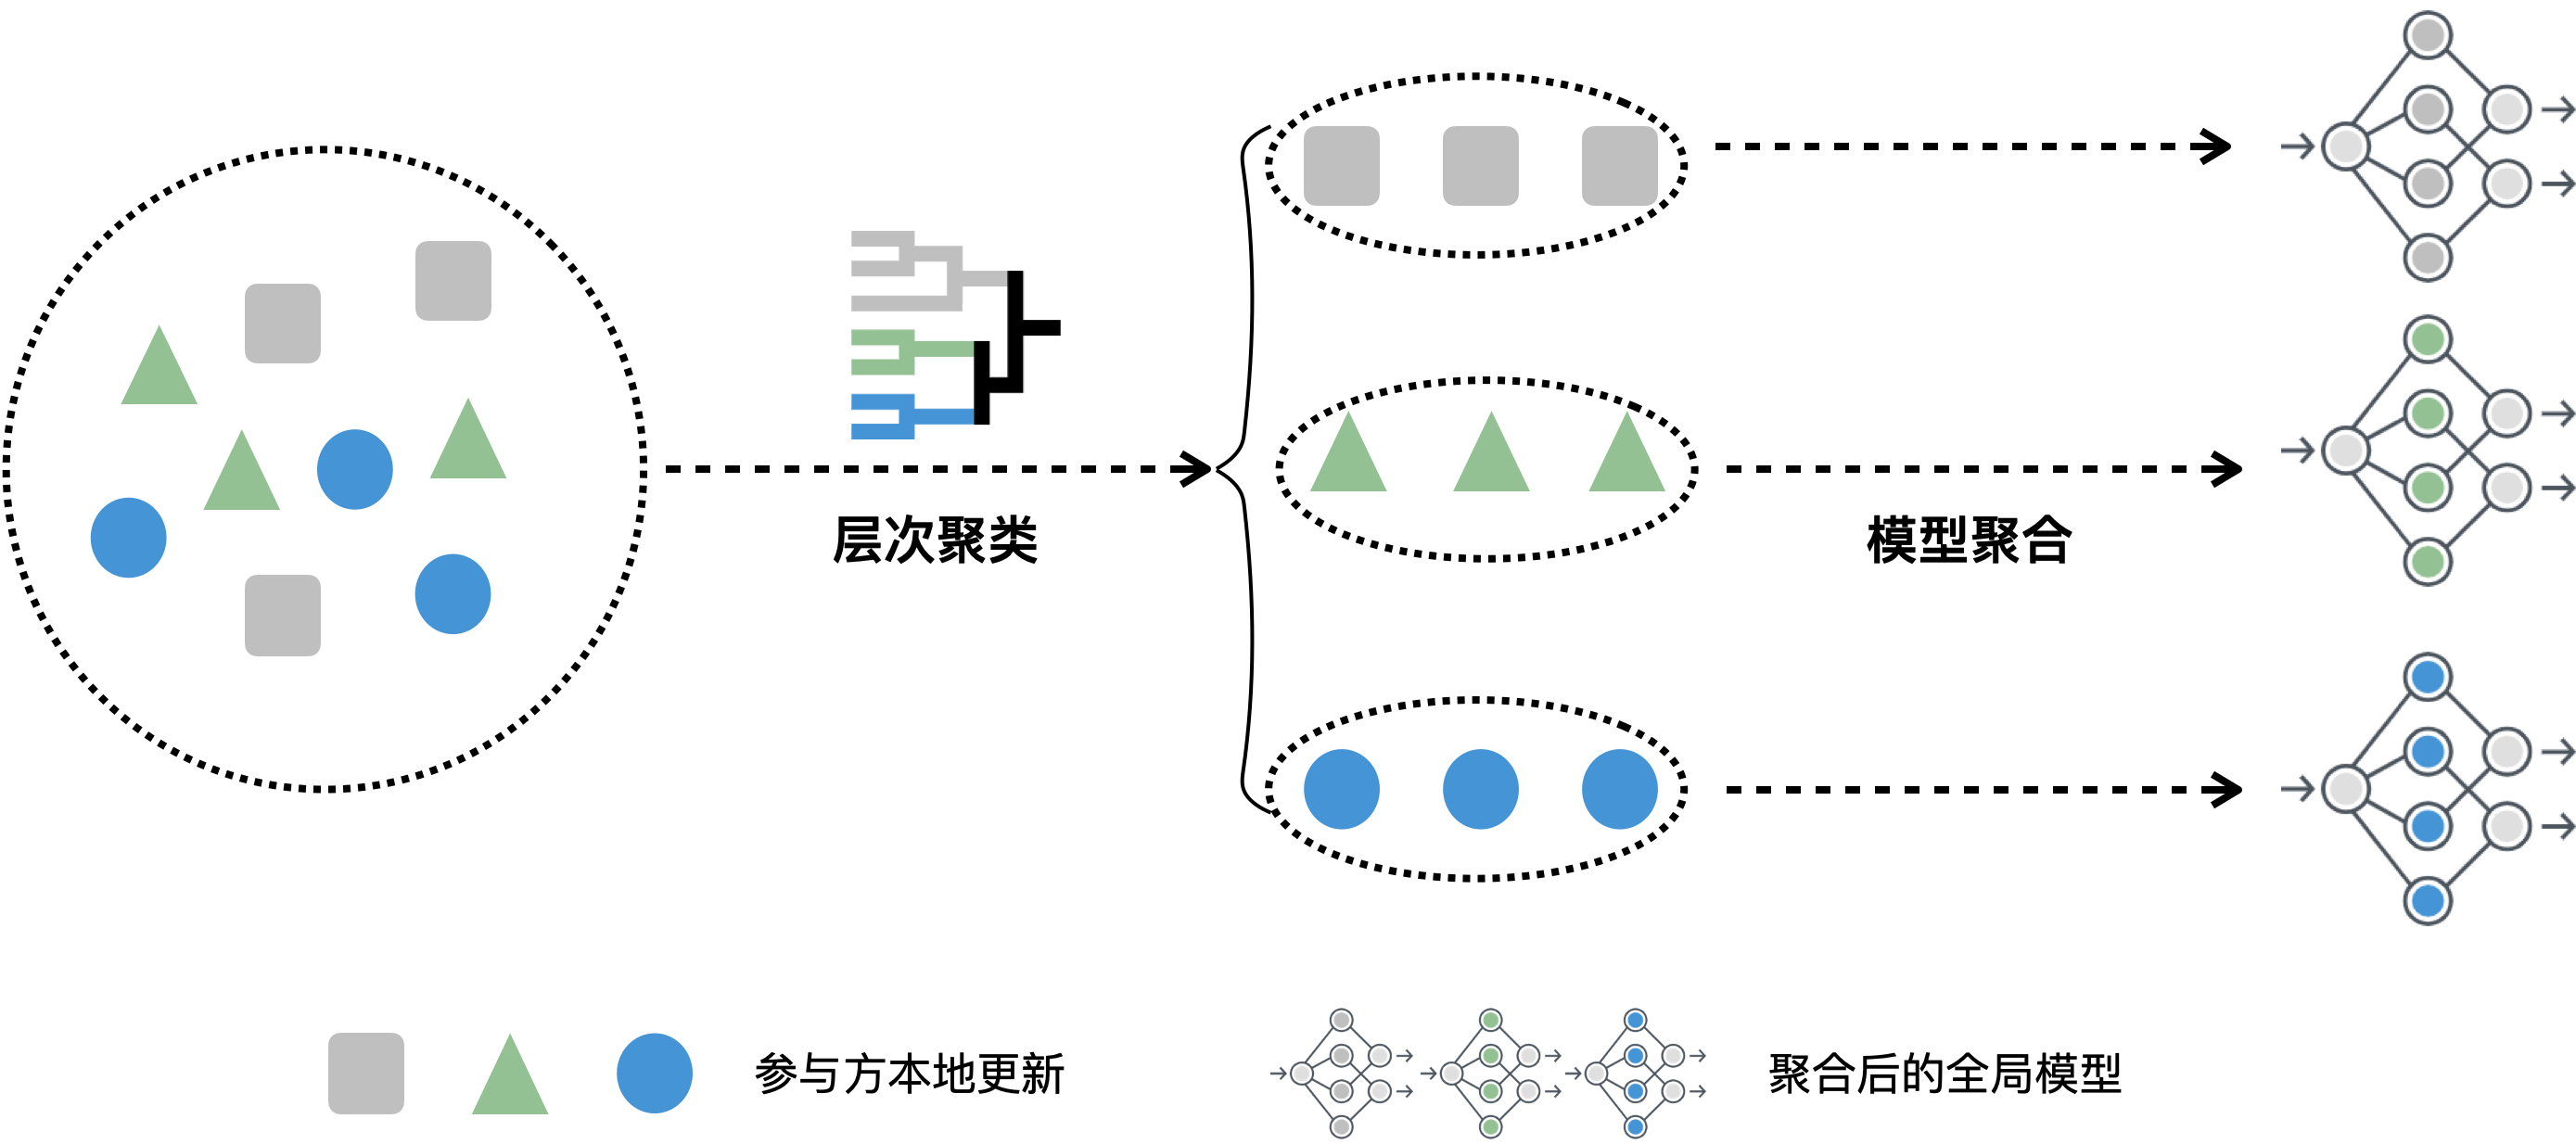
\includegraphics[width=0.8\linewidth]{FL+HC}
        \caption{FL+HC简介}
        \label{hcjpg}
    \end{center}
\end{figure}

\subsection{聚类分析指标}
PPFL+HC用于评估聚类结果的指标是调整Rand系数(Adjusted Rand Index,ARI)\cite{hubert1985comparing},它是对Rand系数(Rand Index,RI)\cite{rand1971objective}的修正。

Rand系数对比不同聚类算法的分类预测结果,统计两份结果中同属一个簇的点对与不同属一个簇的点对,将两者之和与全部点对的比作为指标,以此衡量两份预测结果之间的一致性。
具体而言,首先给出对同一份数据的两份聚类结果:$X = \{c_1, c_2,...,c_l\}$ 和 $Y = \{c_1,c_2, ...,c_k\}$,对于从数据集$\mathcal{D}$中获取的点对$(d_i, d_j)$,可以划分为如表\ref{ri-intro}所示的四类:
\begin{table}[!h]
	\centering
	\caption{点对$(d_i, d_j)$分类}
	\label{ri-intro}
	\begin{tabular}{c|c|c}
		\toprule
		是否在$X$中同属某簇 & 是否在$Y$中同属某簇 & 点对数量 \\
		\midrule
		\ding{51} & \ding{51} & $a$ \\
		\ding{55} & \ding{55} & $b$\\
		\ding{51} & \ding{55} & $c$ \\
		\ding{55} & \ding{51} & $d$\\
		\bottomrule
	\end{tabular}
\end{table}

Rand系数根据这四类点对数量的和$a,b,c,d$,按照等式\ref{ri-eq}计算得到指标,其中$n$表示数据集中元素的数量。
\begin{equation}\label{ri-eq}
	R=\frac{a+b}{a+b+c+d}=\frac{a+b}{{n \choose 2}}
\end{equation}

Rand系数取值为$[0,1]$,它无法对完全随机的结果保证接近与0,同时也没有负数的取值。针对以上问题,ARI利用统计方法将取值调整到$[-1,1]$,计算方式如等式\ref{ari-eq}所示。
\begin{equation}\label{ari-eq}
	A R I=\frac{R I-\mathbb{E}(R I)}{\max (R I)-\mathbb{E}(R I)}
\end{equation}
\subsection{密码技术介绍}

\subsubsection{加性秘密共享}
加性秘密共享是Shamir \cite{shamir1979share} 提出的一种安全多方计算技术。本章使用的是一种(2,2)的加性秘密共享方案,可用于安全两方计算(2PC)。这种方案可以在不同大小的环上做两方的安全计算,PPFL+HC使用到的是两种特殊的环,环$\mathbb{Z}_2$和$\mathbb{Z}_p, p=2^l$($l$一般为32)。当使用环$\mathbb{Z}_2$时,也被称为布尔秘密共享。
在布尔秘密共享方案中,布尔值$x \in \mathbb{Z}_2$可以被拆分为布尔共享份$\langle x\rangle_0^B$ 和 $\langle x\rangle_1^B$,其中三者满足$x = \langle x\rangle_0^B \oplus \langle x\rangle_0^B\;\text{mod}\;2$。
在使用环$x \in \mathbb{Z}_p$时,可以把环$\mathbb{Z}_p$上的元素$x$拆分为两个共享份$(\langle x\rangle_0, \langle x\rangle_1) = (r, x -r) \in \mathbb{Z}_p^2$, 其中$r$是在环$\mathbb{Z}_p$上均匀采样得到的元素。通过执行安全的两方计算协议 \cite{rathee2020cryptflow2, rathee2021sirnn},在不重构出原始值的情况下,完成任意的算术运算。

\subsubsection{本章使用的安全两方计算(2PC)协议}
为了在共享份额上进行进行安全的计算,本章使用了三种加性秘密共享上的基本运算 \cite{rathee2021sirnn},其基本信息描述如下:
\begin{compactitem}
    \item \textbf{安全两方有符号数乘法}(Signed Value Multiplication,$\mathcal{F}_{\text{SMul}}$): 有符号数乘法 $(\mathcal{F}_{\text{SMul}})$ 以两方上的共享份额 $\langle x\rangle$ 以及 $\langle y\rangle$ 作为输入,然后输出 $\langle z\rangle$,其中三者满足:$z = x \times y$。
    \item \textbf{安全两方多路选择器}(Multiplexer,$\mathcal{F}_{\text{MUX}}$): 多路选择器 $(\mathcal{F}_{\text{MUX}})$ 以 $\langle x\rangle^B$ 和 $\langle y\rangle$ 作为输入,然后输出 $\langle z\rangle$,其中如果$x = 1$,则输出的$z$满足$z = y$,否则满足$z = 0$。 
    \item \textbf{安全两方DRelu} $(\mathcal{F}_{\text{DRelu}})$: DRelu 函数 $(\mathcal{F}_{\text{DRelu}})$ 以 $\langle x\rangle$ 作为输入,然后输出 $\langle z\rangle^B$,其中如果$x \geq 0$,则输出的$z$满足 $z = 1$,否则满足 $z = 0$。
\end{compactitem}

\subsubsection{伪随机生成技术}
伪随机生成技术(Pseudorandom Generator, PRG)\cite{yao1982theory} 可以根据一个均匀分布的随机数种子,生成一串很长的伪随机字符。只要这个随机数种子不被敌对方窃取,就能保证生成的这段随机字符,无法在多项式时间内与均匀分布采样出来的字符串做出区分。本章方案在参数上传和分发阶段利用PRG技术在保证参数隐私的同时减少了一半的通信开销(细节见第\ref{4-framework}节)。

\section{问题描述}\label{4-problem}
本节主要对本章提出的PPFL+HC方案的系统模型、威胁模型以及设计目标,进行展开描述。

\subsection{系统模型}
本章设计的针对异质分布数据的隐私保护联邦学习方案PPFL+HC的系统模型如图\ref{sysjpg}所示。图中有$n$个参与方$P_1,P_2,...,P_n$和两个不共谋的服务器(联邦学习服务提供商(SP)和计算服务器(CS)),这种实体分布在相似的研究\cite{liu2021privacy, dong2021flod, hao2021efficient}中非常常见。SP主导整个联合学习过程,而CS在必要的时机协助SP完成秘密共享份额上的安全两方计算(2PC),每个参与方$P$拥有用于联合训练的本地数据集$D$(用户间的数据分布是异质的),每个参与方的目标是联合与其有着相似优化方向的其它参与方(即数据分布一致),训练得到性能更优的全局模型。PPFL+HC主要有以下三个步骤:
\begin{compactenum}
    \item SP将本轮全局模型参数广播给对应的用户。
    \item 每个参与方$P$将收到的全局模型参数应用到本地,然后利用本地数据$D$来更新模型参数,最后将更新梯度加密后发送给SP。
    \item 最后SP联合CS在特定轮次对梯度进行层次聚类,根据层次聚类结果对共享后的梯度进行安全的聚合。
\end{compactenum}


\begin{figure}[htbp]
    \begin{center}
        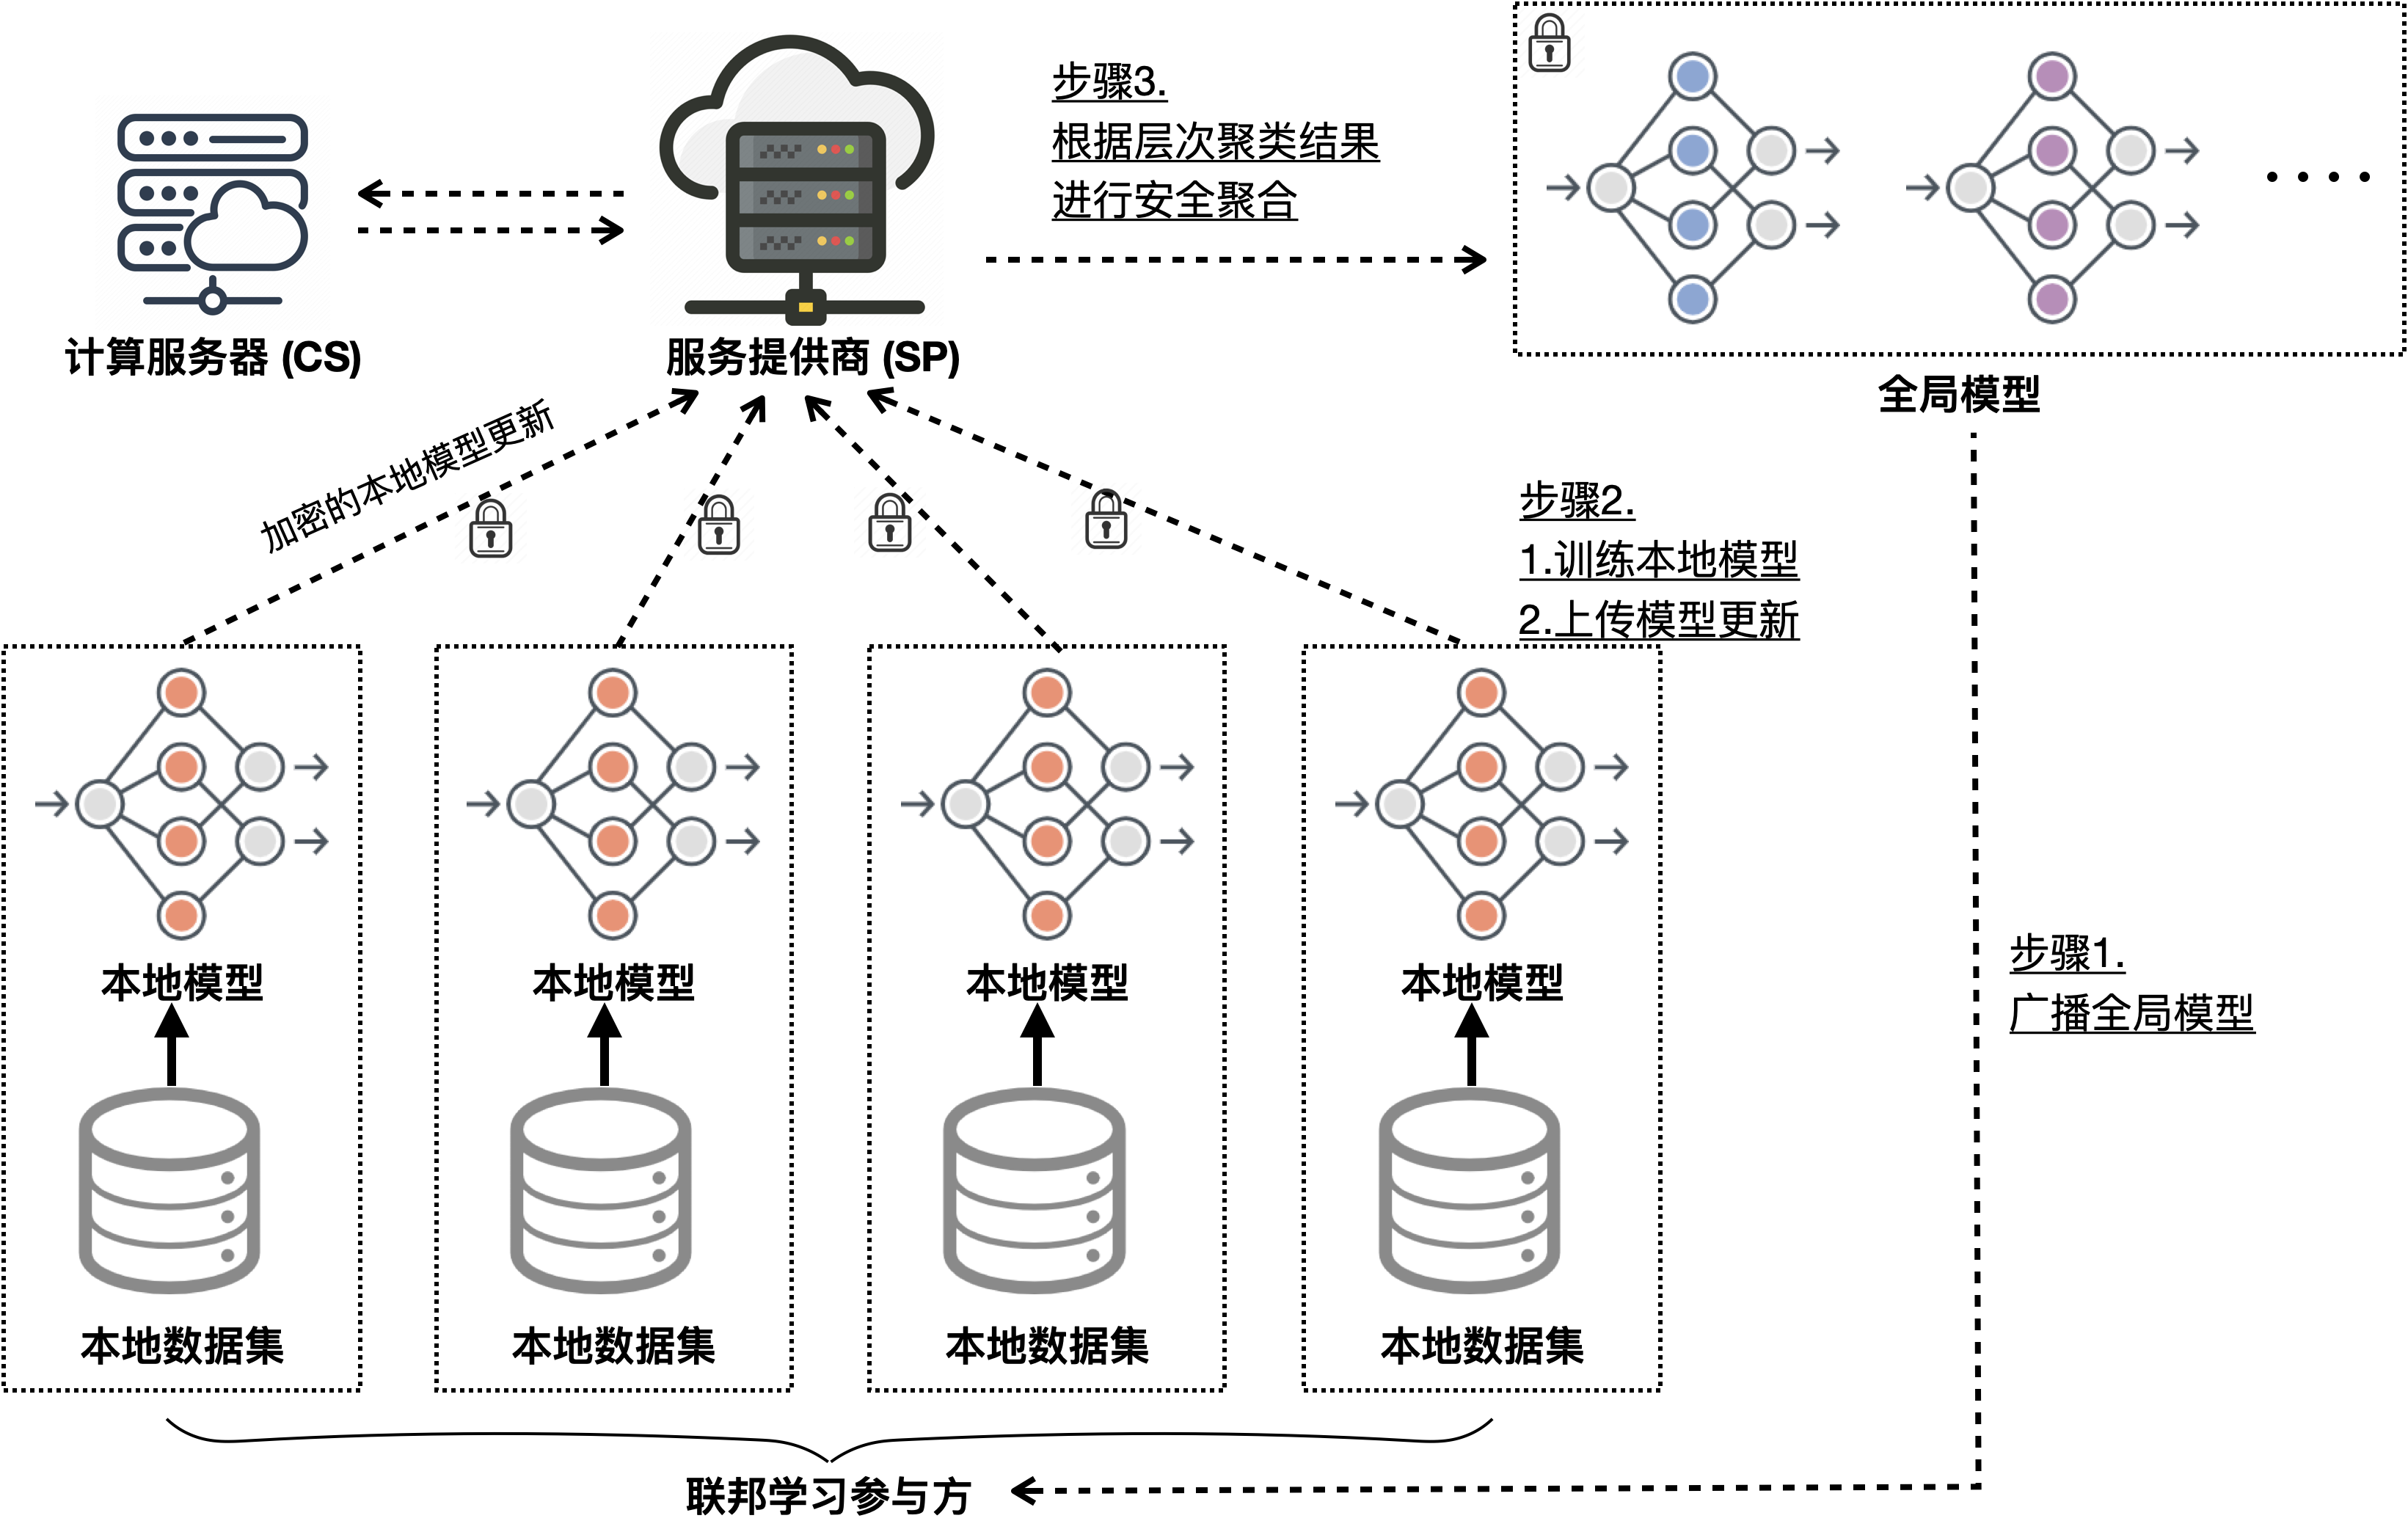
\includegraphics[width=0.8\columnwidth]{PPFL-HC}
        \caption{PPFL+HC系统模型图}
        \label{sysjpg}
    \end{center}
\end{figure}

\subsection{威胁模型}
本章方案PPFL+HC将服务器(SP和CS)视为诚实且好奇的,这意味着SP和CS将严格执行本章设计的安全协议,但会主动尝试推断用户的隐私信息。除此之外,PPFL+HC还假设,SP和CS因为害怕公信力的丧失,不会发生共谋行为,这可以保证PPFL+HC按照(2,2)加性秘密共享上传的用户模型参数不会泄露给服务器。这个威胁模型可以在真实世界中满足,并且在类似工作\cite{nguyen2022flame}中也用到了同样的威胁模型。举例来说,Google和Amazon两种服务提供商,为了维护自己的信誉,都会选择正确执行本章设计的安全协议,而不是共谋获取用户的隐私信息。

\subsection{设计目标}
本章的目标是在保证用户梯度隐私的同时,提升联邦学习在面对异质分布数据的联合训练性能。具体来说,设计目标如下:
\begin{compactitem}
    \item \textbf{梯度隐私保护:}本章致力于实现对梯度的强隐私保护,其中包括对用户上传的本地梯度的隐私保护,以及聚合之后的全局梯度的隐私保护。
    \item \textbf{异质分布数据准确率提升:}本章通过实现对梯度共享份上的安全层次聚类,来提升联邦学习在面对异质分布数据的联合训练性能下降问题。
    \item \textbf{高效的安全计算协议:}本章精心设计了2PC协议,保证在聚类以及聚合结果正确性的同时,尽量减小计算和通信的复杂度。
\end{compactitem}

\section{基于秘密共享的隐私保护计算模块}\label{4-building}
%介绍为什么要设计这几个模块
为了对$n$个参与方的梯度向量的共享份$\{\boldsymbol{\langle g_1\rangle}, \boldsymbol{\langle g_2\rangle},...,\boldsymbol{\langle g_n\rangle} \}$进行安全的层次聚类操作,最首要的工作就是度量梯度向量之间的相似性,在层次聚类中,度量方式有欧式距离、曼哈顿距离以及余弦相似度,鉴于余弦相似度计算涉及到的开方和除法在共享份上的计算开销较大,本章仅考虑安全的欧式距离计算和安全的曼哈顿距离计算,并基于安全的距离度量方式提出了安全层次聚类算法。

为了更好的描述提出的安全算法,表\ref{table-sym}对本章使用到的符号进行了梳理,其中$\langle \cdot\rangle$表示变量的共享份,下标为0的变量$\langle \cdot\rangle_0$表示SP持有的共享份,下标为1的变量$\langle \cdot\rangle_1$表示CS持有的共享份。具体描述见表\ref{table-sym}。

\begin{table}
	\centering
	\caption{符号说明}
	\label{table-sym}
	\scalebox{1.0}{
		\renewcommand{\arraystretch}{1.2}
		\begin{tabular}{cl}
			\toprule
			\textbf{符号}               & \textbf{描述}                      \\
			\midrule
			$\boldsymbol{g_i}$                          & 参与方 $P_i$ 的本地梯度向量      \\
			$\boldsymbol{G_x}$                          & 聚类结果中簇 $c_x$ 的全局梯度向量     \\
			$\boldsymbol{\langle g_i\rangle}$           & $\boldsymbol{g_i}$ 的共享份,其中 \\
			& SP 持有 $\boldsymbol{\langle g_i\rangle_0}$,CS 持有$\boldsymbol{\langle g_i\rangle_1}$ \\
			$\mathcal{D}_i$                & 参与方 $P_i$ 的本地数据集             \\
			$\textit{EDis}$                & 欧式距离(Euclidean distance)                        \\ 
			$\textit{MDis}$                & 曼哈顿距离(Manhattan distance)                        \\
			\bottomrule
		\end{tabular}
	}
\end{table}

\subsection{安全欧式距离计算}
为了安全的计算共享梯度向量$\boldsymbol{\langle g_i\rangle}$和$\boldsymbol{\langle g_j\rangle}$之间的欧式距离$\Vert \boldsymbol{g_i} - \boldsymbol{g_j} \Vert_2$,本章设计了安全的欧式距离(Secure Euclidean Distance, SED)计算算法。
首先SP和CS在本地计算$\boldsymbol{\langle z\rangle} = \boldsymbol{\langle g_i\rangle} - \boldsymbol{\langle g_j\rangle}$,然后SP和CS对于两个向量中的每一个元素协同调用$\mathcal{F}_{\text {SMul}}$,其中SP的输入是$\boldsymbol{\langle z\rangle_0}[i]$,CS的输入是$\boldsymbol{\langle z\rangle_1}[i]$,然后SP和CS得到乘法的计算结果的共享份$\boldsymbol{\langle d\rangle}[i]$。
接下来SP和CS在本地计算向量$\boldsymbol{\langle d\rangle}$所有元素的内部和$\sum_{i=1}^{m} \boldsymbol{\langle d\rangle}[i]$,得到欧式距离平方的共享份$\langle \textit{EDis}^2\rangle$。
最后CS将共享份额$\langle \textit{EDis}^2\rangle_1$发送给SP,SP完成重构得到欧式距离明文$\textit{EDis}$(这个解密行为不会侵犯用户数据隐私,见第\ref{smd}节中的讨论)。
通过运行SED,SP和CS可以在不泄漏$\boldsymbol{g_i}$和$\boldsymbol{g_j}$每一个元素的情况下,得到梯度之间的欧式距离$\textit{EDis}$。SED算法的细节描述如算法\ref{alg1}所示。

\begin{algorithm}[htbp]
    \caption{安全欧式距离计算\\$\text{SED}(\boldsymbol{\langle g_i\rangle}, \boldsymbol{\langle g_j\rangle}) \xrightarrow{} \textit{EDis}$}
    \label{alg1}
    % \renewcommand{\algorithmicrequire}{\textbf{Input:}}
    % \renewcommand{\algorithmicensure}{\textbf{Output:}}
    \begin{algorithmic}[1]
    \REQUIRE SP拥有$\boldsymbol{\langle g_i\rangle_0}$和$\boldsymbol{\langle g_j\rangle_0}$, CS拥有$\boldsymbol{\langle g_i\rangle_1}$和$\boldsymbol{\langle g_j\rangle_1}$。 $\mathcal{F}_{\text {SMul}}$在文献\cite{rathee2021sirnn}中提出。
    \ENSURE $\boldsymbol{g_i}$和$\boldsymbol{g_j}$之间的欧式距离$\textit{EDis}$。
    % content
    \STATE SP本地计算$\boldsymbol{\langle z\rangle_0} = \boldsymbol{\langle g_i\rangle_0} - \boldsymbol{\langle g_j\rangle_0}$
    \STATE CS本地计算$\boldsymbol{\langle z\rangle_1} = \boldsymbol{\langle g_i\rangle_1} - \boldsymbol{\langle g_j\rangle_1}$
    % \STATE $\mathcal{F}_{\text {SMul }}(\langle z\rangle, \langle z\rangle)$
%    \FOR[$m$是$\boldsymbol{g_i}$的维度]{$i \in 1\:\textbf{to}\:m$} %\COMMENT{$m$ is the dimension of $\boldsymbol{g_i}$}
%        \STATE SP和CS调用函数$\mathcal{F}_{\text {SMul}}$, 其中SP的输入是$\boldsymbol{\langle z\rangle_0}[i]$,而CS的输入是 $\boldsymbol{\langle z\rangle_1}[i]$. 运算结束后SP和CS分别得到乘法结果的共享份$\boldsymbol{\langle d\rangle_0}[i]$ 和 $\boldsymbol{\langle d\rangle_1}[i]$。
%        % \STATE $(\lrangle EDis[i]\rangle,angle EDis[i]\rangle = \mathcal{F}_{\text {SMul }}(\langle z\rangle[i], \langle z\rangle[i])$
%    \ENDFOR
    \STATE SP和CS调用函数$\mathcal{F}_{\text {SMul}}$,其中两个乘数都是SP和CS持有的共享份$\boldsymbol{\langle z\rangle}$,计算得到乘法结果的共享份$\boldsymbol{\langle d\rangle}$ \COMMENT{对向量$\boldsymbol{\langle z\rangle}$中的元素逐个调用$\mathcal{F}_{\text {SMul}}$}
    \STATE SP本地计算$\langle \textit{EDis}^2\rangle_0 = \sum_{i=1}^{m} \boldsymbol{\langle d\rangle_0}[i]$
    \STATE CS本地计算$\langle \textit{EDis}^2\rangle_1 = \sum_{i=1}^{m} \boldsymbol{\langle d\rangle_1}[i]$
    \STATE CS发送$\langle \textit{EDis}^2\rangle_1$给SP, SP重构$\textit{EDis}^2 = \langle \textit{EDis}^2\rangle_0 + \langle \textit{EDis}^2\rangle_1$然后开方得到$\textit{EDis}$。
    \RETURN SP得到欧氏距离$\textit{EDis}$。
    \end{algorithmic}
\end{algorithm}

\subsection{安全曼哈顿距离计算}\label{smd}
为了安全的计算共享梯度向量$\boldsymbol{\langle g_i\rangle}$和$\boldsymbol{\langle g_j\rangle}$之间的曼哈顿距离$\norm{\boldsymbol{g_i} - \boldsymbol{g_j}}_1$,本章设计了安全的曼哈顿距离(Secure Manhattan Distance, SMD)计算算法。
首先SP和CS在本地计算$\boldsymbol{\langle z\rangle} = \boldsymbol{\langle g_i\rangle} - \boldsymbol{\langle g_j\rangle}$,然后SP联合CS以共享份$\boldsymbol{\langle z\rangle}$为输入,调用函数$\mathcal{F}_{\text {SMul}}$,计算得到DRelu值的布尔共享份$\boldsymbol{\langle y\rangle}^{B}$。
接着SP和CS分别计算$\boldsymbol{\langle \widetilde{y} \rangle_0}^{B} = \boldsymbol{\langle y\rangle_0}^{B}$和$\boldsymbol{\langle \widetilde{y} \rangle_1}^{B} = \boldsymbol{\langle y\rangle_1}^{B} \oplus 1$,得到DRelu结果对应的布尔取反结果$\boldsymbol{\langle \widetilde{y} \rangle}^{B}$。
紧接着SP和CS调用两次安全多路选择器,分别以$\{\boldsymbol{\langle z\rangle}, \boldsymbol{\langle y\rangle}^{B}\}$、$\{\boldsymbol{\langle z\rangle}, \boldsymbol{\langle \widetilde{y}\rangle}^{B}\}$为输入,获取$\boldsymbol{\langle z\rangle}$中的正数集合$\boldsymbol{
	\langle d_p\rangle}$以及负数集合$\boldsymbol{
	\langle d_n\rangle}$。
最后SP和CS在本地计算$\langle \textit{MDis}\rangle = \sum_{i=1}^{m}\boldsymbol{\langle d_p\rangle}[i] - \sum_{i=1}^{m}\boldsymbol{\langle d_n\rangle}[i]$,CS将结果共享份$\langle \textit{MDis}\rangle_1$发送给SP,SP完成重构得到曼哈顿距离$\textit{MDis}$。
SMD具体的算法细节描述如算法\ref{alg2}所示。

\textbf{讨论:}在本章的安全欧式距离以及安全的曼哈顿距离计算中,都将最后的结果($\langle \textit{EDis}\rangle$和$\langle \textit{MDis}\rangle$)从共享份重构为明文($\textit{EDis}$和$\textit{MDis}$),本章认为这个距离信息的重构不会侵犯用户的数据隐私,
%很明显即使SP能够得到任意两个梯度之间的距离信息,也无法推断出任何一个梯度的具体信息,包括梯度的大小、方向以及单个元素的正负。文献\cite{geiping2020inverting}提出的针对梯度的数据重构方案,可以根据梯度之间的余弦相似度,重构用户的训练样本,但是这个方案需要知道梯度的正负,而在本章的方案中,SP是无法获取这个信息的,所以不会泄露用户的数据隐私。
理由与第\ref{broadcast-para}节末尾的讨论类似。首先,PPFL+HC实现了全局模型参数对SP和CS的保密(细节见第\ref{distribution}节),SP无法根据全局模型生成虚拟的梯度信息。其次,SP获取的这一轮次两两梯度之间的距离信息,无法据此推断出任何一份梯度的具体信息,包括梯度的大小、方向以及单个元素的正负,SP不能根据真实梯度构造优化目标。综上,距离信息的重构不会侵犯用户的数据隐私。

\begin{algorithm}[htbp]
    \caption{安全曼哈顿距离计算\\$\text{SMD}(\boldsymbol{\langle g_i\rangle}, \boldsymbol{\langle g_j\rangle}) \xrightarrow{} \textit{MDis}$}
    \label{alg2}
    \begin{algorithmic}[1]
    % \renewcommand{\algorithmicrequire}{\textbf{Input:}}
    % \renewcommand{\algorithmicensure}{\textbf{Output:}}
    \REQUIRE SP 拥有 $\boldsymbol{\langle g_i\rangle_0}$ 和 $\boldsymbol{\langle g_j\rangle_0}$, CS 拥有 $\boldsymbol{\langle g_i\rangle_1}$ 和 $\boldsymbol{\langle g_j\rangle_1}$. $\mathcal{F}_{\text {DRelu}}$ 和 $\mathcal{F}_{\text {MUX}}$ 在文献\cite{rathee2021sirnn}中提出。
    \ENSURE $\boldsymbol{g_i}$ 与 $\boldsymbol{g_j}$之间的曼哈顿距离$\textit{MDis}$。
    % content
    \STATE SP 本地计算 $\boldsymbol{\langle z\rangle_0} = \boldsymbol{\langle g_i\rangle_0} - \boldsymbol{\langle g_j\rangle_0}$
    \STATE CS 本地计算 $\boldsymbol{\langle z\rangle_1} = \boldsymbol{\langle g_i\rangle_1} - \boldsymbol{\langle g_j\rangle_1}$
    \STATE SP 和 CS 调用 $\mathcal{F}_{\text{DRelu}}$,其中输入为SP和CS持有的共享份$\boldsymbol{\langle z\rangle}$,计算得到DRelu值的布尔共享份$\boldsymbol{\langle y\rangle}^{B}$。
    \STATE SP 和 CS 分别调用 $\boldsymbol{\langle \widetilde{y} \rangle_0}^{B} = \boldsymbol{\langle y\rangle_0}^{B}$ 和 $\boldsymbol{\langle \widetilde{y} \rangle_1}^{B} = \boldsymbol{\langle y\rangle_1}^{B} \oplus 1$。\COMMENT{安全的获得布尔共享份$\boldsymbol{\langle y\rangle}^{B}$的取反结果$\boldsymbol{\langle \widetilde{y} \rangle}^{B}$。}
    % \State SP sets $\boldsymbol{\langle \widetilde{g_i}\rangle_0}$ = - $\boldsymbol{\langle g_i\rangle_0}$ and $\boldsymbol{\langle \widetilde{g_j}\rangle_0}$ = - $\boldsymbol{\langle g_j\rangle_0}$
    % \State CS sets $\boldsymbol{\langle \widetilde{g_i}\rangle_1}$ = - $\boldsymbol{\langle g_i\rangle_1}$ and $\boldsymbol{\langle \widetilde{g_j}\rangle_1}$ = - $\boldsymbol{\langle g_j\rangle_1}$
    % \For{$i \in [1...m]$} \Comment{$m$ is the dimension of $\boldsymbol{g_i}$}
        \STATE SP 和 CS 调用 $\mathcal{F}_{\text{MUX}}$,其中输入为SP和CS持有的共享份$\boldsymbol{\langle z\rangle}$ 和 $\boldsymbol{\langle y\rangle}^{B}$,计算得到$\boldsymbol{\langle z\rangle}$中的正数集合$\boldsymbol{
        \langle d_p\rangle}$。
        \STATE SP 和 CS 调用 $\mathcal{F}_{\text{MUX}}$,其中输入为SP和CS持有的共享份 $\boldsymbol{\langle z\rangle}$ 和 $\boldsymbol{\langle \widetilde{y}\rangle}^{B}$,计算得到$\boldsymbol{\langle z\rangle}$中的负数集合$\boldsymbol{
        \langle d_n\rangle}$
    % \EndFor
    \STATE SP 本地计算 $\langle \textit{MDis}\rangle_0 = \sum_{i=1}^{m}\boldsymbol{\langle d_p\rangle_0}[i] - \sum_{i=1}^{m}\boldsymbol{\langle d_n\rangle_0}[i]$ \COMMENT{$m$ 是 $\boldsymbol{g_i}$的维度}
    \STATE CS 本地计算 $\langle \textit{MDis}\rangle_1 = \sum_{i=1}^{m}\boldsymbol{\langle d_p\rangle_1}[i] - \sum_{i=1}^{m}\boldsymbol{\langle d_n\rangle_1}[i]$
    \STATE CS 发送 $\langle \textit{MDis}\rangle_1$ 给 SP,然后SP 重构出 $\textit{MDis} = \langle \textit{MDis}\rangle_0 + \langle \textit{MDis}\rangle_1$。
    \RETURN SP得到曼哈顿距离$\textit{MDis}$。
    \end{algorithmic}
\end{algorithm}

\subsection{安全梯度层次聚类}
%写随机梯度裁剪
为了完成对共享份梯度集合$\{\boldsymbol{\langle g_1\rangle}, \boldsymbol{\langle g_2\rangle},...,\boldsymbol{\langle g_n\rangle} \}$的安全层次聚类,本章将整个聚类过程划分为三个阶段:
\begin{compactenum}
	\item \textbf{梯度的随机降维:}考虑到神经网络梯度的维度较高,而对梯度的层次聚类不使用全部维度也能保证较高的准确性(实验验证参考第\ref{hc-test}节),本章对梯度进行了随机降维操作,随机抽取一部分元素,对所有的梯度向量 $\{\boldsymbol{\langle g_1\rangle}, \boldsymbol{\langle g_2\rangle},...,\boldsymbol{\langle g_n\rangle} \}$ 抽取相同下标的一部分元素,得到降维后的梯度向量 $\{\dot{\boldsymbol{\langle g_1\rangle}}, \dot{\boldsymbol{\langle g_2\rangle}},...,\dot{\boldsymbol{\langle g_n\rangle}} \}$。
	\item \textbf{梯度间距离矩阵计算:}这一阶段完成每个共享梯度向量$\dot{\svec{g_i}}$,与其它$n-1$个梯度的距离计算,得到一个距离矩阵:
	\[
	\begin{bmatrix}
		\textit{Dis}_{1,1} & \textit{Dis}_{1,2} & \cdots & \textit{Dis}_{1,n} \\
		\textit{Dis}_{2,1} & \textit{Dis}_{2,2} & \cdots & \textit{Dis}_{2,n} \\
		\vdots & \vdots & \ddots & \vdots \\
		\textit{Dis}_{n,1} & \textit{Dis}_{n,2} & \cdots & \textit{Dis}_{n,n}
	\end{bmatrix}
	\]
%	$$\{\textit{Dis}_{11}, \textit{Dis}_{12},...,\textit{Dis}_{1n};\textit{Dis}_{21}, \textit{Dis}_{22},...,\textit{Dis}_{2n};...;\textit{Dis}_{n1}, \textit{Dis}_{n2},...,\textit{Dis}_{nn}\},$$
	其中距离的计算过程以梯度共享份为输入,调用上述SED或SMD安全距离计算算法,在保证梯度隐私的前提下,得到明文的距离矩阵。
	\item \textbf{基于距离矩阵的聚类过程:}在得到预先计算好的距离矩阵之后,再搭配其它层次聚类参数,比如不同的簇间距离计算方式(Average,Complete,Ward等)以及距离阈值,完成对梯度的自底向上的层次聚类。
\end{compactenum}
具体的安全层次聚类算法细节如算法\ref{alg3}所示。

\begin{algorithm}[htbp]
	\caption{安全的梯度层次聚类算法 \\ $\text{SHC}(\{\boldsymbol{\langle g_1\rangle}, \boldsymbol{\langle g_2\rangle},...,\boldsymbol{\langle g_n\rangle} \}) \rightarrow \{c_1,c_2,...,c_l \}$}
	\label{alg3}
	\begin{algorithmic}[1]
		\REQUIRE SP 和 CS 拥有$\{\boldsymbol{\langle g_1\rangle}, \boldsymbol{\langle g_2\rangle},...,\boldsymbol{\langle g_n\rangle} \}$。 \COMMENT{$n$ 表示参与方数量}
		\ENSURE $l$ 个簇 $\{c_1,c_2,...,c_l \}$。
		% content
		\STATE SP 和 CS 对梯度共享份 $\{\boldsymbol{\langle g_1\rangle}, \boldsymbol{\langle g_2\rangle},...,\boldsymbol{\langle g_n\rangle} \}$ 进行随机降维得到:\\ $\{\dot{\boldsymbol{\langle g_1\rangle}}, \dot{\boldsymbol{\langle g_2\rangle}},...,\dot{\boldsymbol{\langle g_n\rangle}} \}$
		\FOR{$i \gets 1\:\textbf{to}\:n$}
		\FOR{$j \gets 1\:\textbf{to}\:n$}
			\STATE SP 和 CS 调用$\textit{Dis}_{ij} \xleftarrow{}\text{SMD}(\dot{\boldsymbol{\langle g_i\rangle}}, \dot{\boldsymbol{\langle g_j\rangle}})$ (或者 $\text{SED}(\dot{\boldsymbol{\langle g_i\rangle}}, \dot{\boldsymbol{\langle g_j\rangle}})$), 然后SP获得距离值$\textit{Dis}_{ij}$。
		\ENDFOR
		\ENDFOR
%		\STATE $\{c_1,c_2,...,c_l \} \xleftarrow{} \textsc{Clustering}(\textit{Dis}_{11},...,\textit{Dis}_{nn})$ \COMMENT{基于预计算距离矩阵的明文层次聚类}
		\STATE $\{c_1,c_2,...,c_l \} \xleftarrow{} \textsc{Clustering}$(\(\begin{bmatrix}
			\textit{Dis}_{1,1} & \textit{Dis}_{1,2} & \cdots & \textit{Dis}_{1,n} \\
			\textit{Dis}_{2,1} & \textit{Dis}_{2,2} & \cdots & \textit{Dis}_{2,n} \\
			\vdots & \vdots & \ddots & \vdots \\
			\textit{Dis}_{n,1} & \textit{Dis}_{n,2} & \cdots & \textit{Dis}_{n,n}
		\end{bmatrix}\)) \COMMENT{基于预计算距离矩阵的明文层次聚类过程}
		\RETURN SP和CS获得层次聚类结果 $\{c_1,c_2,...,c_l \}$。
	\end{algorithmic}
\end{algorithm}


\section{面向异质分布数据的隐私保护联邦学习方案}\label{4-framework}
基于\ref{4-building}节设计的相关安全计算模块,本节介绍设计的面向异质分布数据的隐私保护联邦学习方案PPFL+HC,在FL+HC\cite{briggs2020federated}的基础上,PPFL+HC实现了对用户梯度和聚合后的全局梯度的强隐私保护。
本节首先介绍方案概述,然后具体阐述方案的四个阶段:初始化阶段、本地梯度的生成和编码阶段、梯度的安全聚和阶段以及聚合梯度的安全分发阶段。在整个方案中,用户上传的梯度信息以及聚合生成的全局梯度信息,都不会被SP以及CS窃取。
%实现了对梯度的完全隐私保护。

\subsection{方案概述}
参与方$P_i$在本地生成梯度之后,利用文献\cite{hao2021efficient}的方法,PPFL+HC仅向SP上传一份梯度共享份$\svec{g_i}$,另一份梯度共享份由$P_i$和CS利用相同的随机数种子(在初始化阶段协商),借助伪随机算法PRG生成,以此减少一半的通信开销。
在梯度的聚合阶段,SP和CS在聚类轮次执行一次安全的梯度层次聚类,然后根据聚类结果为每个簇单独聚合生成全局梯度,对于聚类轮次之前的轮次,所有的参与方被视为一个簇。
最后SP和CS完成对聚合梯度的安全分发,保证全局梯度的隐私。

\subsection{具体方案}
%本节具体介绍方案涉及到的四个阶段。
%TODO add frame flow.

\subsubsection{初始化阶段}
本阶段在整个方案中只会被执行一次。利用文献\cite{diffie2022new}提出的Diffie-Hellman密钥协商协议,每个参与方$P_i$与CS协商一个私有的种子密钥$k_i^{seed}$。这个密钥在本地梯度的上传以及全局梯度的分发过程中,保证参与方$P_i$与CS能够非交互的生成同样的随机向量,具体细节见阶段\ref{local}和阶段\ref{distribution}。

\subsubsection{本地梯度的生成和编码阶段}\label{local}
本阶段描述参与方$P_i$如何生成本地梯度的共享份$\svec{g_i}$,包括上传给SP的共享份$\svec[0]{g_i}$,以及与CS协同生成的共享份$\svec[1]{g_i}$。

首先,参与方$P_i$利用收到的全局梯度更新本地模型,再使用本地数据$\mathcal{D}_i$训练模型得到本地的原始参数更新,是一个浮点数梯度向量$\overline{\bs{g_i}}$。
为了将浮点梯度$\overline{\bs{g_i}}$表示为环 $\mathbb{Z}_p$($p=2^l$,$l$表示比特长度)上的共享份,首先要对这个向量进行定点数编码。
对于浮点数 $v$ 来说,本节使用的定点编码操作如下:
\begin{equation}
	Encode(v) = \lfloor 2^s \times v\rfloor \;\text{mod}\;p
\end{equation}
其中 $\lfloor v\rfloor$表示小于等于浮点数 $v$ 的最大整数值,而 $s$ 表示定点数的精度。
对浮点向量 $\overline{\bs{g_i}}$ 中的每个元素都进行定点编码,于是就得到了本地梯度的定点表示:
\begin{equation}
	\boldsymbol{g_i} = Encode(\overline{\boldsymbol{g_i}})
\end{equation}
然后参与方$P_i$使用PRG技术,利用随机数种子 $k_i^{seed}$生成随机向量 $\bs{r_i}$,然后将属于SP的梯度共享份 $\svec[0]{g_i} = \bs{g_i} - \bs{r_i}$ 发送给SP。为了提升通信效率,CS在本地使用同样的随机数种子 $k_i^{seed}$ 生成相同的随机变量 $\bs{r_i}$,所以属于CS的梯度共享份为 $\svec[1]{g_i} = \bs{r_i}$,这种方式减少了梯度上传过程中一半的通信开销。

\subsubsection{梯度的安全聚合阶段}
在PPFL+HC中,会在特定的轮次 $t$ 进行梯度的安全层次聚类操作,在轮次 $t$ 之前,所有的参与方被视为一个簇,联合生成一个全局梯度(与FedAvg \cite{mcmahan2017communication} 一致)。当进行到第$t$轮时,对所有的梯度执行安全的层次聚类操作:
\begin{equation}
	\{c_1,c_2,...,c_l \} \leftarrow \text{SHC}(\{\boldsymbol{\langle g_1\rangle}, \boldsymbol{\langle g_2\rangle},...,\boldsymbol{\langle g_n\rangle} \})
\end{equation}
得到聚类结果$\{c_1,c_2,...,c_l \}$后,对于一个簇中的所有参与方,进行线性聚合操作:
\begin{equation}
	\boldsymbol{\langle G_x\rangle} = \frac{\sum_{j \in c_x}\boldsymbol{\langle g_j\rangle}}{n_x}
\end{equation}
其中$j$ 表示簇 $c_x$ 中的参与方,$n_x$ 表示簇 $c_x$ 中参与方的数量,$\svec{G_x}$ 表示聚合之后的全局梯度,以此得到所有的聚合全局梯度的共享份 $\{\svec{G_1},\svec{G_2},...,\svec{G_l}\}$。


\subsubsection{梯度的安全广播阶段}\label{distribution} 
为了保证全局梯度 $\svec{G_x}$ 的隐私,PPFL+HC没有选择让SP和CS重构出$\bs{G_x}$再广播给用户。而是设计了安全的参数分发算法,在不提升通信开销的同时,保证了全局梯度的隐私,算法细节描述如算法\ref{alg4}所示。首先参与方$P_i$ 和 CS利用$k_i^{seed}$协同生成相同的随机变量$\bs{r_i^{\prime}}$,然后CS使用该随机变量对梯度共享份进行扰动得到 $\svec[0]{\widehat{G_x}} = \svec[0]{G_x} + \bs{r_i^{\prime}}$,紧接着CS将 $\svec[0]{\widehat{G_x}}$ 发送给SP,SP重构扰动之后的全局梯度 $\boldsymbol{\widehat{G_x}} = \boldsymbol{\langle G_x\rangle_0} + \boldsymbol{\langle \widehat{G_x}\rangle_1}$,最后将 $\boldsymbol{\widehat{G_x}}$ 发送给参与方$P_i$,$P_i$利用$r_i^{\prime}$消除扰动得到$\boldsymbol{G_x}$。

参与方$P_i$拿到全局梯度$\bs{G_x}$后,对梯度进行定点数解码操作:
\begin{equation}
	\bs{\overline{G_x}} = Decode(\bs{G_x})
\end{equation}
其中解码操作首先将元素$v$视为浮点数,然后除以$2^s$,得到对应的梯度浮点数。

\begin{algorithm}[htbp]
	\caption{安全的全局梯度广播 \\$\text{SGB}(\boldsymbol{\langle G_x\rangle}) \rightarrow \boldsymbol{G_x}$}
	\label{alg4}
	\begin{algorithmic}[1]
		\REQUIRE SP 和 CS 拥有参与方 $P_i$的全局梯度$\boldsymbol{\langle G_x\rangle}$.
		% clustering results $\{c_1,c_2,...,c_l\}$ and global gradients $\{\boldsymbol{\langle G_1\rangle,...,\langle G_l\rangle\}}$ \Comment{$l$ is the number of clusters}
		\ENSURE 参与方$P_i$ 获得相应的全局梯度$\boldsymbol{G_x}$
		% \Comment{$x$ indicates the cluster to which $P_i$ belongs}
		% content
		\STATE $P_i$ 与 CS 利用相同的随机数种子生成 $\boldsymbol{r_i}$ = PRG($k_i^{seed}$) \COMMENT{相同的$k_i^{seed}$ 保证了$\boldsymbol{r_i}$ 在 $P_i$ 和 CS之间的一致性}
		\STATE CS 扰动$\boldsymbol{\langle G_x\rangle_1}$:\\ $\boldsymbol{\langle \widehat{G_x}\rangle_1} = \boldsymbol{\langle G_x\rangle_1} + \boldsymbol{r_i}$
		\STATE CS 发送$\boldsymbol{\langle \widehat{G_x}\rangle_1}$ 给 SP, 然后 SP 重构扰动后的全局梯度 $\boldsymbol{\widehat{G_x}}$:\\ $\boldsymbol{\widehat{G_x}} = \boldsymbol{\langle G_x\rangle_0} + \boldsymbol{\langle \widehat{G_x}\rangle_1}$
		\STATE SP 发送 $\boldsymbol{\widehat{G_x}}$ 到 $P_i$, 然后 $P_i$ 消除全局梯度的扰动:\\$\boldsymbol{G_x} = \boldsymbol{\widehat{G_x}} - \boldsymbol{r_i}$
	\end{algorithmic}
\end{algorithm}

%option
\section{安全性分析}\label{4-analysis}
PPFL+HC的目标是保护参与方本地数据的隐私,以及聚合之后的全局梯度的隐私,本节对安全计算模块SED、SMD、SHC以及SGB协议进行安全性分析,其中敌对方为半诚实的服务器SP和CS。

为了证明PPFL+HC的安全性,本节首先给出半诚实模型下的安全性定义,如定义\ref{sec-def}所示。

\begin{definition}[半诚实模型的安全性 \cite{bogdanov2008sharemind}]\label{sec-def}	
	对于安全计算协议 $\mathcal{F}$,本节将执行协议生成的输出称为真实视图。
	假设存在一个多项式概率模拟器 $\mathcal{S}$,可以生成均匀分布的随机数,这个输出被称为模拟视图。如果真实世界中的敌对方 $\mathcal{A}$ 获取到了一份输出,在多项式时间内无法区分输出是由执行协议$\mathcal{F}$产生的真实视图,还是由模拟器 $\mathcal{S}$ 产生的模拟视图,则认为协议 $\mathcal{F}$ 是安全的。
\end{definition}

为了更好的证明协议的安全性,再引入如下引理:
\begin{lemma}\label{l1}
	如果构成协议的所有子协议在半诚实模型下都是安全的,则认为该协议在半诚实模型下是安全的\cite{bi2020design}。
\end{lemma}

\begin{lemma}\label{l2}
	如果$ a, b \in \mathbb{Z}_p$ 是随机均匀分布的,且 $a$ 与 $b$ 是相互独立的,那么 $a \pm b$ 的结果也是随机均匀分布的,并且与$a,b$相互独立\cite{bogdanov2008sharemind}。
\end{lemma}

\begin{theorem}
	本章提出的安全欧式距离计算协议\ref{alg1}(SED)在半诚实模型下是安全的。
\end{theorem}

\begin{proof}\label{p1}
	在SED协议中,SP获取到的真实视图为 $\{\svec[0]{z}, \svec[0]{d}, \langle \textit{EDis}^2\rangle_0\}$,其中 $\svec[0]{z}$ 是由独立的共享份相减得到,由引理\ref{l2}可知,$\svec[0]{z}$ 是随机均匀分布的。$\svec[0]{d}$ 是由SP和CS对$\svec{z}$协同调用$\mathcal{F}_{\text {SMul}}$得到,而 $\mathcal{F}_{\text {SMul}}$ 的安全性在文献 \cite{rathee2021sirnn} 中得到了证明。$\langle \textit{EDis}^2\rangle_0$ 是由随机均匀分布的向量 $\svec[0]{d}$ 对内部元素求和得到,由引理\ref{l2}可知$\langle \textit{EDis}^2\rangle_0$也是随机均匀分布的,因此结合引理\ref{l1},对于SP来说,无法在多项式时间内区分真实视图和由模拟器$\mathcal{S}$生成的模拟视图。同理,对于CS持有的真实视图 $\{\svec[1]{z}, \svec[1]{d}, \langle \textit{EDis}^2\rangle_1\}$,也无法区分于随机生成的模拟视图,所以SED协议在半诚实模型下是安全的。
\end{proof}

\begin{theorem}
	本章提出的安全曼哈顿距离计算协议\ref{alg2}(SMD)在半诚实模型下是安全的。
\end{theorem}

\begin{proof}\label{p2}
	在SMD协议中,SP得到的真实视图为 $\{\svec[0]{z}, \svec[0]{y}^B, \svec[0]{\widetilde{y}}^B, \svec[0]{d_p}, \svec[0]{d_n}\}$,其中$\svec[0]{z}$已由证明\ref{p1}证明是随机均匀分布的,而$\svec[0]{y}^B$是SP和CS协同调用函数 $\mathcal{F}_{\text {MUX}}$得到,$\mathcal{F}_{\text {MUX}}$的安全性已由文献\cite{rathee2021sirnn}证明。$\svec[0]{\widetilde{y}}^B$ 是 $\svec[0]{y}^B$ 的相反数,因为 $\svec[0]{y}^B$ 是随机均匀分布的,所以 $\svec[0]{\widetilde{y}}^B$ 也是随机均匀分布的。$\svec[0]{d_p}$ 与 $\svec[0]{d_n}$都是SP和CS运行协议$\mathcal{F}_{\text {MUX}}$的结果,其安全性已在文献\cite{rathee2021sirnn}中证明,综上结合引理\ref{l1},SP在多项式时间内无法区分真实视图和由模拟器$\mathcal{S}$生成的模拟视图。同理,对于CS收到的真实视图 $\{\svec[1]{z}, \svec[1]{y}^B, \svec[1]{\widetilde{y}}^B, \svec[1]{d_p}, \svec[1]{d_n}\}$,也无法区分于随机生成的模拟视图,所以SMD协议在半诚实模型下是安全的。
\end{proof}

\begin{theorem}
	本章提出的安全梯度层次聚类协议\ref{alg3}(SHC)在半诚实模型下是安全的。
\end{theorem}

\begin{proof}
	本章提出的SHC协议构建于SED和SMD协议之上,由于SED和SMD协议在半诚实模型下的安全性已经得到了证明(见证明\ref{p1}和证明\ref{p2}),所以结合引理\ref{l1},SHC协议在半诚实模型下也是安全的。
\end{proof}

\begin{theorem}
	本章提出的安全全局梯度广播协议\ref{alg4}(SGB)在半诚实模型下是安全的。
\end{theorem}

\begin{proof}
	在SGB协议中,SP收到的真实视图是$\{\boldsymbol{\langle \widehat{G_x}\rangle_1}, \boldsymbol{\widehat{G_x}}\}$,其中$\boldsymbol{\langle \widehat{G_x}\rangle_1}$是由共享份和随机向量相加得到,$\boldsymbol{\widehat{G_x}}$ 是由共享份和扰动过后的共享份相加得到,由引理\ref{l2}可知其都是随机均匀分布的,因此SP收到的真实视图与模拟器$\mathcal{S}$随机生成的模拟视图,是计算不可区分的。CS获得的真实视图是 $\{\boldsymbol{\langle G_x\rangle_1}, \bs{r_i}, \boldsymbol{\langle \widehat{G_x}\rangle_1}\}$,其中$\boldsymbol{\langle G_x\rangle_1}$是共享份,$\bs{r_i}$ 是生成的随机向量,都是随机且均匀分布的,而 $\boldsymbol{\langle \widehat{G_x}\rangle_1} = \boldsymbol{\langle G_x\rangle_1} + \bs{r_i}$ 由引理\ref{l2} 可知,其也是随机均匀分布的,所以SP和CS都无法区分真实视图与模拟器$\mathcal{S}$生成的模拟视图,因此安全的梯度广播协议在半诚实模型下是安全的。
\end{proof}

\section{实验评估}\label{4-exp}
本节通过在真实数据集上开展一系列实验,展示了PPFL+HC对异质分布数据联合训练带来的性能提升,同时也对本章设计的2PC安全计算协议进行了性能评估。本节所有的实验都在一台配置有Ubuntu 20.04, Intel(R) Core(TM) i9-10980XE CPU @ 3.00GHz CPU 和 64GB RAM 的主机上进行,其中参与方和服务器分别用不同的进程来模拟。
实验中参与方的本地模型训练部分使用PyTorch实现,服务器侧安全计算协议使用C++语言实现,两者之间的通信使用gRPC实现。

\subsection{实验配置}

\subsubsection{数据集和模型架构}
为了测试PPFL+HC在训练准确率上的表现,本节选择了两个经典的图像分类任务数据集:
\begin{compactitem}
	\item \textbf{MNIST数据集:}其训练集中包含 $60,000$ 张手写数字图片,图片内容是0-9的手写数字(共十类),每张图片有 $28 \times28$ 个像素,测试集中含有 $10,000$ 张格式相同的图片。
	\item \textbf{CIFAR-10数据集:}其训练集包含 $60,000$ 张彩色图片,每张图片大小为 $32 \times 32$ 个像素,其中 $50,000$ 张图片用于训练,$10,000$张图片用于测试,一共有十类图片,每类图片 $6000$ 张。
\end{compactitem}
对于MNIST数据集分类任务的训练模型网络,本节选择了最简单的两层全连接网络,其中第一层的参数规模为 $724 \times 100$,第二层的参数规模为 $100 \times 10$,一共约 $80k$ 个参数。对于CIFAR-10数据集分类任务,本节使用了一个简单的卷积神经网络,来自于TensorFlow的官网教程 \footnote{web URL: https://www.tensorflow.org/tutorials/images/cnn?hl=en},其中包含三层卷积网络层和两层全连接层,一共有大约 $123k$ 个参数。

\subsubsection{异质分布数据(Non-IID)配置}
%TODO 描述一下和前面三种分类的对应关系
本节用于实验评估的Non-IID配置与FL+HC \cite{briggs2020federated} 一致,选用了两种较为极端的配置,具体配置信息如下:
\begin{compactenum}
	\item \textbf{分布偏差的异质分布数据:}这种异质分布数据首先由文献 \cite{mcmahan2017communication} 提出,用于模拟数据特征和数据标签极致偏移的情况,每个参与方仅仅持有两个标签的数据,如果参与方有$600$ 个样本,其中有 $300$ 个样本的标签为 $1$, 其余 $300$ 个样本的标签为 $2$,其它的参与方也仅持有两个标签的数据,且参与方之间的标签分布不一致。这种数据分布方式可以模拟数据特征分布偏差($\mathcal{P}_i(\mathtt{x}) \neq \mathcal{P}_j(\mathtt{x})$)和数据标签分布偏差($\mathcal{P}_i(\mathtt{y}) \neq \mathcal{P}_j(\mathtt{y})$)的情况。
	\item \textbf{标签交换的异质分布数据:}这种异质分布数据在文献 \cite{sattler2020clustered} 中提出,其将数据划分为四个组,对每个组随机挑选两个不同的标签交换。比如将$60,000$个样本划分给$100$个参与方,首先将 $60,000$个样本划分为四个组,每组 $15,000$个样本,对于这这些样本挑选两个标签比如3和9交换,即将所有标签为3的数据标签改为9,反之依然,然后再将这些样本均匀划分到 $25$ 个参与方。这种划分方式用于模拟数据标注概念偏差的情况,即 $\mathcal{P}(\mathtt{y} \mid \mathtt{x})$ 在参与方中不同的情况。
\end{compactenum}

\subsubsection{超参数}
%TODO 2PC实验超参数搞一搞
对于每个本地训练任务,本节将批处理大小($batch\;size$)设置为 $2^7$,随机梯度下降算法(SGD)的动量(momentum)设置为 $0.9$,初始化学习率设为 $0.1$。
对于2PC计算协议中的超参数,环$\mathbb{Z}_p$ 的初始化大小 $p$ 设置为 $2^{32}$,定点数编码的缩放量设置为 $2^{12}$。

\subsection{实验结果}
% mini page figure 
%\begin{figure}[ht]
%	\centering
%	\begin{minipage}[b]{0.4\linewidth}
%		\centering
%		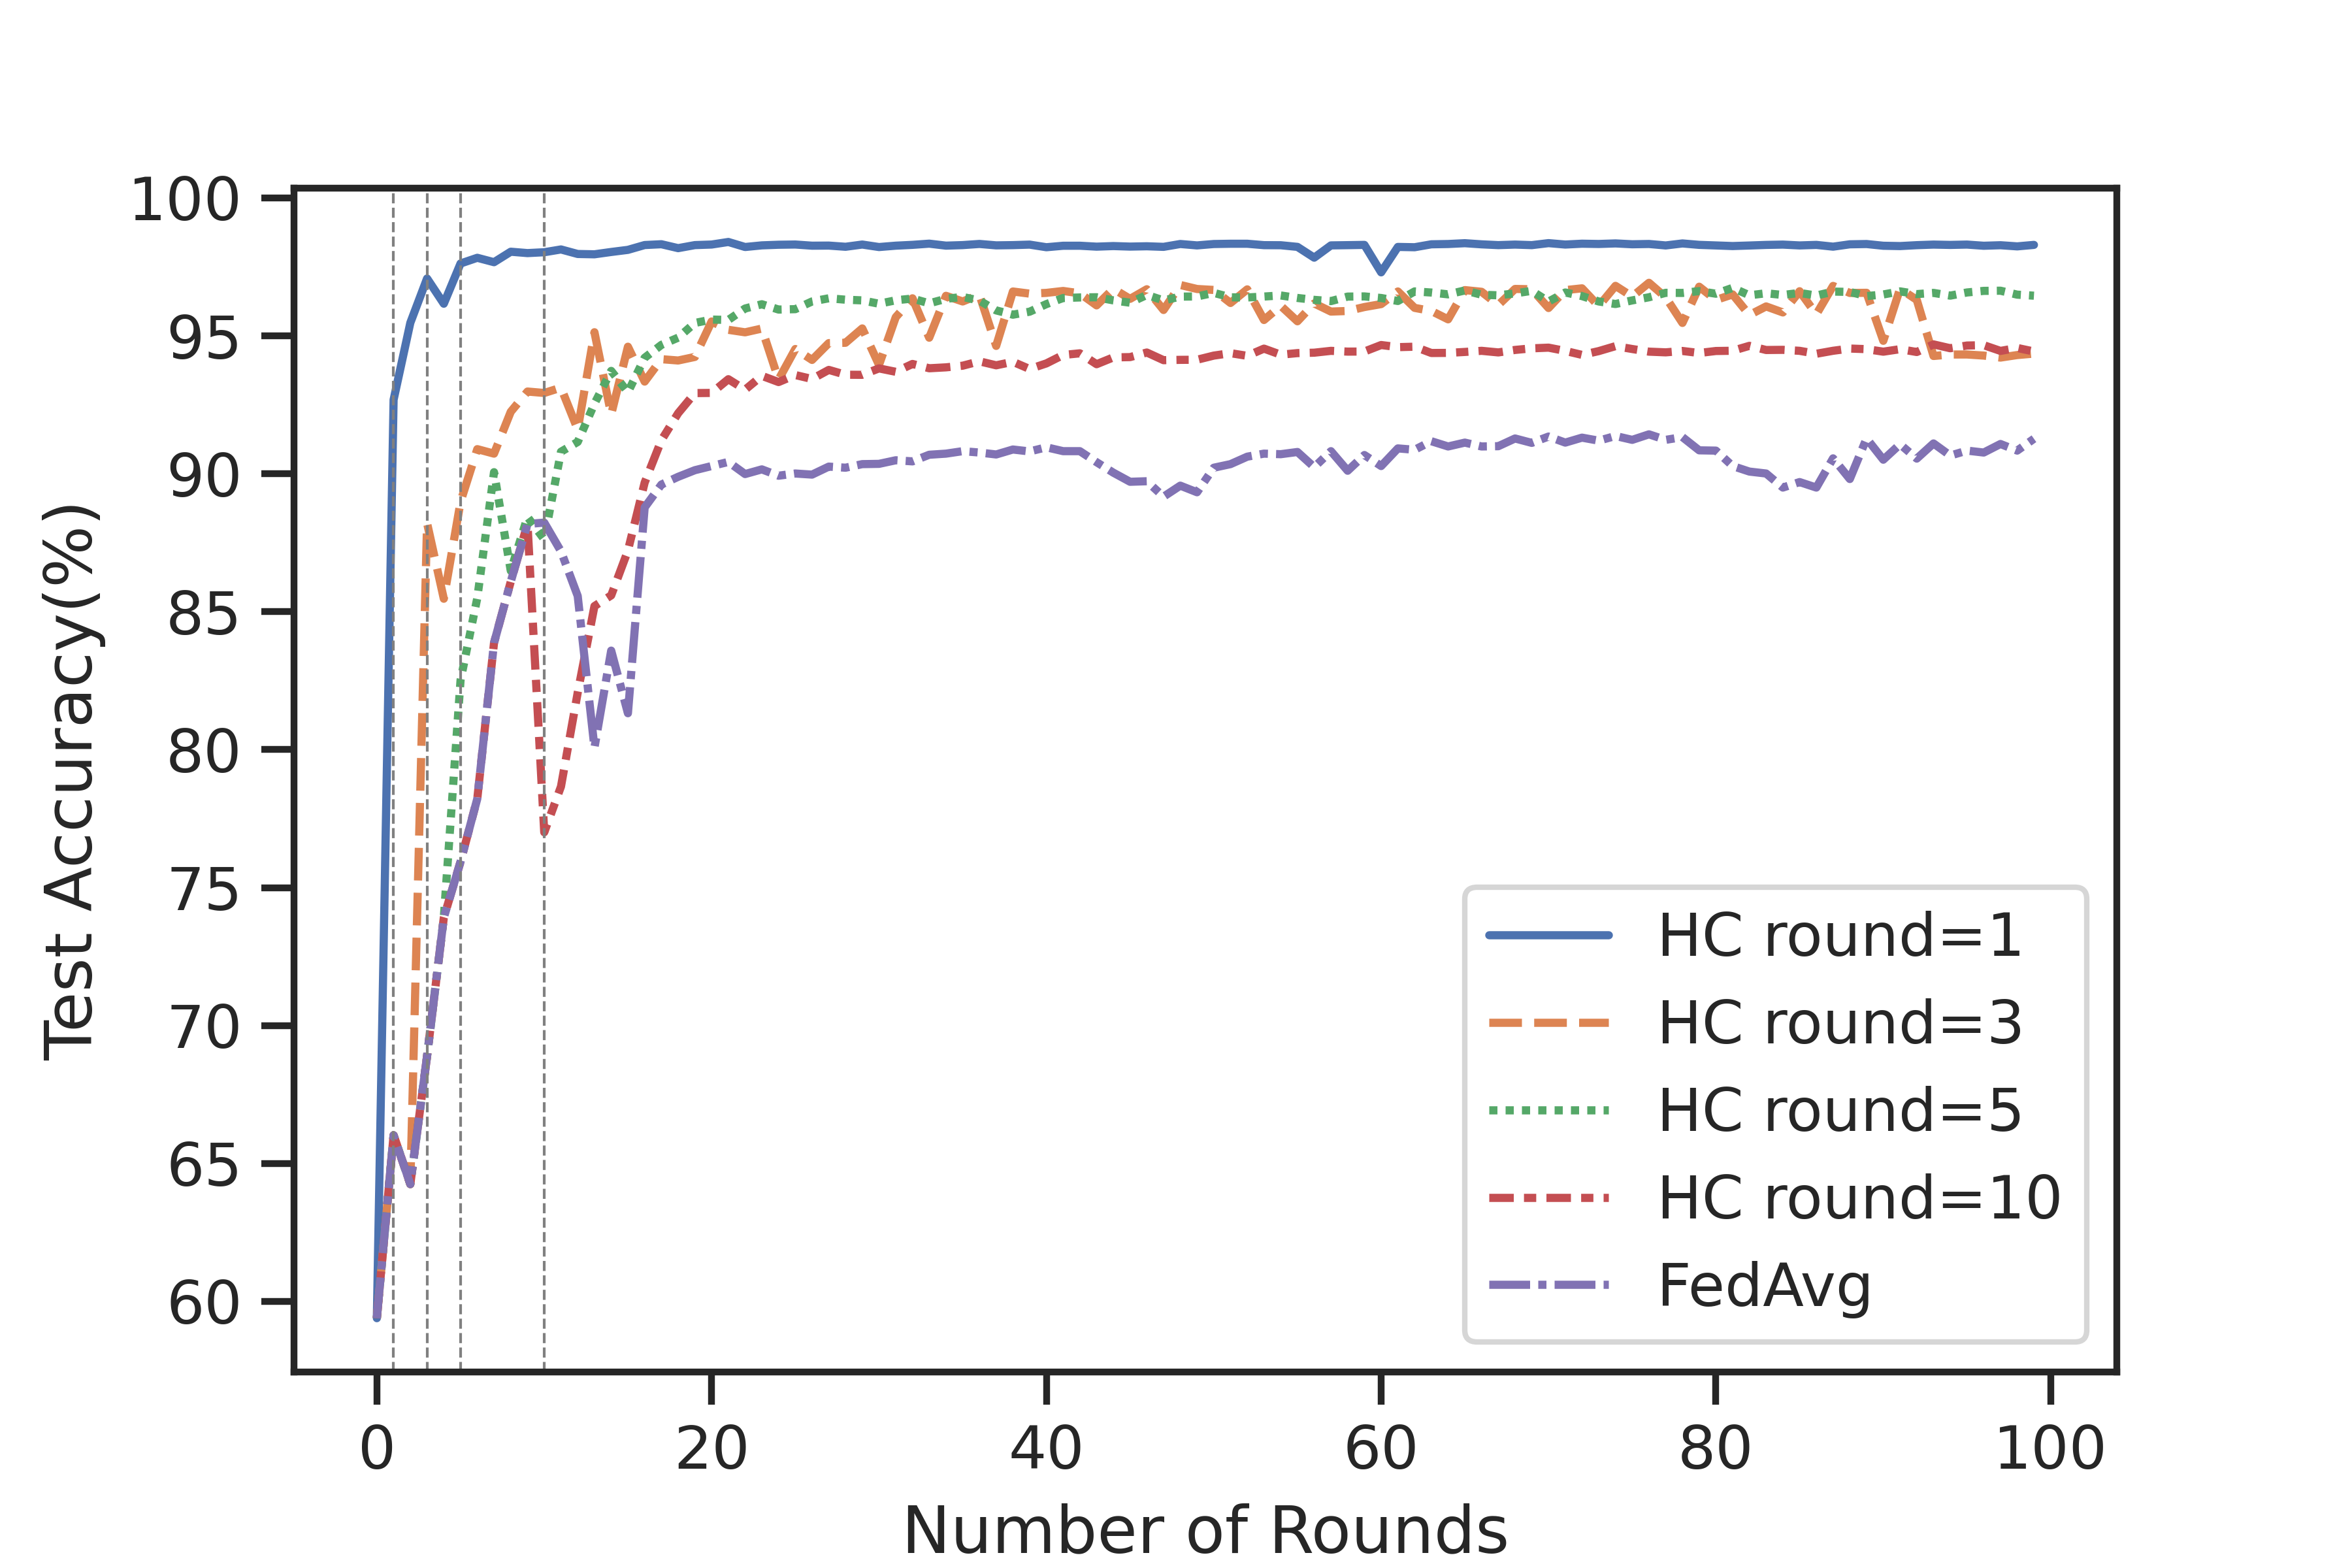
\includegraphics[width=\linewidth]{figs/mnist-noniid1}
%		\caption{Image 1}
%		\label{fig:image1}
%	\end{minipage}
%	\hspace{0.5cm}
%	\begin{minipage}[b]{0.4\linewidth}
%		\centering
%		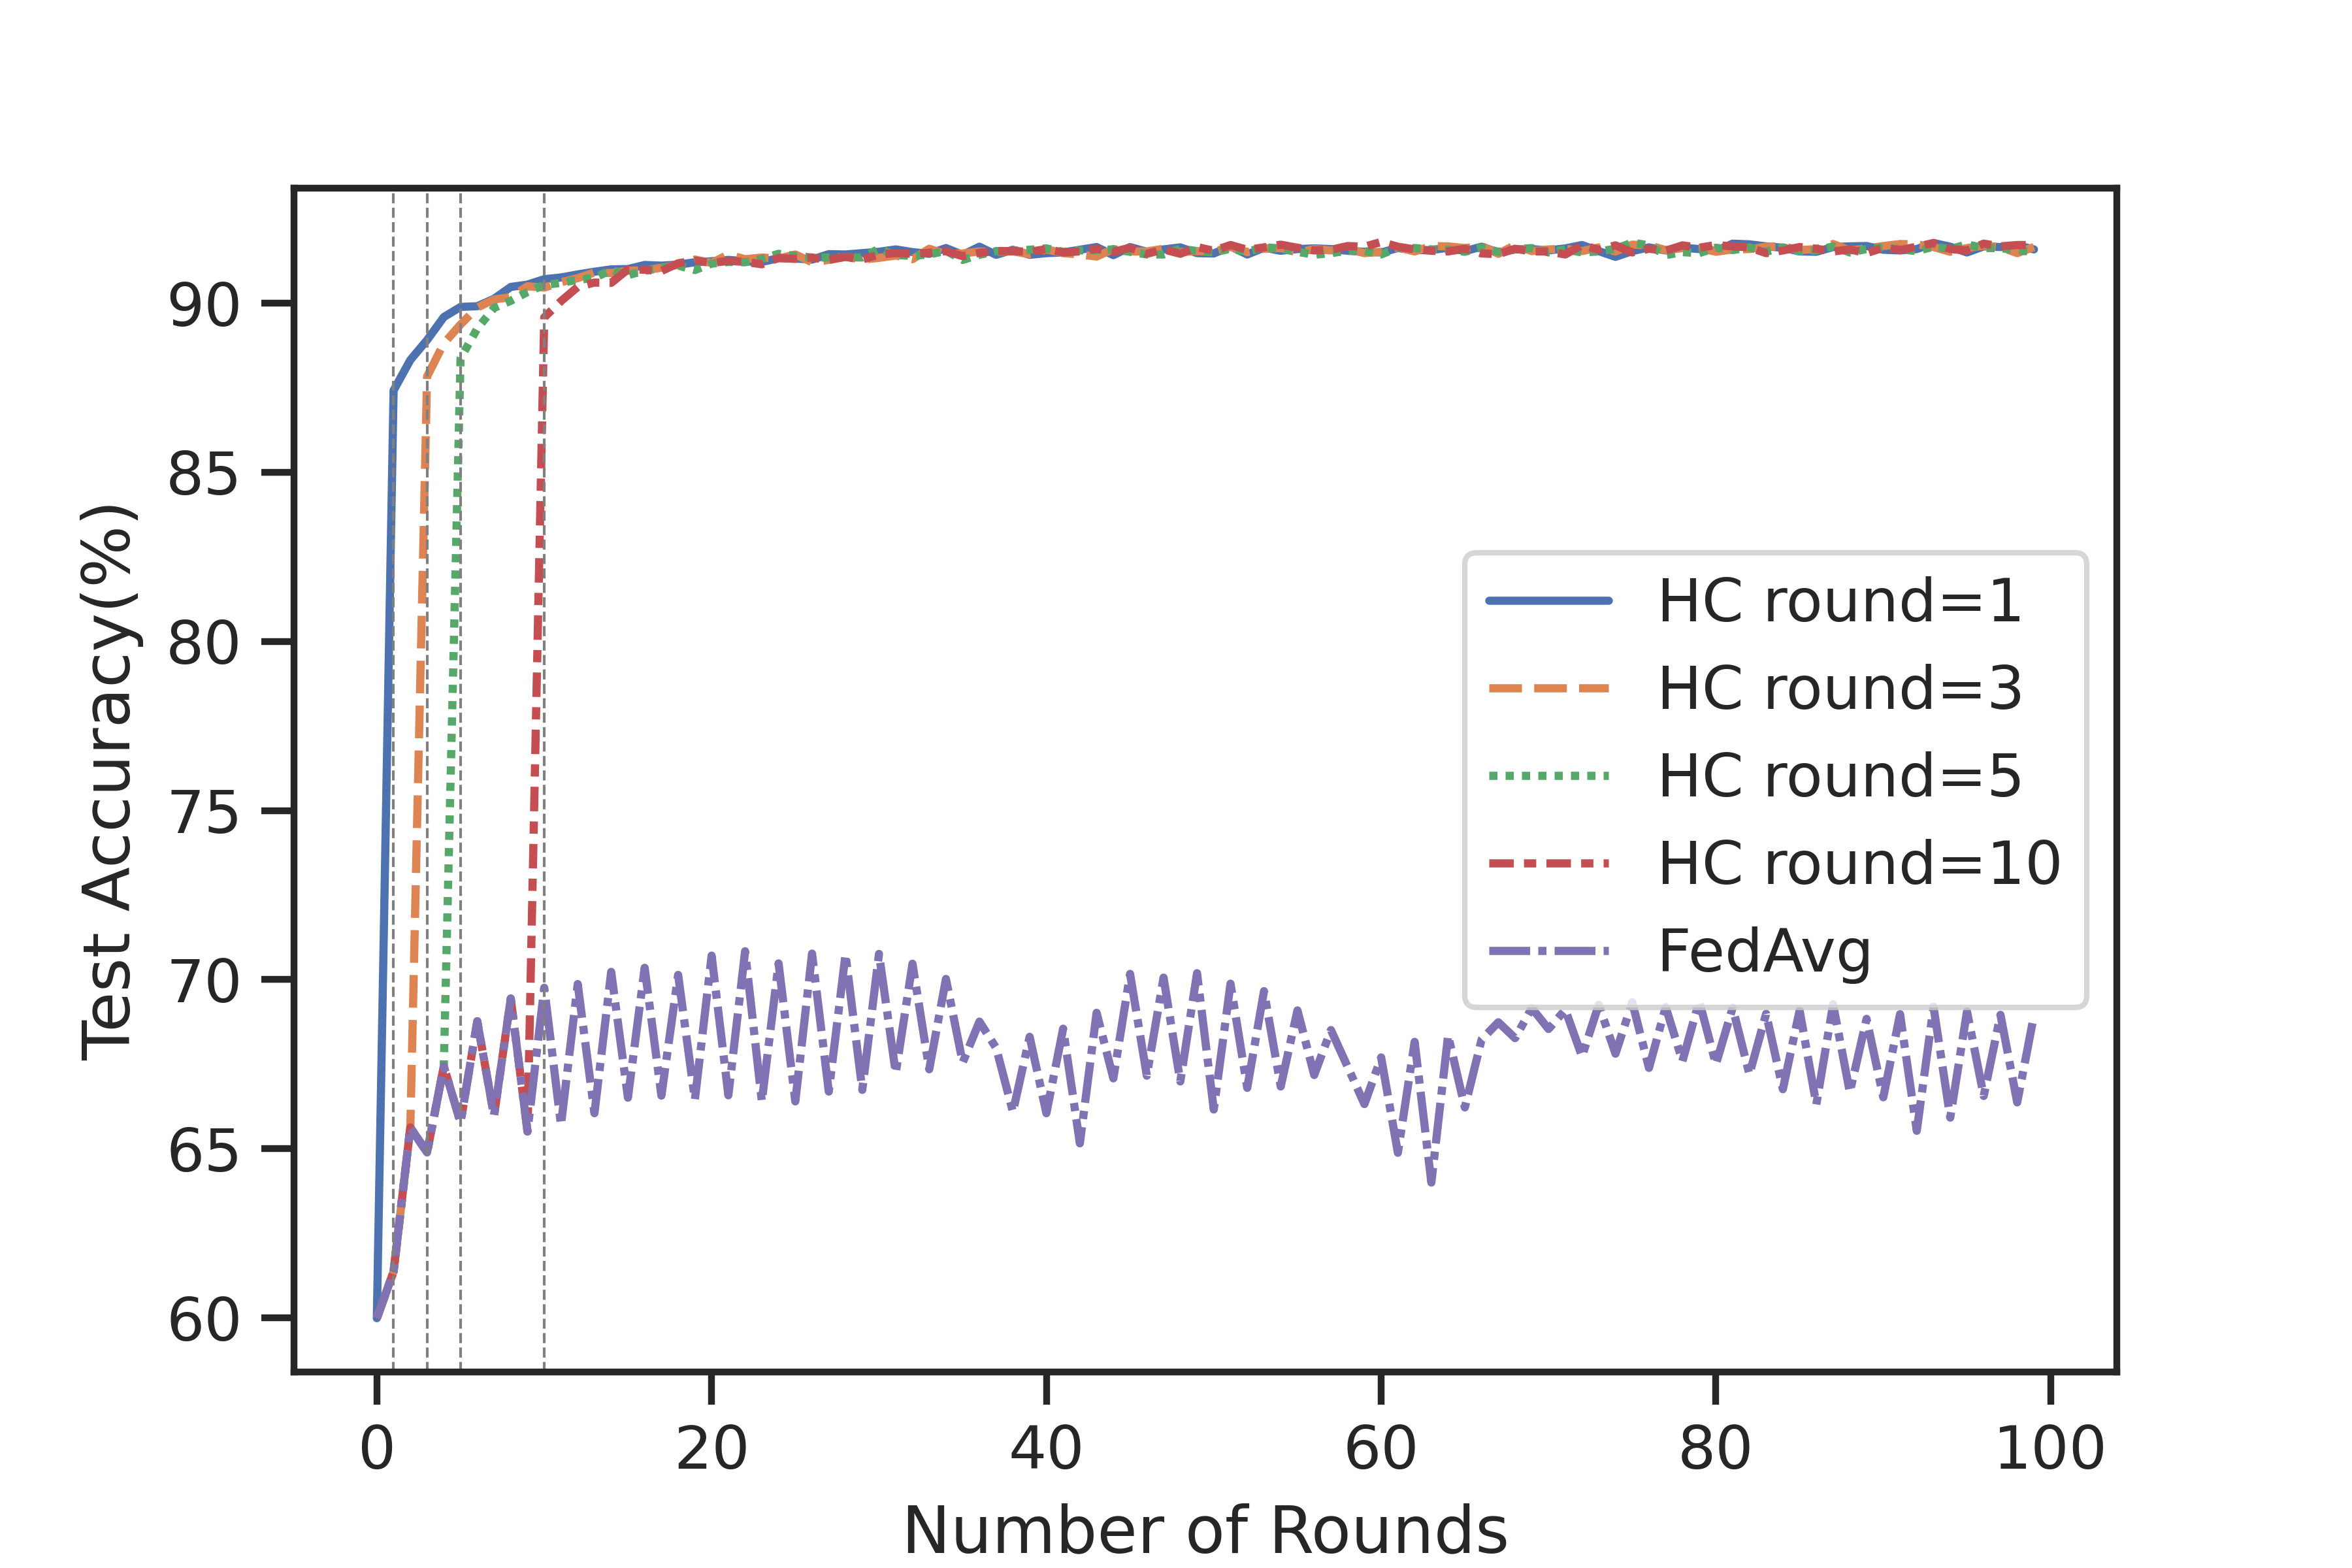
\includegraphics[width=\linewidth]{figs/mnist-noniid2}
%		\caption{Image 2}
%		\label{fig:image2}
%	\end{minipage}
%	\\
%		\begin{minipage}[b]{0.4\linewidth}
%		\centering
%		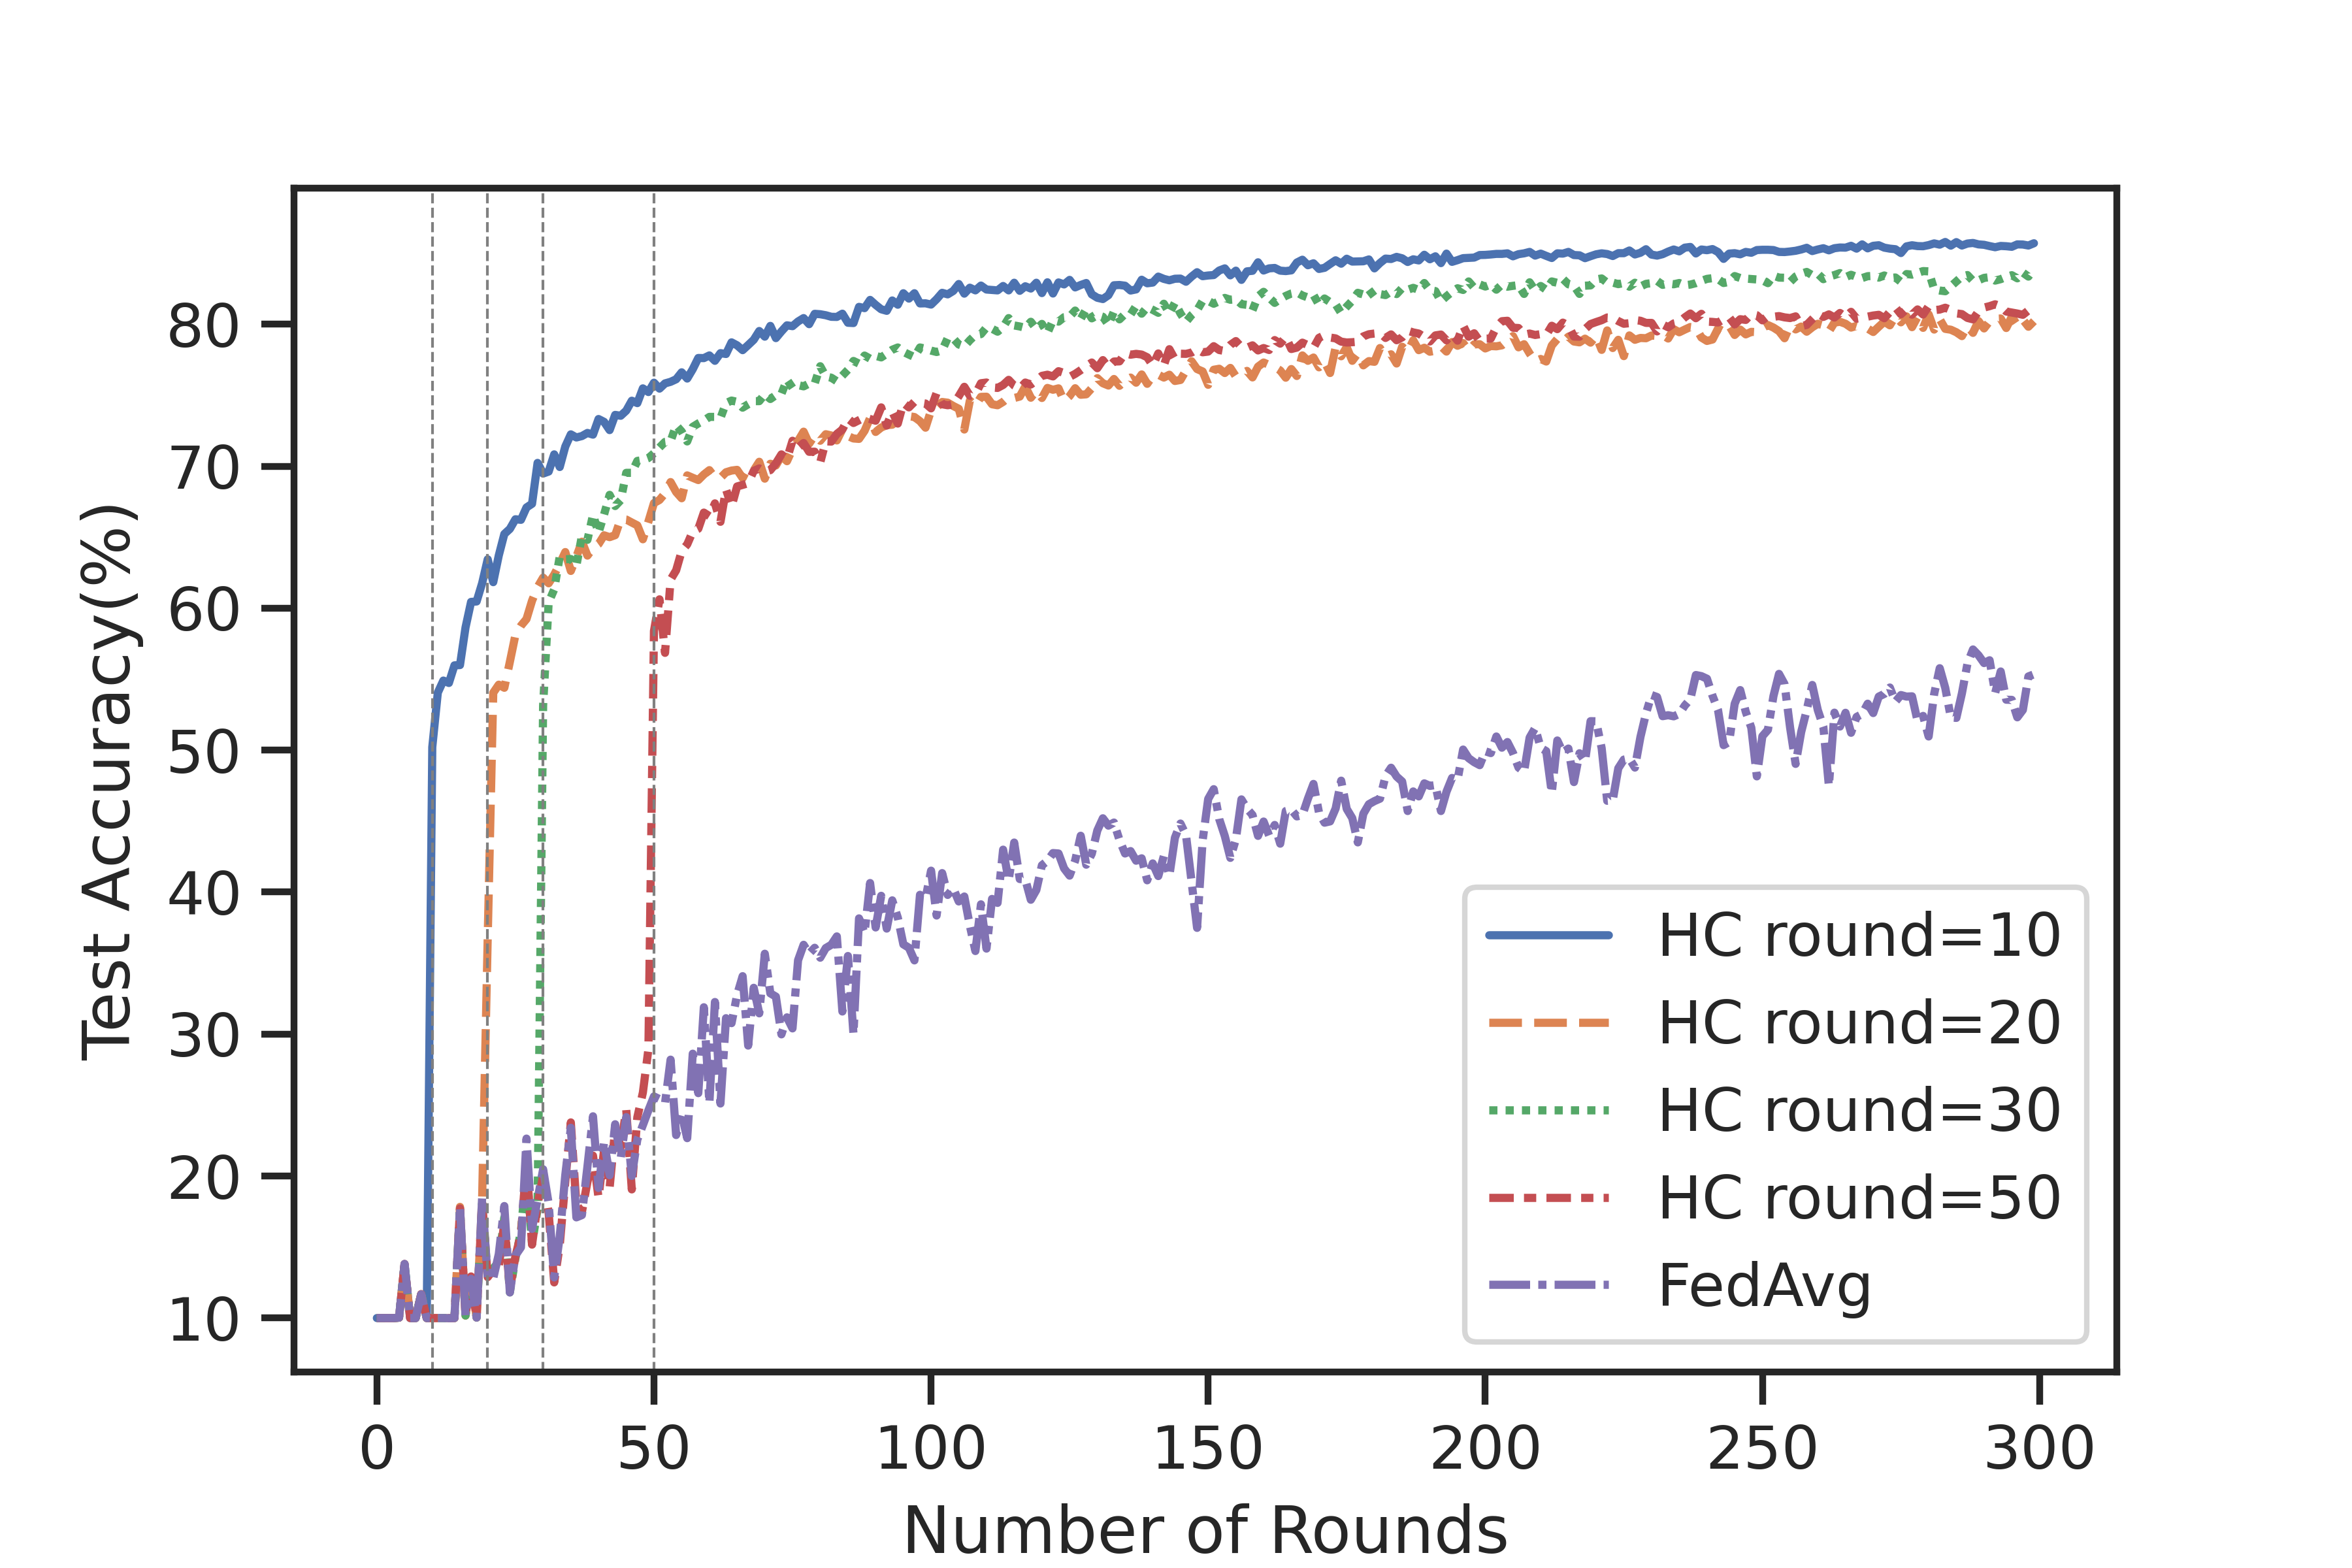
\includegraphics[width=\linewidth]{figs/cifar-noniid1}
%		\caption{Image 1}
%		\label{fig:image3}
%	\end{minipage}
%	\hspace{0.5cm}
%	\begin{minipage}[b]{0.4\linewidth}
%		\centering
%		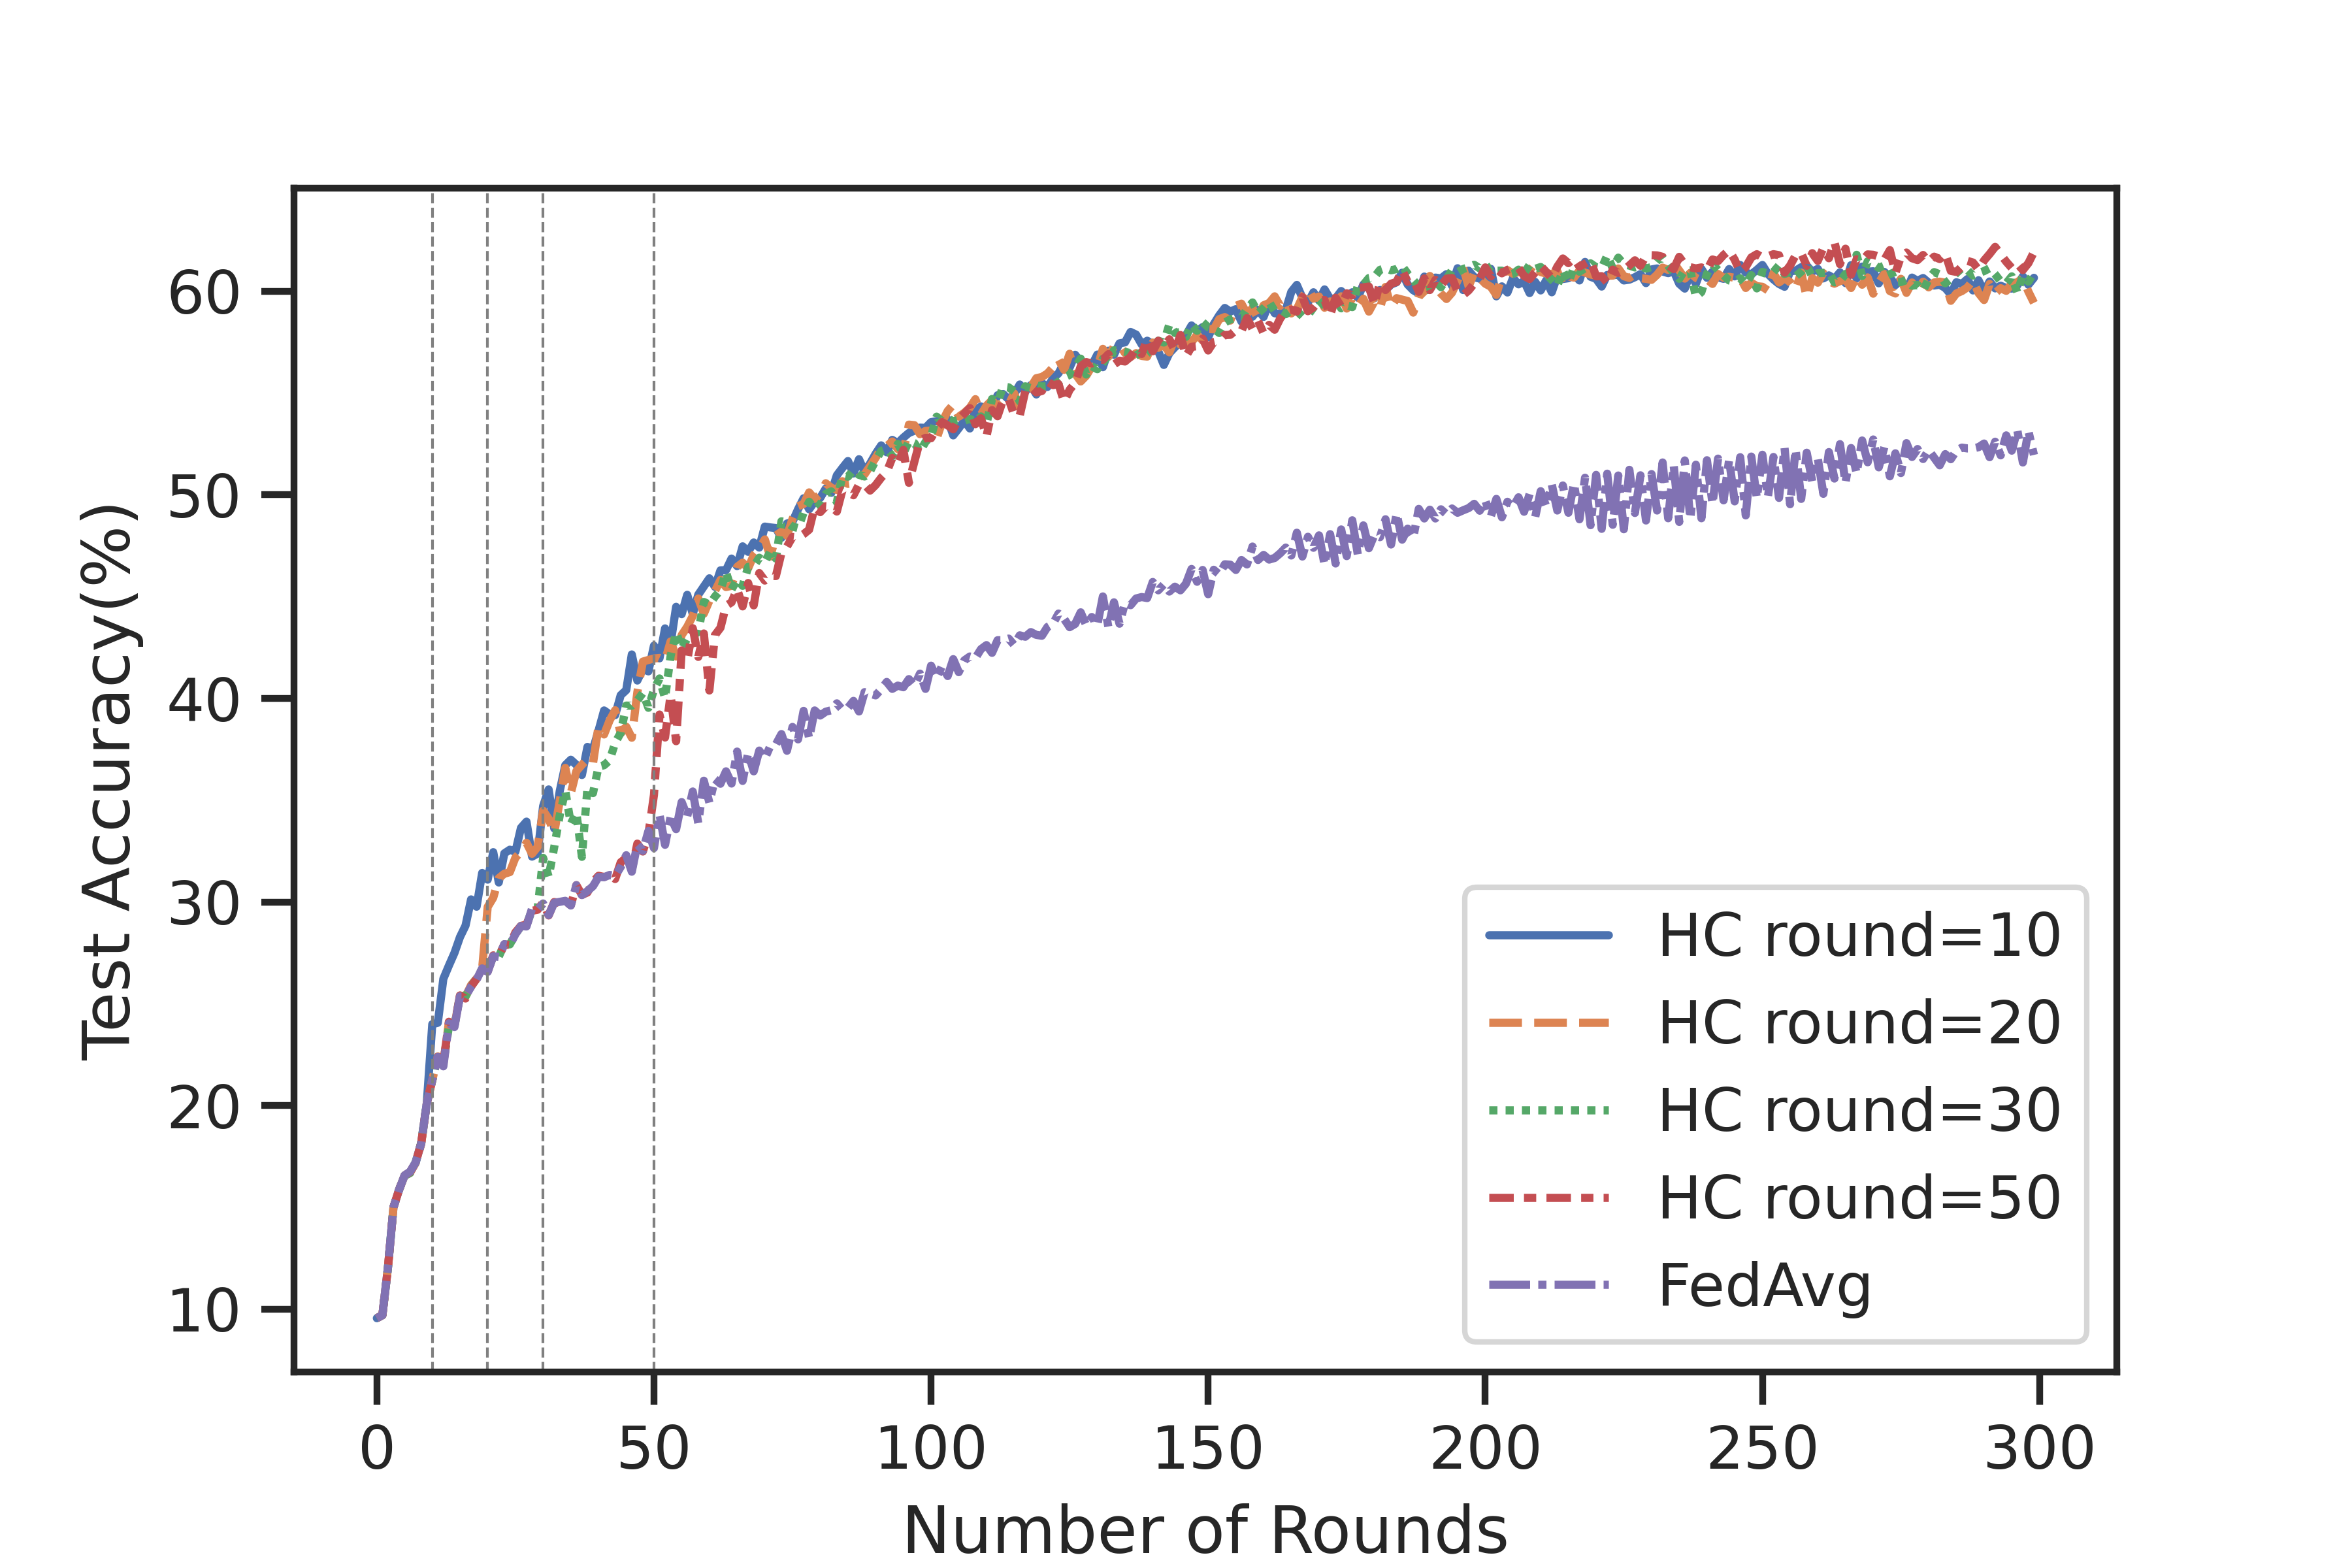
\includegraphics[width=\linewidth]{figs/cifar-noniid2}
%		\caption[i 4]{Image 2}
%		\label{fig:image4}
%	\end{minipage}
%%	\caption{Four images side by side.}
%	\label{fig:four_images}
%\end{figure}

\subsubsection{准确率测试}

许多因素都会影响全局模型的准确率,其中包括神经网络模型的容量,参与方数据的数量以及训练的轮次等,而本节关注的是PPFL+HC在异质分数数据场景下,对比经典FedAvg算法联合训练性能的提升。
因此首先变化聚合轮次,探究聚类操作的时机对全局模型准确率的影响。
注意因为针对CIFAR-10分类任务所用到的网络结构相对简单,所以整体上准确率偏低,本节实验分析的重点在于对比FedAvg准确率上的提升。

\textbf{不同异质分布数据类型的影响:}图\ref{fig-acc} 展示了不同数据集(MNIST和CIFAR-10)在不同异质分布数据场景下,不同的聚类轮次对于联合训练准确率的影响。表\ref{mnist-keyround}和表\ref{cifar-keyround}展示了聚类后轮次和最后轮次与FedAvg在准确率上的对比,其中括号内的数字表示与FedAvg相应轮次准确率的比值。
本文观察到,经过层次聚类之后,所有场景在最终的训练准确率上都有提升(1.04-1.57$\times$FedAvg),同时几乎所有的场景都在聚类后的第一个轮次就迎来了准确率的提升,
其中CIFAR-10数据集在分布偏差的异质分布数据中准确率增长最明显(5.0$\times$FedAvg)。
这表明PPFL+HC的安全层次聚类算法(SHC),可以很好的将拥有相似梯度的参与方分为一个簇,在同一个簇内联合生成全局模型,很好的避免了存在分歧的梯度的影响,因此提高了整体全局模型的性能。

{\wuhao
\begin{figure}[htb]
	\centering
	\subfloat[MNIST数据集在分布偏差的异质分布数据下,随训练轮次以及聚类轮次变化的的测试准确率]{
		%		\begin{minipage}[b]{0.27\textwidth}
			\centering
			\label{fig-acc:a}
			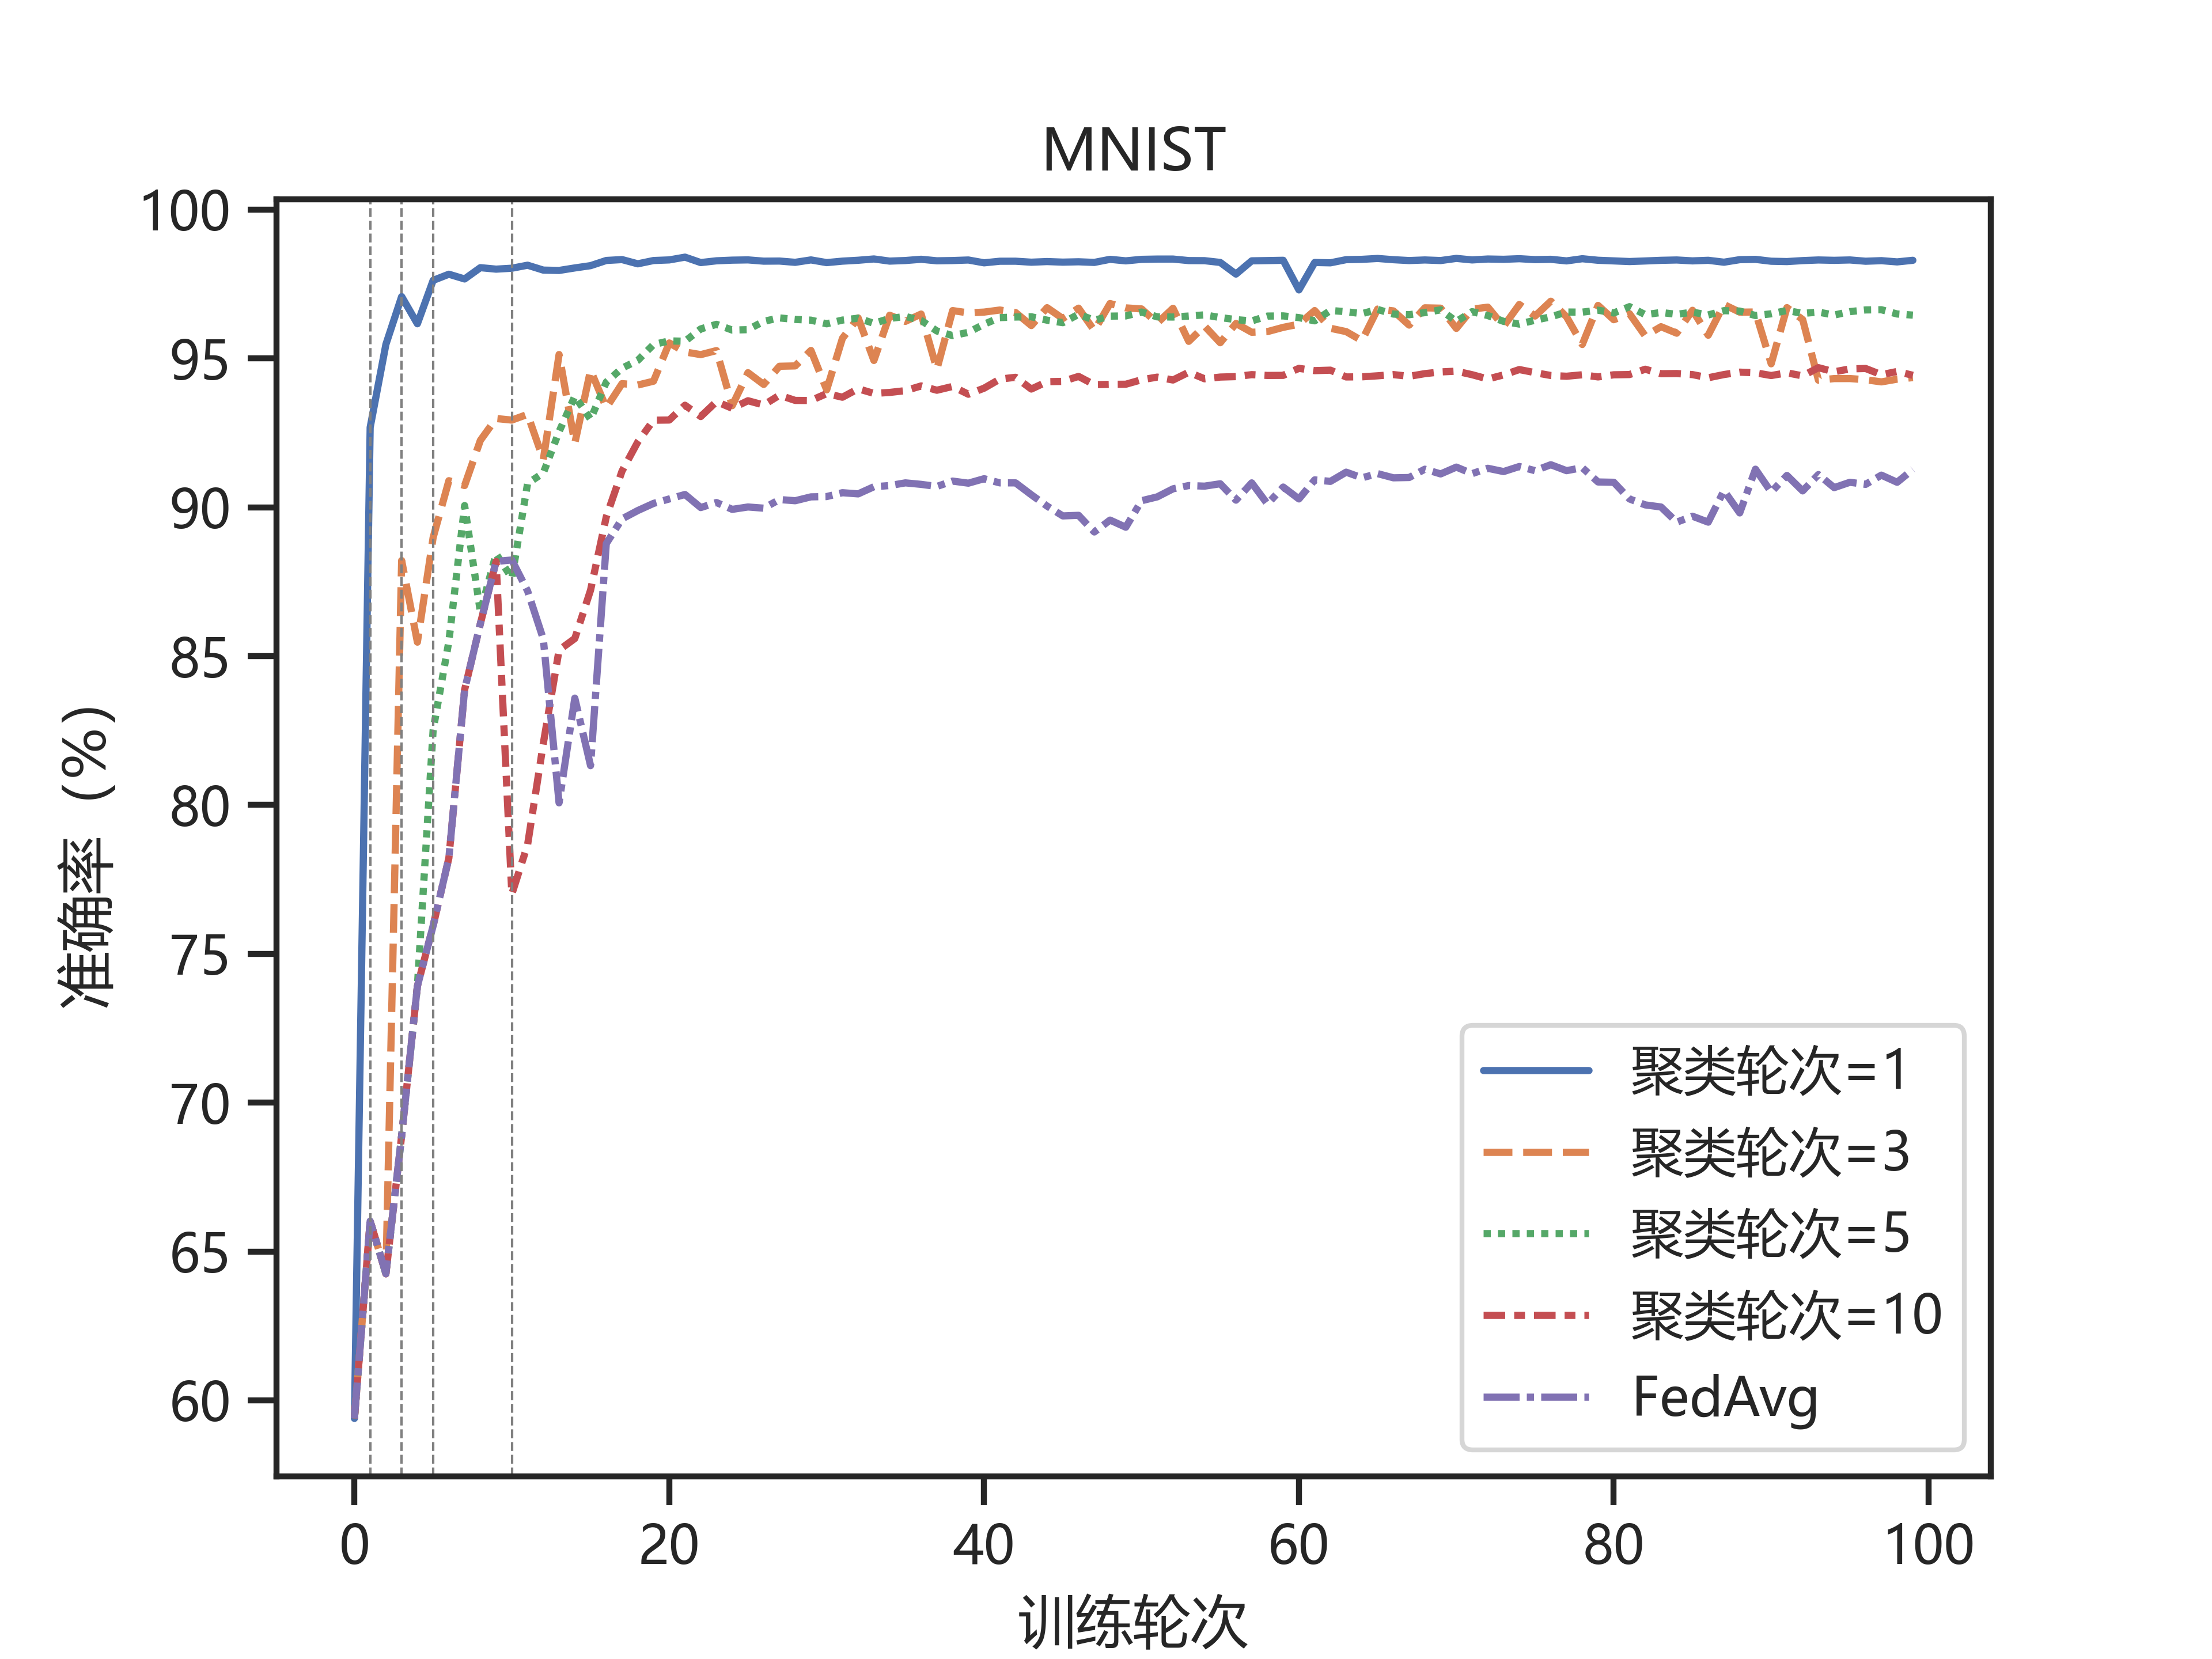
\includegraphics[width=0.45\columnwidth]{figs/mnist-noniid-win-1}
			%		\end{minipage}
	}
	\qquad
	\subfloat[MNIST数据集在标签交换的异质分布数据下,随训练轮次以及聚类轮次变化的的测试准确率]{
		%		\begin{minipage}[b]{0.27\textwidth}
			\centering
			\label{fig-acc:b}
			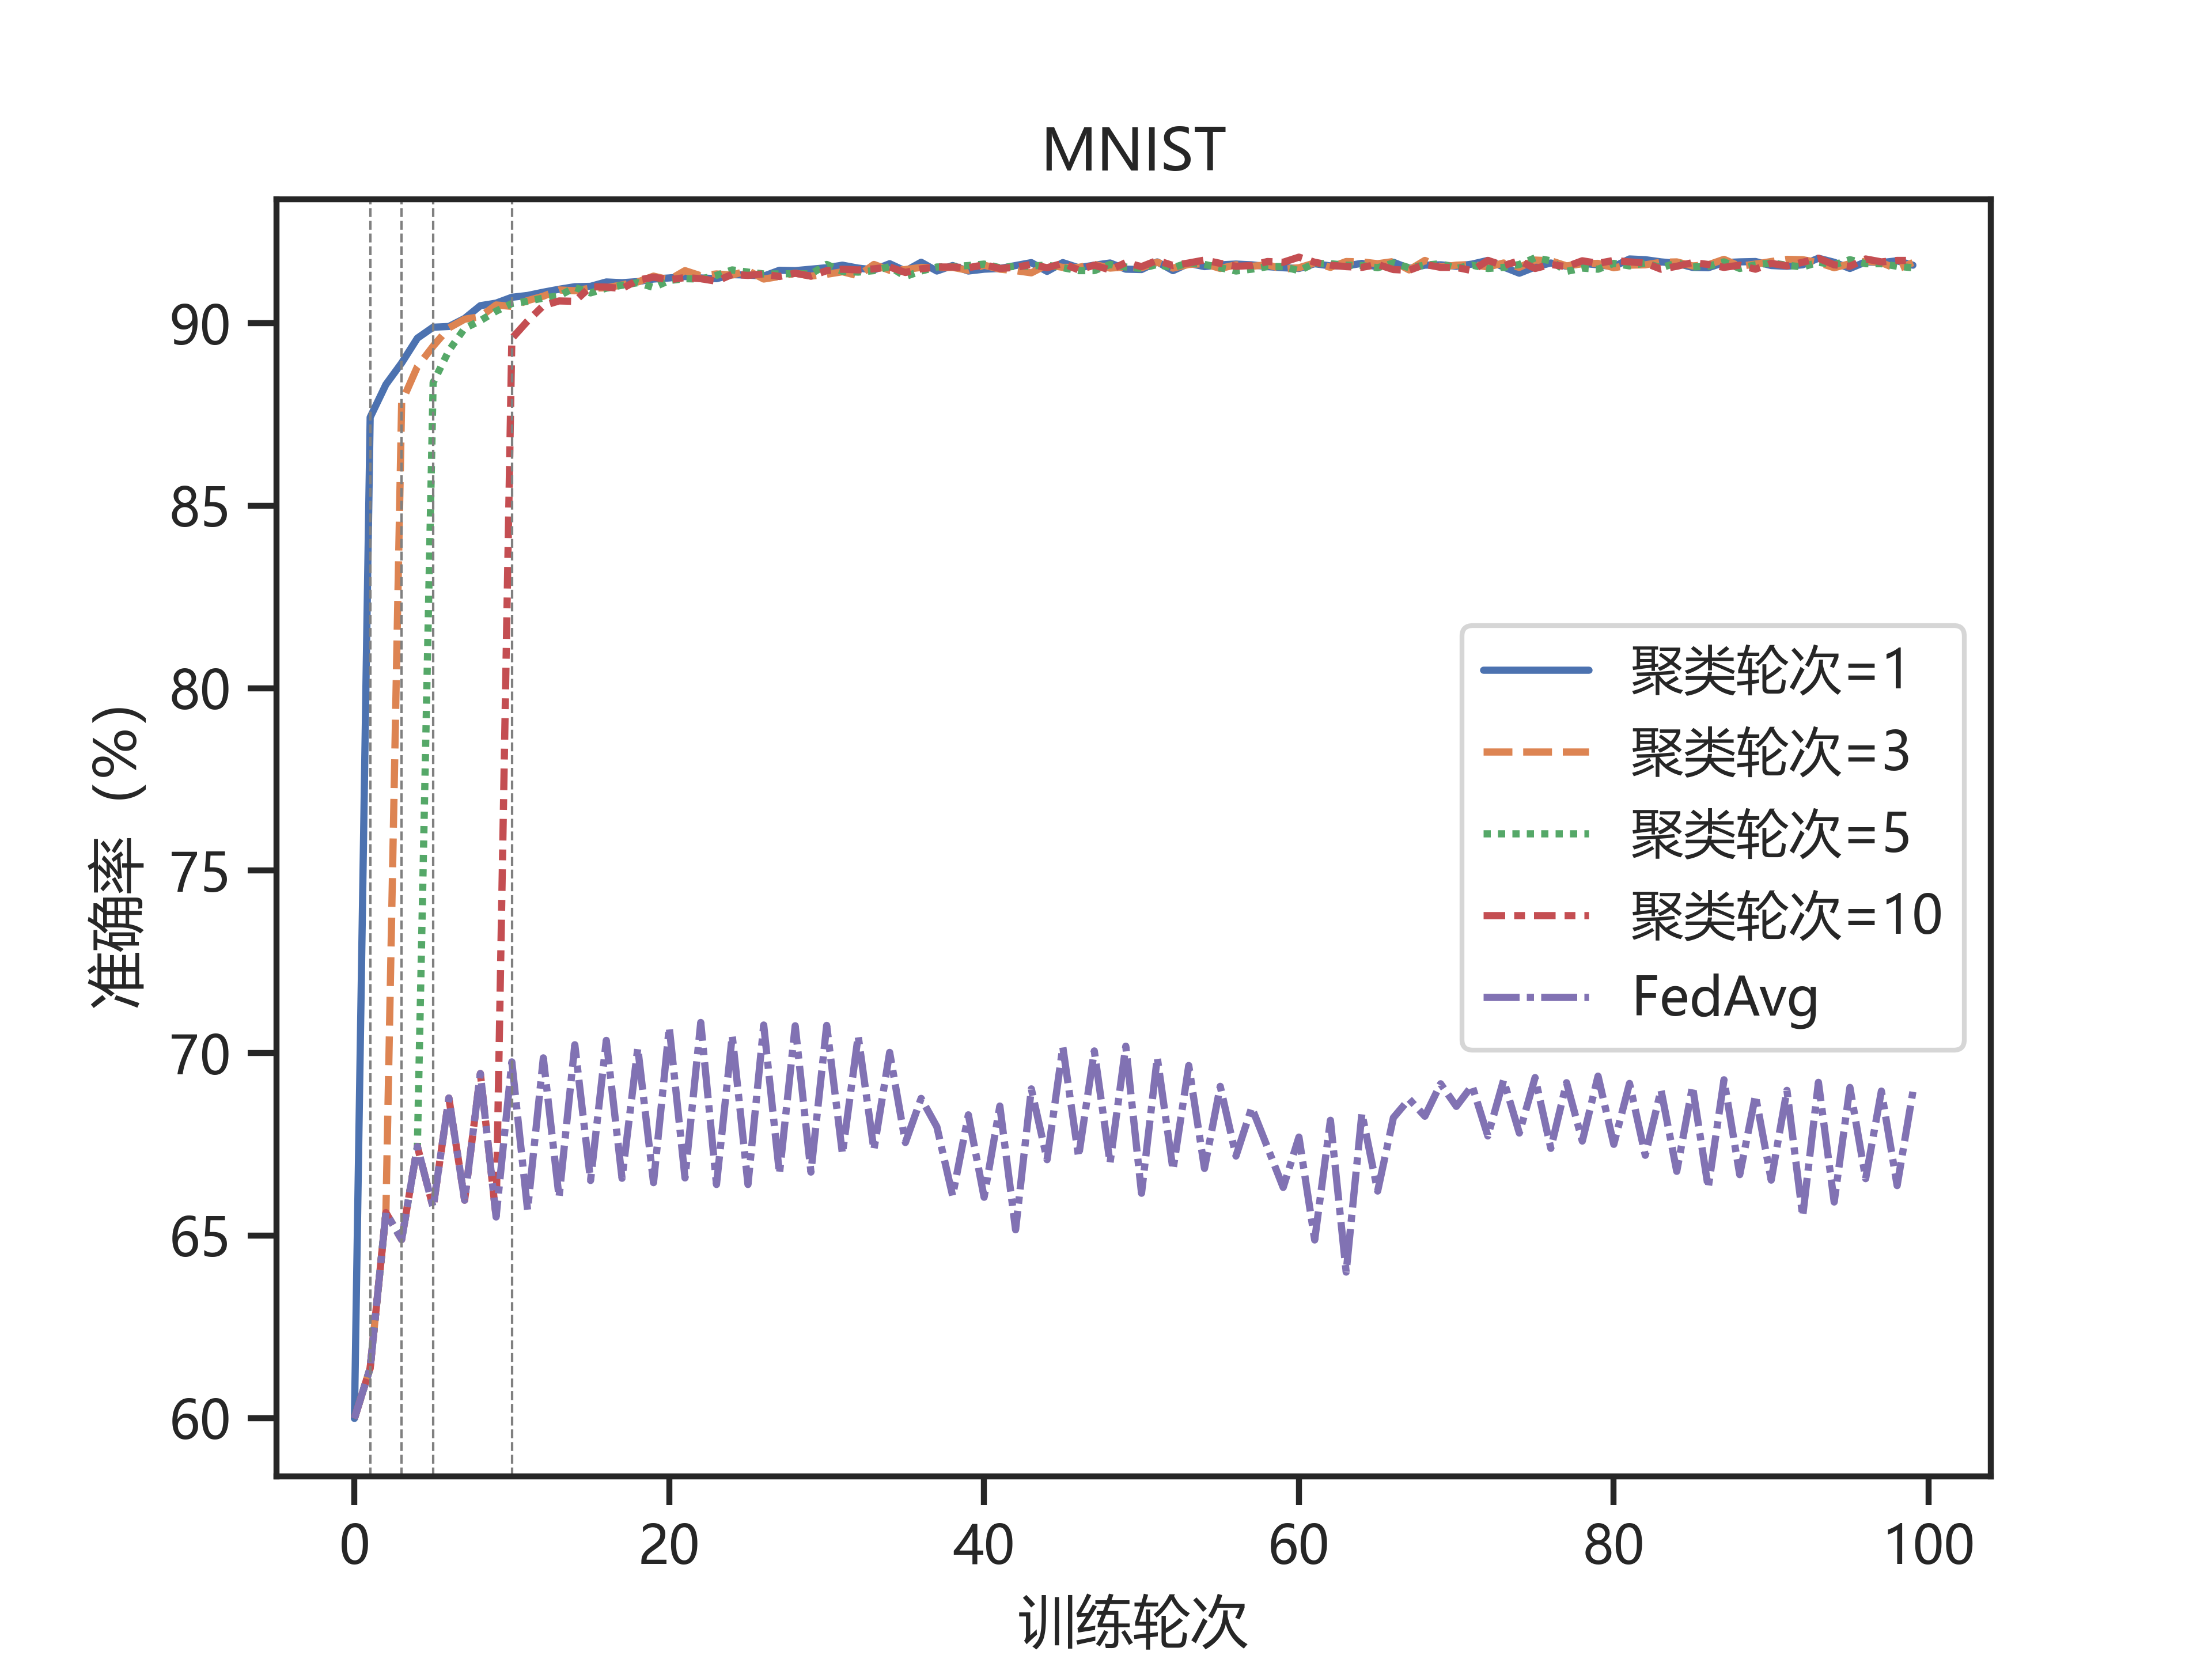
\includegraphics[width=0.45\columnwidth]{figs/mnist-noniid-win-2}
			%		\end{minipage}
	}
	\\
	\subfloat[CIFAR-10数据集在分布偏差的异质分布数据下,随训练轮次以及聚类轮次变化的的测试准确率]{
		%		\begin{minipage}[b]{0.27\textwidth}
			\centering
			\label{fig-acc:c}
			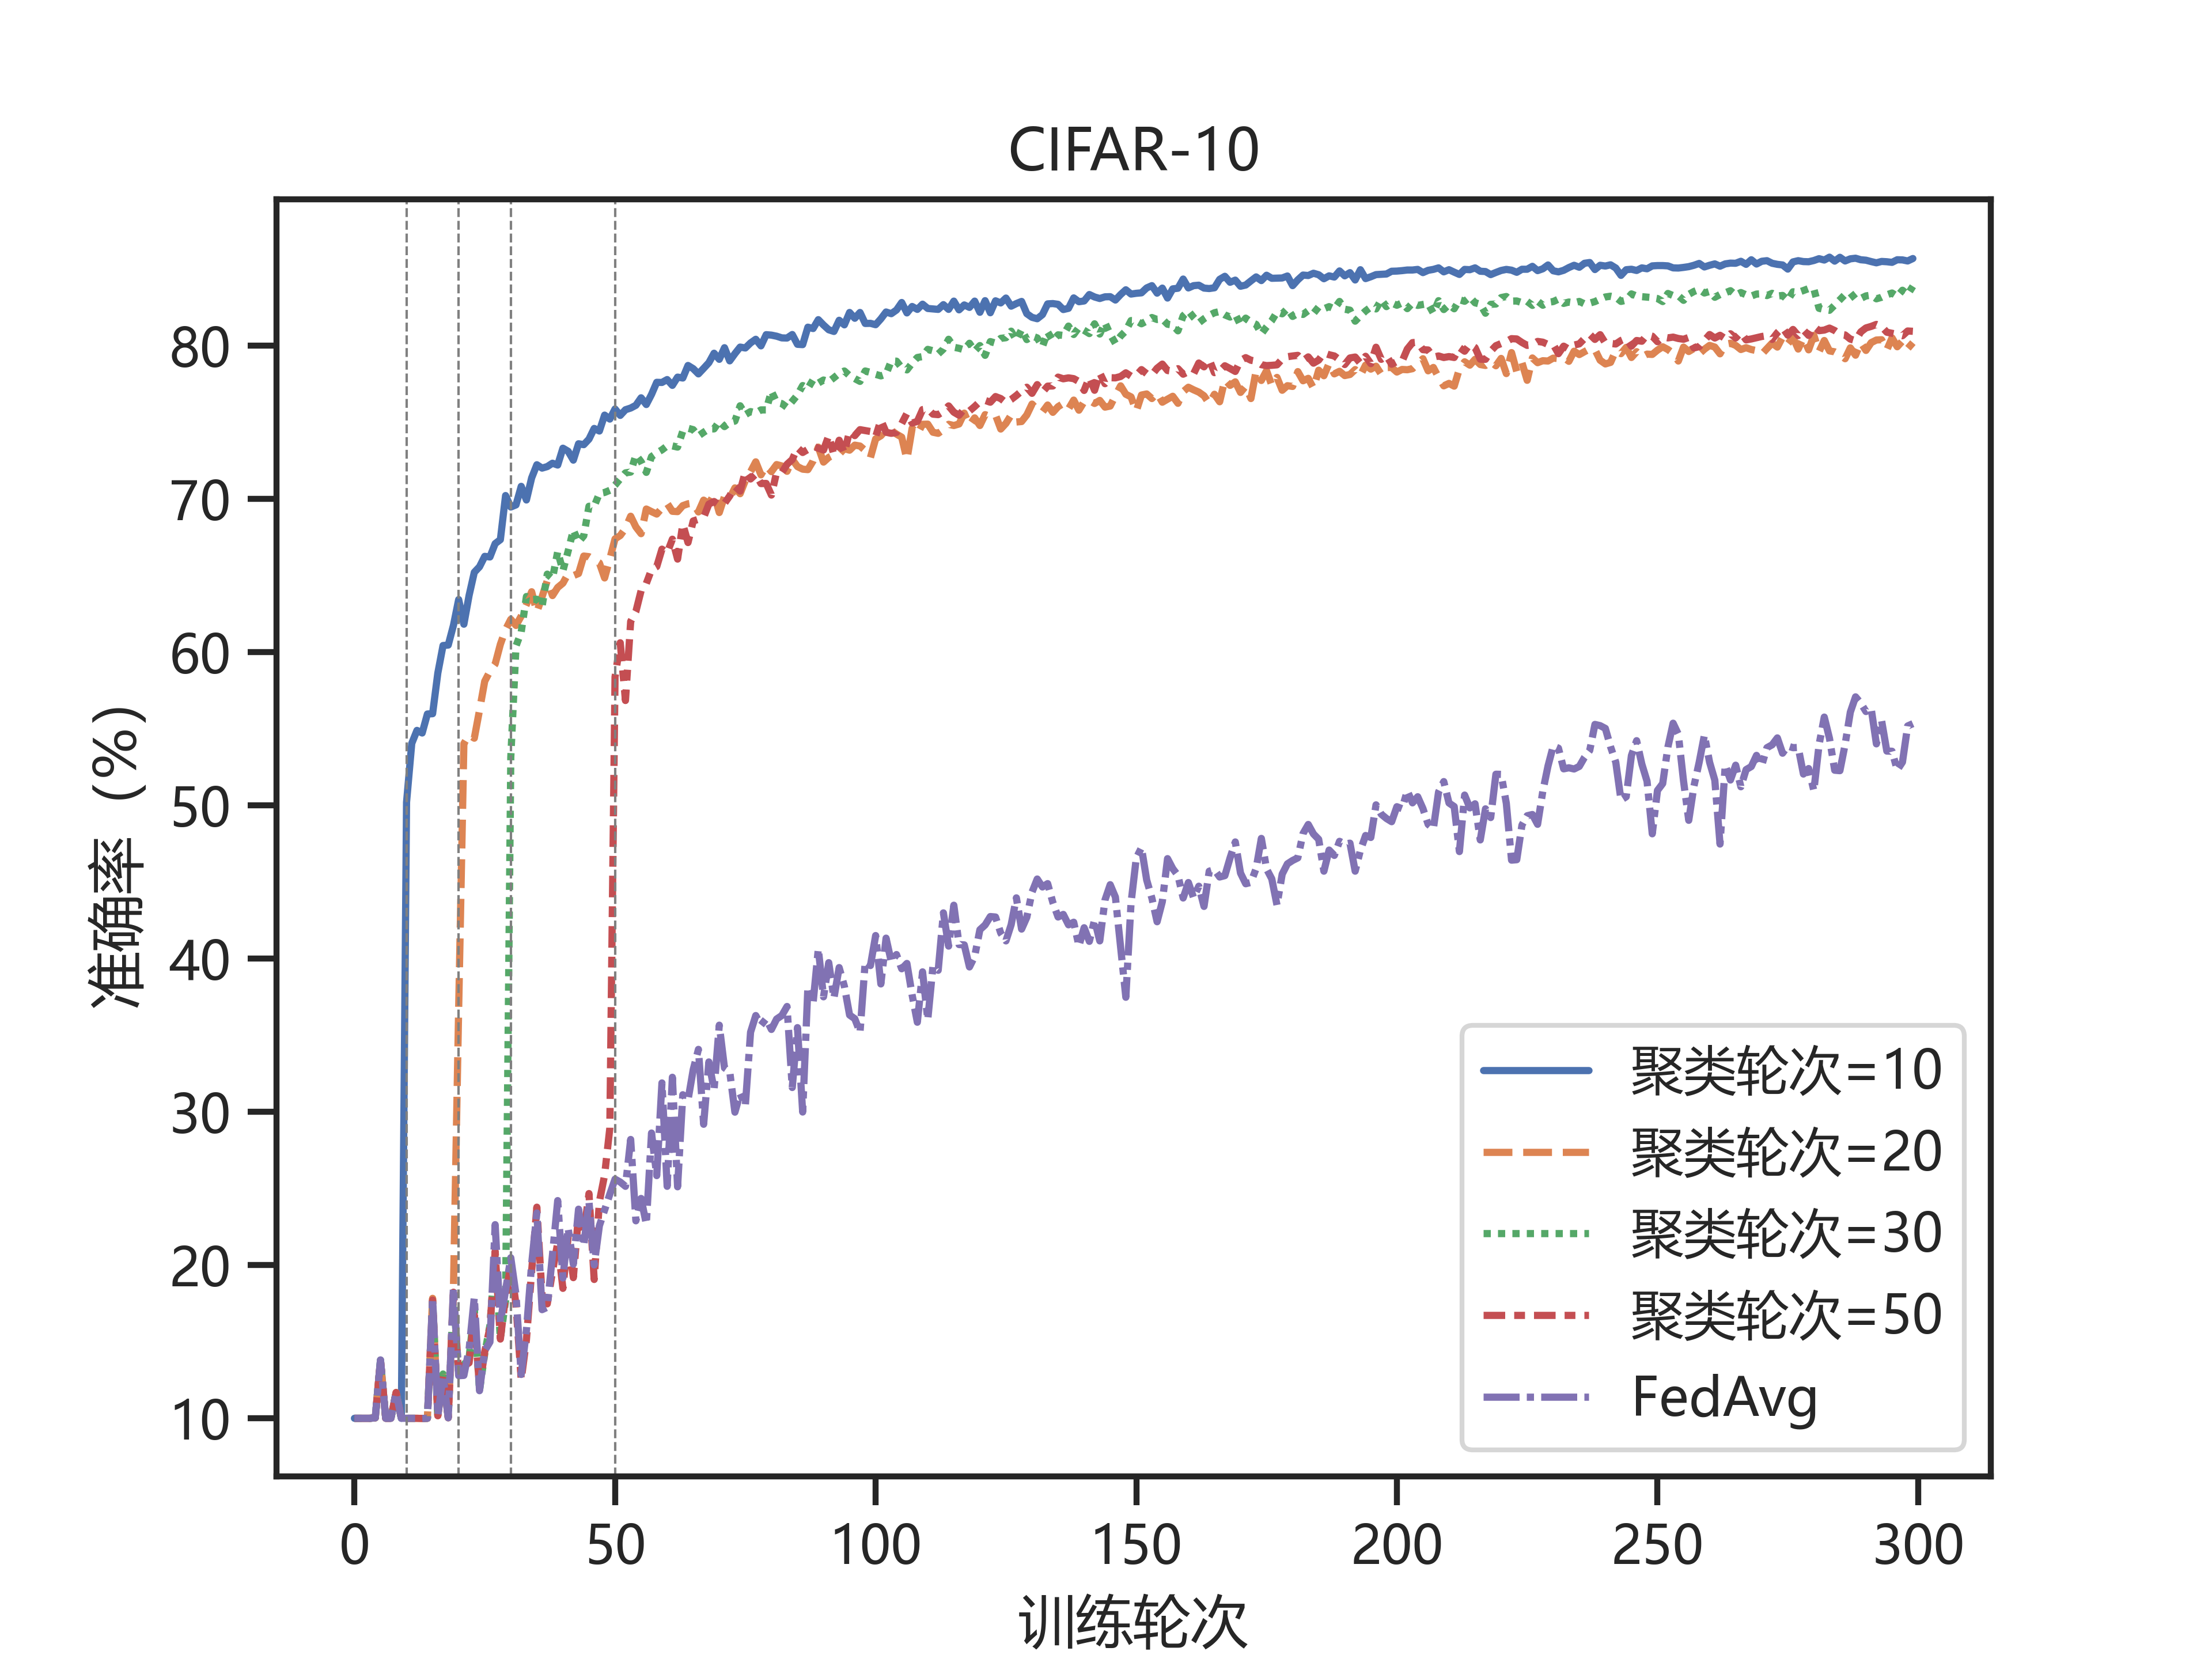
\includegraphics[width=0.45\linewidth]{figs/cifar-noniid-win-1.png}
			%		\end{minipage}
	}
	\qquad
	\subfloat[CIFAR-10数据集在标签交换的异质分布数据下,随训练轮次以及聚类轮次变化的的测试准确率]{
		%		\begin{minipage}[b]{0.27\textwidth}
			\centering
			\label{fig-acc:d}
			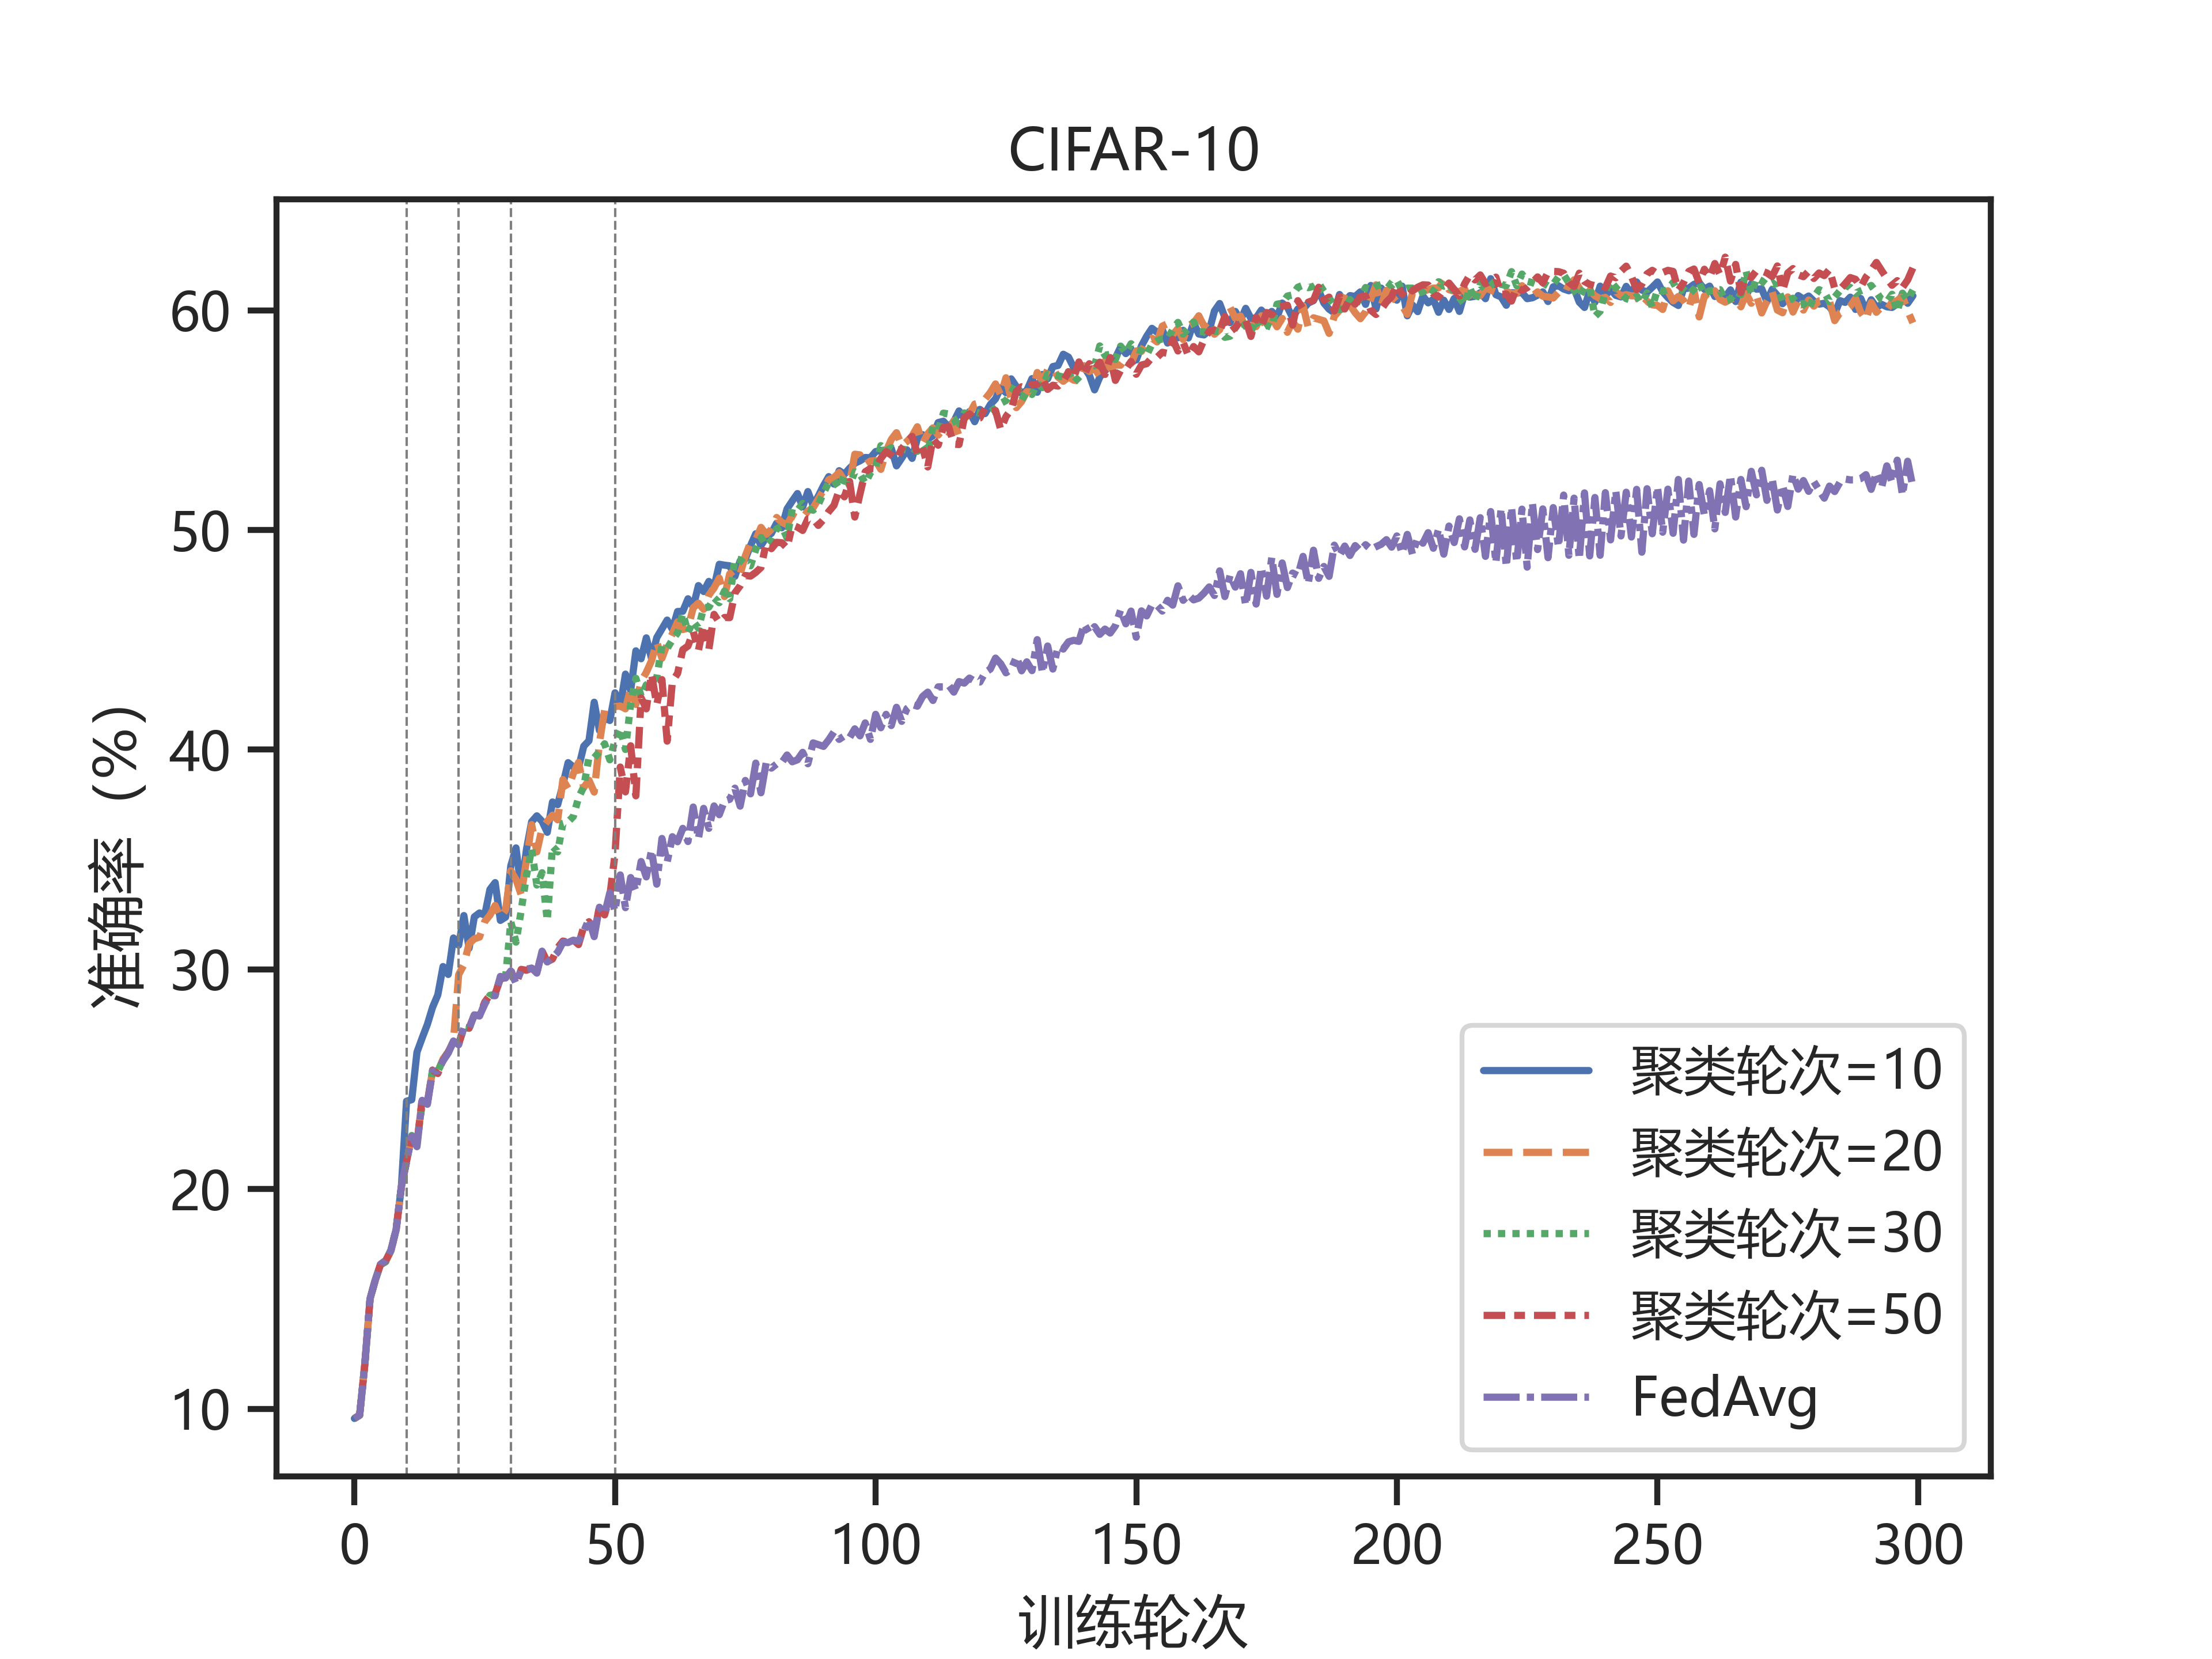
\includegraphics[width=0.45\columnwidth]{figs/cifar-noniid-win-2}
			%		\end{minipage}
	}
	\caption[PPFL+HC准确率评估]{不同异质分布数据、不同训练轮次以及聚类轮次对测试准确率的影响,在图\ref{fig-acc:a} 和\ref{fig-acc:b}中,使用MNIST数据集来评估;在图\ref{fig-acc:c}和\ref{fig-acc:d}中,使用CIFAR-10数据集来评估。}
	\label{fig-acc}
\end{figure}
}

\begin{table}[]
	\centering
	\caption{MNIST关键轮次准确率对比}
	\label{mnist-keyround}
%	\begin{minipage}[t]{0.6\linewidth}
	\scalebox{0.87}{
	\begin{tabular}{cll|cll}
		\toprule
		\multicolumn{3}{c|}{分布偏差的MNIST}                        & \multicolumn{3}{c}{标签交换的MNIST}                       \\ \midrule
		聚类轮次 & \multicolumn{1}{c}{聚类后准确率(\%)}  & 最后准确率(\%)    & 聚类轮次 & \multicolumn{1}{c}{聚类后准确率(\%)} & 最后准确率(\%)    \\
		1    & 92.68(1.4x)$^*$ & 98.28(1.08x) & 1    & 87.42(1.42x)                   & 91.63(1.36x) \\
		3    & 88.21(1.28x)                    & 94.79(1.04x) & 3    & 87.83(1.35x)                   & 91.65(1.36x) \\
		5    & 82.52(1.09x)                    & 96.54(1.06x) & 5    & 88.37(1.35x)                   & 91.61(1.36x) \\
		10   & 77.00(0.87x)                    & 94.54(1.04x) & 10   & 89.58(1.28x)                   & 91.67(1.36x) \\ \bottomrule
	\end{tabular}
	}
\begin{flushleft}
	\scalebox{0.87}{
	\footnotesize
	*:(1.4x) 表示准确率为1.4x FedAvg}
\end{flushleft}

%	\end{minipage}
\end{table}
%\footnote{表示此轮次的准确率为1.4$\times$FedAvg}
\begin{table}[]
	\centering
	\caption{CIFAR-10关键轮次准确率对比}
	\label{cifar-keyround}
	\scalebox{0.87}{
	\begin{tabular}{cll|cll}
		\toprule
		\multicolumn{3}{c|}{分布偏差的CIFAR-10}                    & \multicolumn{3}{c}{标签交换的CIFAR-10}                    \\ \midrule
		聚类轮次 & \multicolumn{1}{c}{聚类后准确率(\%)} & 最后准确率(\%)    & 聚类轮次 & \multicolumn{1}{c}{聚类后准确率(\%)} & 最后准确率(\%)    \\
		10   & 50.21(5x)                      & 85.54(1.57x) & 10   & 24.0(1.13x)                    & 60.32(1.15x) \\
		20   & 36.76(2.88x)                   & 80.12(1.47x) & 20   & 29.76(1.12x)                   & 60.09(1.15x) \\
		30   & 53.14(2.59x)                   & 83.37(1.53x) & 30   & 32.17(1.07x)                   & 60.67(1.16x) \\
		50   & 58.39(2.28x)                   & 81.01(1.49x) & 50   & 35.26(1.07x)                   & 61.56(1.17x) \\ \bottomrule
	\end{tabular}
	}
\end{table}

\subsubsection{聚类指标测试}\label{hc-test}
本节使用调整Rand系数(Adjusted Rand Index,ARI)\cite{hubert1985comparing}作为衡量聚类结果的指标。
ARI提供了正则化的输出,其输出范围在-1到1之间,ARI接近于1说明距离结果一致性较高,接近于0则说明聚类结果之间的关联近似于随机,而接近于-1表示聚类结果之间分歧较大。
以ARI作为聚类指标测试,可以判断出聚类结果之间的随机关联性,进而探明层次聚类是否捕捉到了梯度特征并进行正确的分类。
在标签交换的异质分布数据场景中,参与方持有的数据在划分时有明显的类别特征,分为四类,因此我们选择在这个场景对比不同因素对于梯度聚类结果的影响。
首先探究梯度的随机降维操作对聚类结果带来的影响,然后对比两种参数组合对于聚类结果的影响。

\textbf{梯度随机降维的影响:}表\ref{ari-sf-cmp}展示了两种数据集在不同的聚类轮次下,梯度的随机降维操作所使用到的梯度随机采样率对聚类结果的影响。
从表\ref{ari-sf-cmp}中可以看到,MNIST数据集产生的梯度在不同的聚类轮次和不同的采样率下,都能与真实分类结果完全一致,说明维度的降低不会对其聚类精度产生影响。
而对于CIFAR-10数据集,在采样率较大和聚类轮次较大的情况下,聚类精度较高。
而在采样率为0.1\%时(即维度为122),同时聚类轮次较小时,聚类精度相对较低,此时可以通过增大聚类轮次来获取较高的聚类精度。
综上,本文提出的梯度随机降维方法,在控制好采样率和聚类轮次的前提下,基本不会对聚类精度产生负面影响。

\begin{table}[]
	\centering
	\caption{不同梯度随机采样率ARI对比}
	\label{ari-sf-cmp}
	\scalebox{0.87}{
	\begin{tabular}{lllll|lllll}
		\toprule
		\multicolumn{5}{c|}{MNIST ARI}                                             & \multicolumn{5}{c}{CIFAR-10 ARI}                                          \\ \midrule
		\multicolumn{1}{c|}{\multirow{2}{*}{聚类轮次}} & \multicolumn{4}{l|}{梯度的随机采样率} & \multicolumn{1}{l|}{\multirow{2}{*}{聚类轮次}} & \multicolumn{4}{l}{梯度的随机采样率} \\ \cline{2-5} \cline{7-10} 
		\multicolumn{1}{c|}{}                      & 100\%  & 10\%  & 1\%  & 0.1\% & \multicolumn{1}{l|}{}                      & 100\%  & 10\% & 1\%  & 0.1\% \\ \hline
		\multicolumn{1}{c|}{1}                     & 1.0    & 1.0   & 1.0  & 1.0   & \multicolumn{1}{c|}{10}                    & 1.0    & 1.0  & 0.59 & 0.47  \\
		\multicolumn{1}{c|}{3}                     & 1.0    & 1.0   & 1.0  & 1.0   & \multicolumn{1}{c|}{20}                    & 1.0    & 1.0  & 0.92 & 0.71  \\
		\multicolumn{1}{c|}{5}                     & 1.0    & 1.0   & 1.0  & 1.0   & \multicolumn{1}{c|}{30}                    & 1.0    & 1.0  & 0.97 & 0.97  \\
		\multicolumn{1}{c|}{10}                    & 1.0    & 1.0   & 1.0  & 1.0   & \multicolumn{1}{c|}{50}                    & 1.0    & 1.0  & 1.0  & 0.97 \\ \bottomrule
	\end{tabular}
	}
\end{table}

\textbf{参数组合的影响:}本文提出的安全欧式距离计算算法和安全曼哈顿距离计算算法,可以作为层次聚类的安全距离度量方式,它们再搭配不同的簇间距离度量方式,就能完成对梯度的安全层次聚类。
本节的欧式距离搭配的簇间距离度量策略是沃德法(Ward Linkage),而曼哈顿距离搭配的是完全连接法(Complete Linkage)。
图\ref{hc-res-cmp}展示了在不同的梯度随机采样率下,这两种参数组合对于梯度聚类结果的影响(以不同聚类轮次的平均ARI来衡量)。
从图\ref{hc-res-cmp}中可以看到,MNIST数据集在两种参数组合下的表现都很优异,与真实分类结果完美匹配。
而对于CIFAR-10数据集,两种参数组合的平均ARI差距不大,且都随着采样率的升高而逐渐接近完美匹配。
综上,两种参数组合在对于梯度的聚类表现上差异不大,且都能在采样率不过低的前提下,完成高精度的聚类。

%聚类准确率ARI
{\wuhao
\begin{figure}[htb]
	\centering
	\subfloat[MNIST数据集平均ARI对比]{
		\begin{minipage}[b]{0.45\textwidth}
			\centering
			\label{hc-res-cmp:a}
			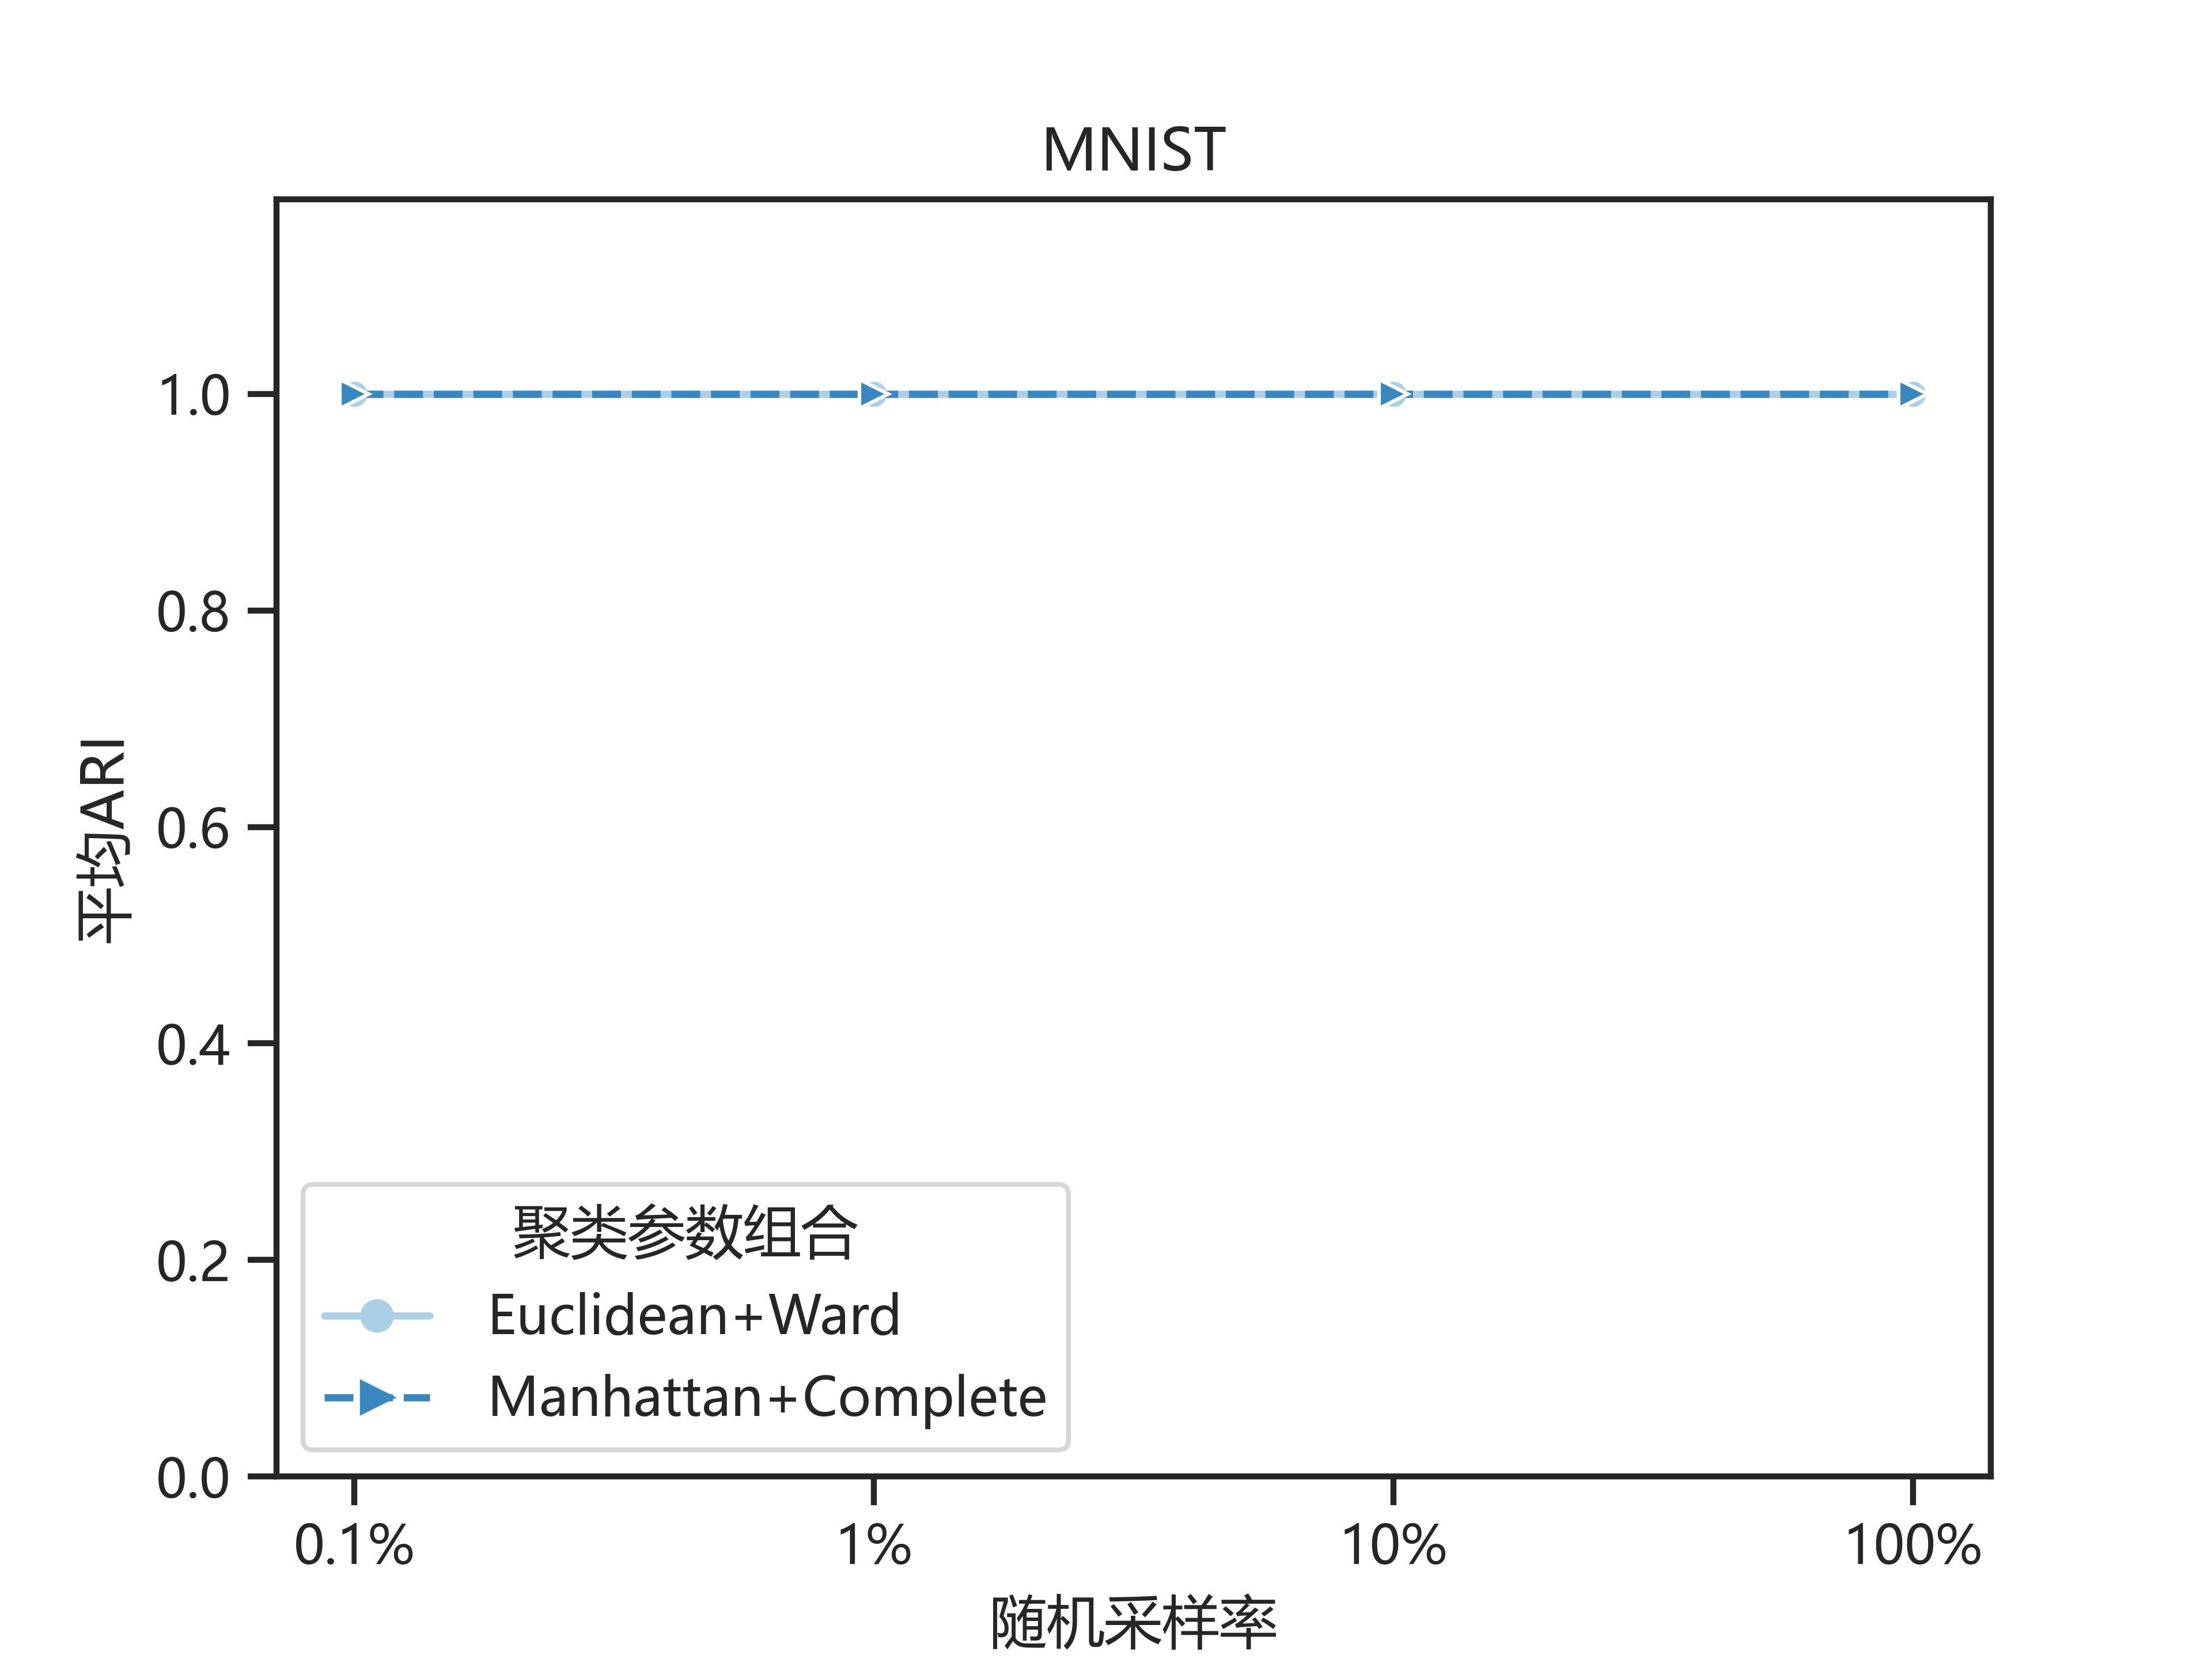
\includegraphics[scale=0.45]{figs/cmp-hcres-sf-re-win-mnist}
		\end{minipage}
	}
	\qquad
	\subfloat[CIFAR-10数据集平均ARI对比]{
		\begin{minipage}[b]{0.45\textwidth}
			\centering
			\label{hc-res-cmp:b}
			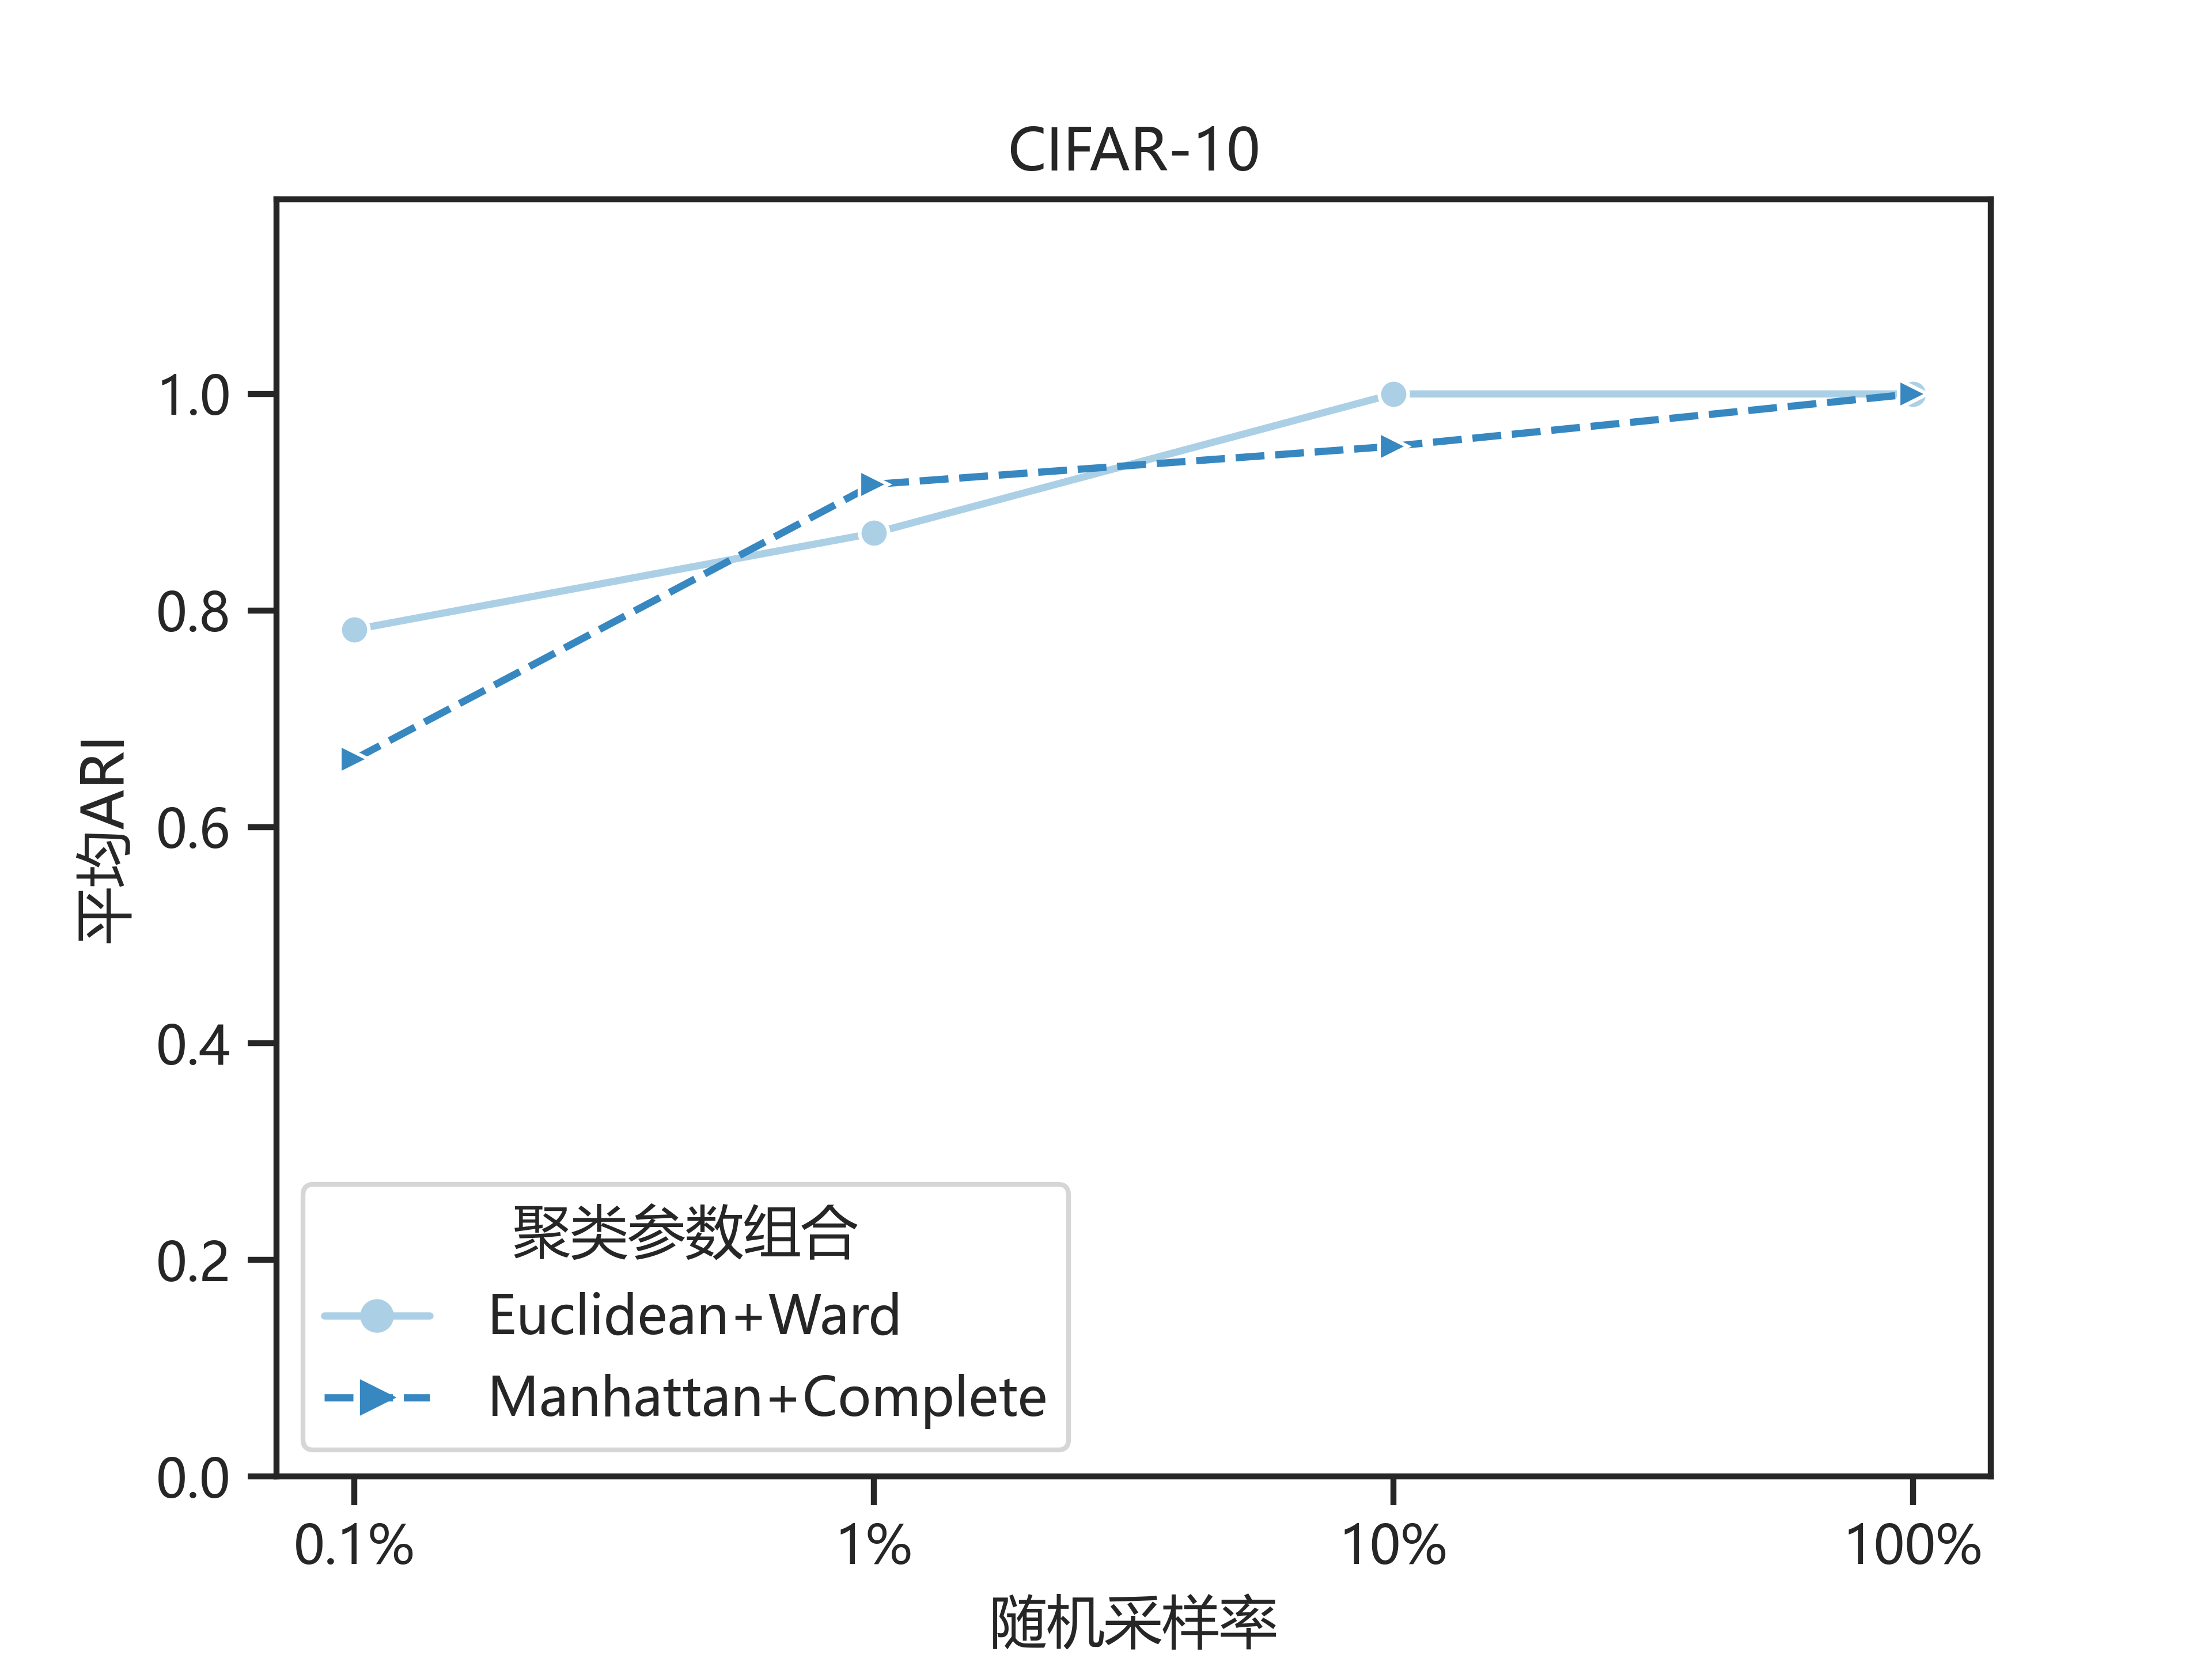
\includegraphics[scale=0.45]{figs/cmp-hcres-sf-re-win-cifar}
		\end{minipage}
	}
	\caption{不同参数组合聚类结果平均ARI对比}
	\label{hc-res-cmp}
\end{figure}
}

\subsubsection{效率测试}
PPFL+HC的性能瓶颈在于层次聚类过程中需要计算一次两两梯度间的距离,对于$n$个参与方,每个参与方梯度维度为$d$,其计算复杂度是 $O(n^2\times d)$。
于是本小节单独对距离矩阵的计算做了效率评估,包括对通信开销的评估和执行时间的评估。

\textbf{参与方数量的影响:}在图\ref{fig-cost:a}和图\ref{fig-cost:b}中,梯度的维度被固定为 $795$(采样率为1\%的MNIST模型参数维度),然后观察不同参与方数量对通信开销和执行时间的影响,发现随着参与方数量的增加,通信开销和执行时间都有比较大的增加,原因是参与方数量的增长,将导致计算和通信开销以平方级别增长。
考虑到聚类操作在训练过程中只进行一次,再结合梯度随机降维带来的效率提升,即使参与方数量增加也能将复杂度控制在可接受范围内。
其中对比不同的距离度量方式(欧式距离或者曼哈顿距离),从图中可以看到使用曼哈顿距离比使用欧式距离,在通信开销上有 8.93倍的提升,在执行时间上有 1.11-1.44倍的提升。SMD算法\ref{alg2}的性能优势来源于轻量的计算子模块,不涉及到开销更大的安全乘法操作。

\textbf{不同梯度维度的影响:}
直观的说,参与安全层次聚类的梯度维度越高,携带的特征越多,越容易被层次聚类划分到正确的类别。但是高维梯度给计算上带来了极大的开销,因此本小节探讨是否能通过裁剪部分梯度的维度,保证聚类精度损失可接受的同时,提升安全层次聚类的效率。
%为了减少安全距离矩阵计算的通信开销和执行时间开销,同时保证高的聚类精度,梯度将按照随机采样率在聚类前进行随机的降维操作。
在图\ref{fig-cost:c}和图\ref{fig-cost:d}中,逐步减少梯度的维度,同时比较聚类结果,结合表\ref{ari-sf-cmp}发现当梯度的随机采样率到1\%(MNIST梯度维度为795)时,保证了聚类精度的同时,最大限度的减小了计算和通信开销。梯度的维度较高,裁减了维度之后还能保持较好的特征,可以被层次聚类算法正确划分为不同类别。对比不同的距离度量方式,从图中可以看到曼哈顿距离对比欧式距离,在通信开销上有 4.78-8.93倍的提升,在执行时间上有1.33-1.77倍的提升。

综合效率测试和聚类指标测试,使用欧式距离或曼哈顿距离进行层次聚类时,聚类指标结果差异不大,但是在效率上曼哈顿距离优势明显,因此更推荐使用曼哈顿距离作为安全层次聚类的距离度量方式。

% 效率测试
{\wuhao
\begin{figure}[htb]
	\centering
	\subfloat[参与方数量变化对通信开销的影响]{
		\begin{minipage}[b]{0.45\textwidth}
			\centering
			\label{fig-cost:a}
			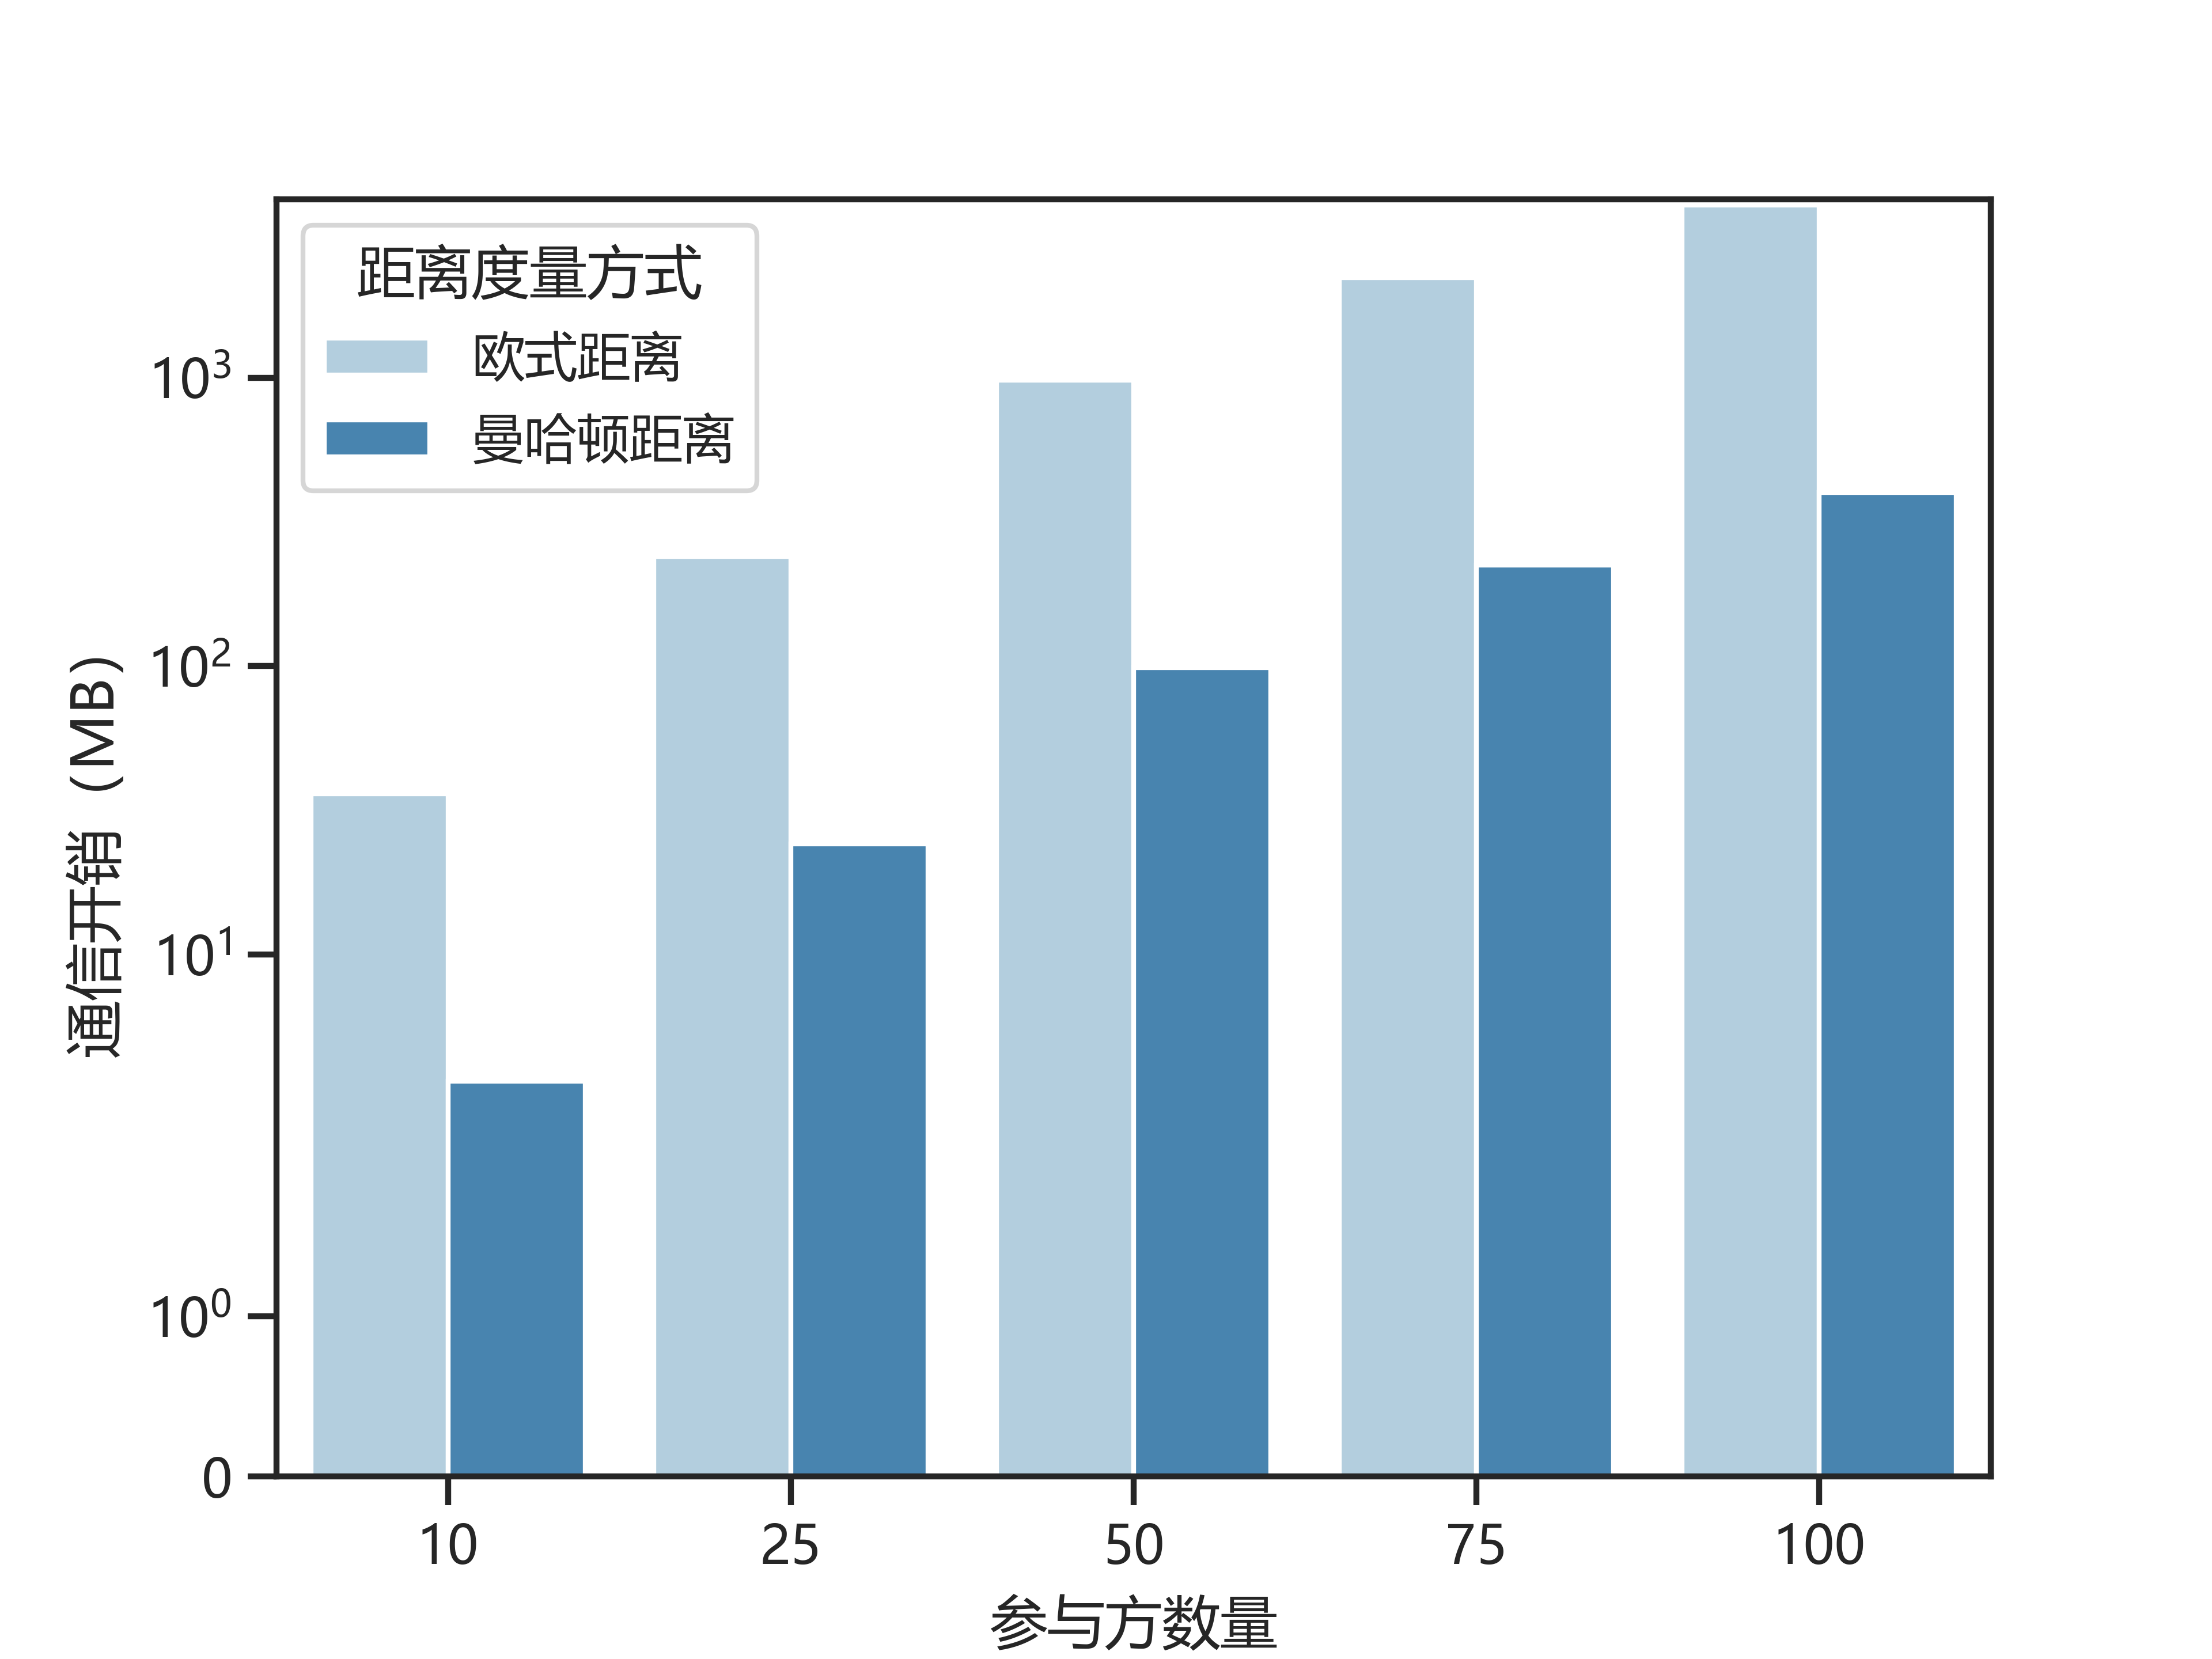
\includegraphics[scale=0.45]{figs/overheads/comm-win-party-795.png}
		\end{minipage}
	}
	% \hspace{-1.0in}
	\qquad
	\subfloat[参与方数量变化对执行时间的影响]{
		\begin{minipage}[b]{0.45\textwidth}
			\centering
			\label{fig-cost:b}
			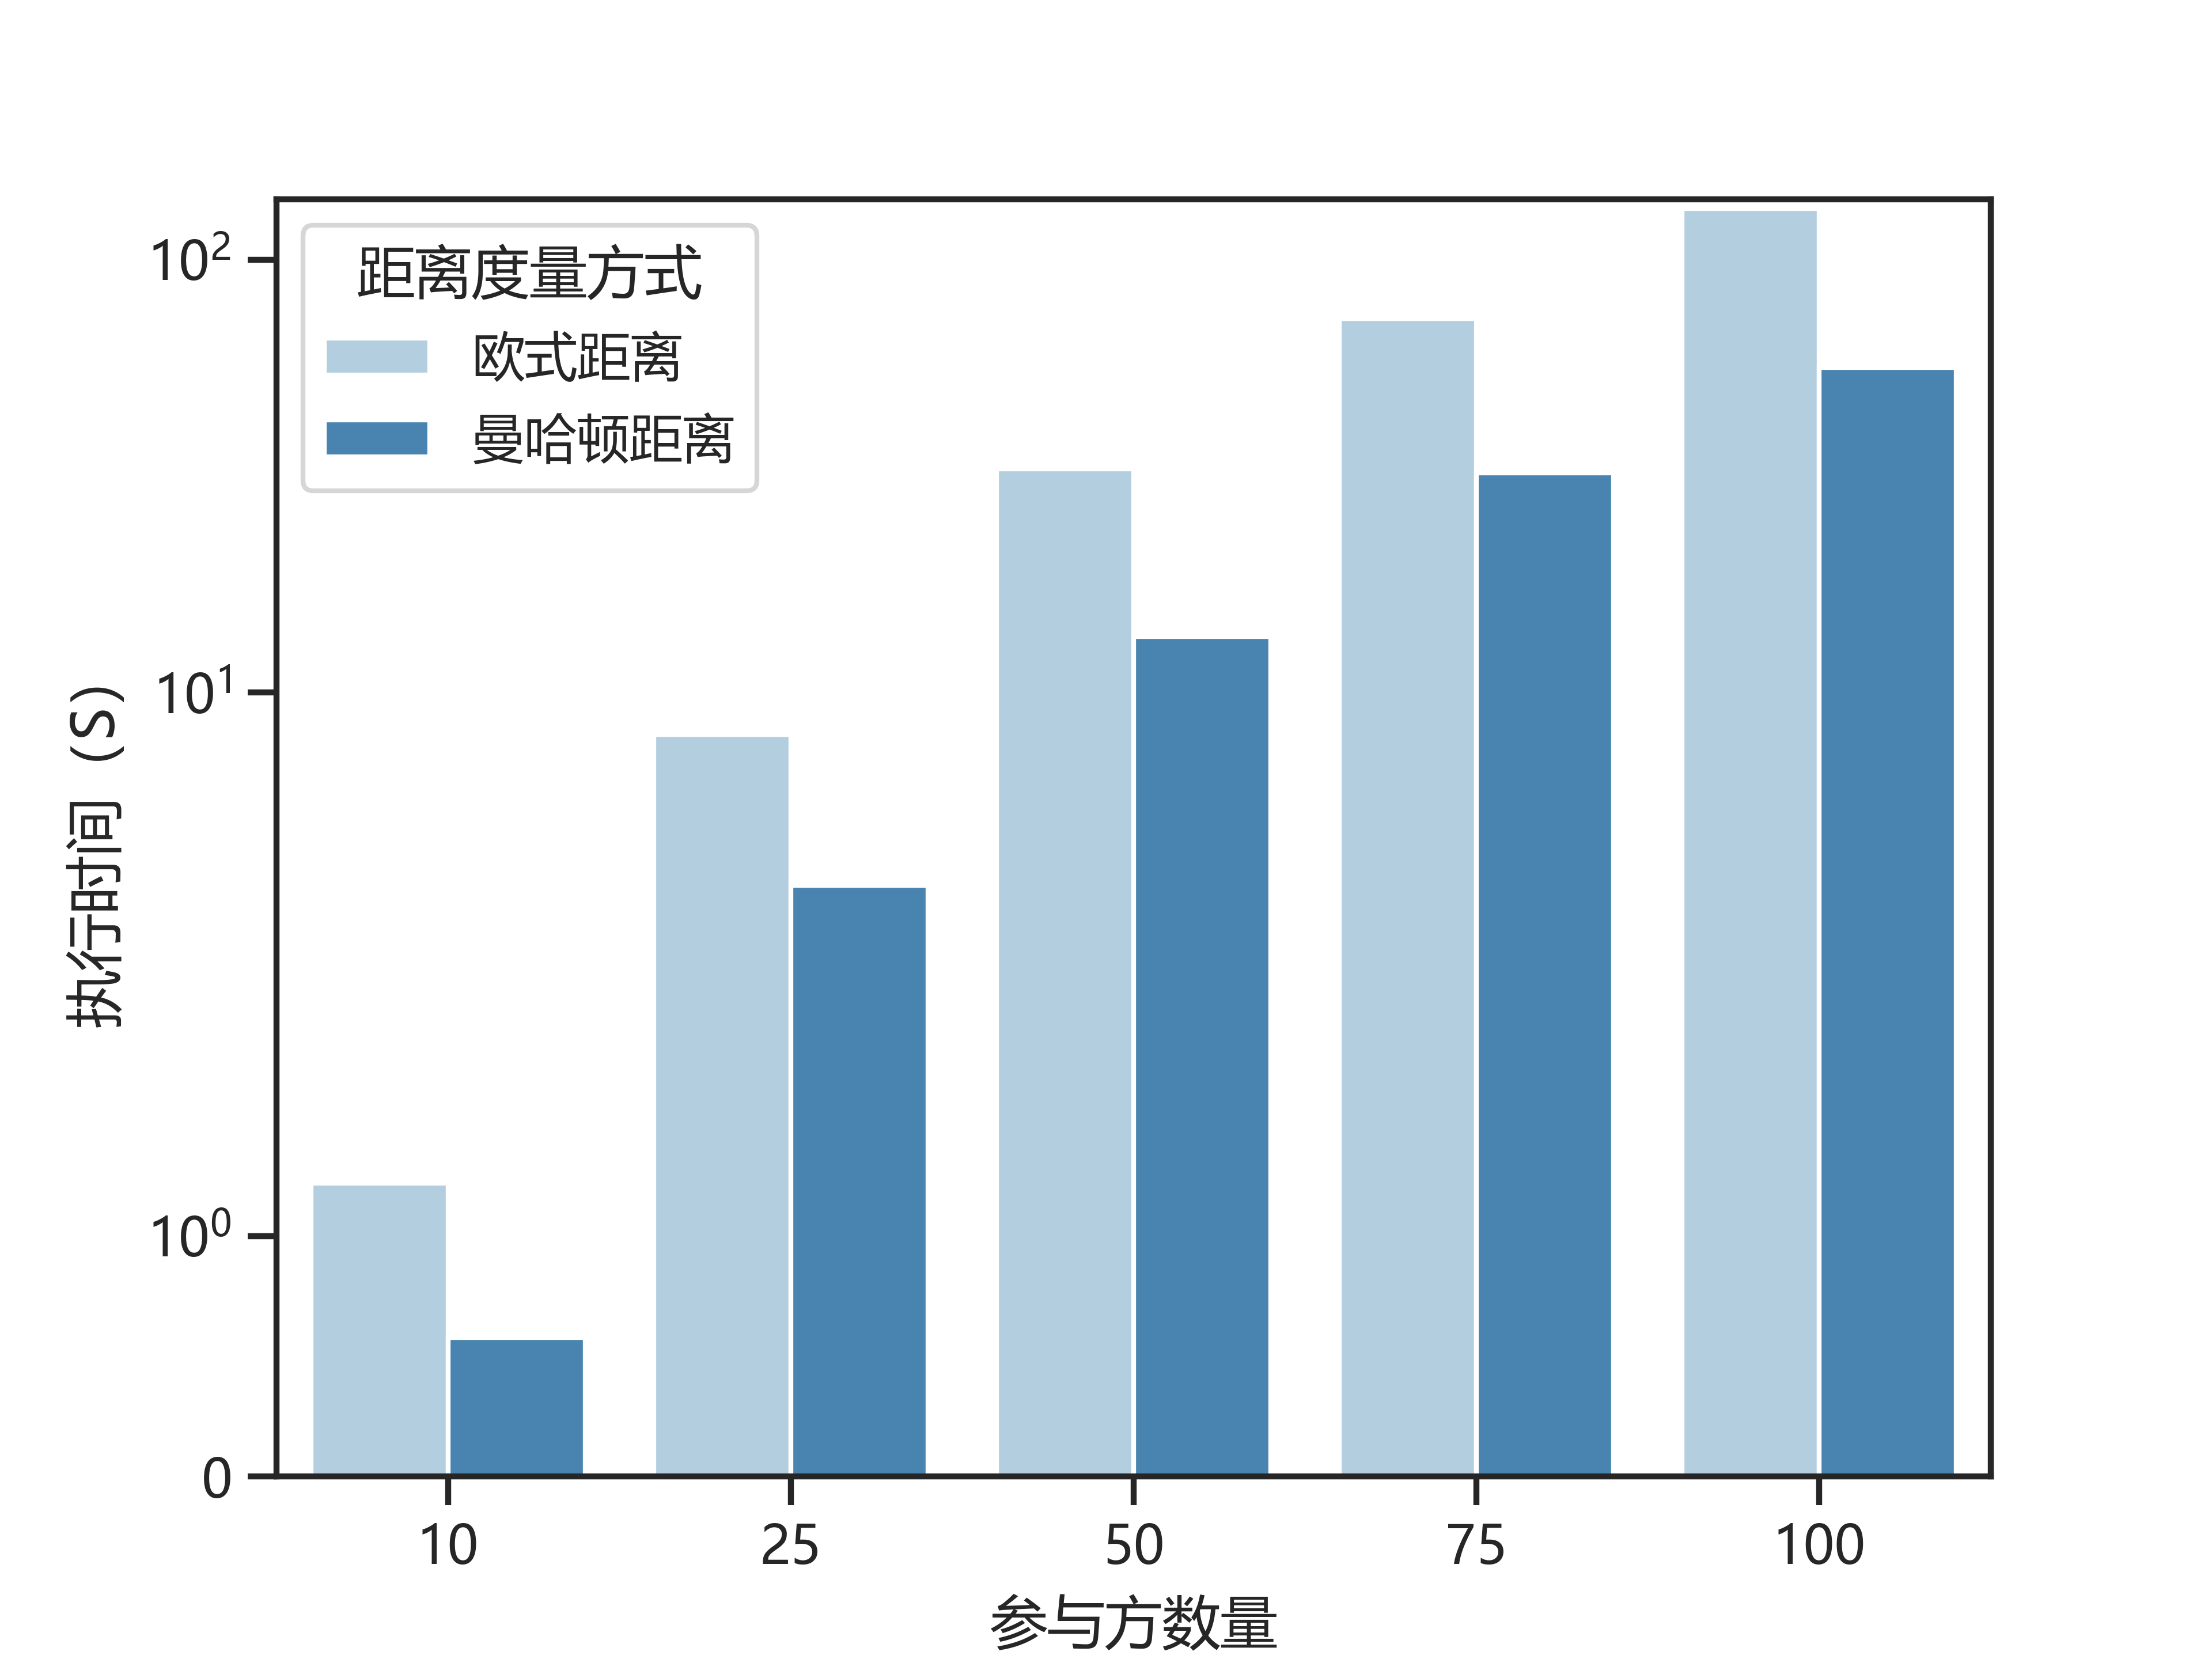
\includegraphics[scale=0.45]{figs/overheads/time-win-party-795.png}
		\end{minipage}
	}
	\qquad
	\subfloat[不同输入维度对通信开销的影响]{
		\begin{minipage}[b]{0.45\textwidth}
			\centering
			\label{fig-cost:c}
			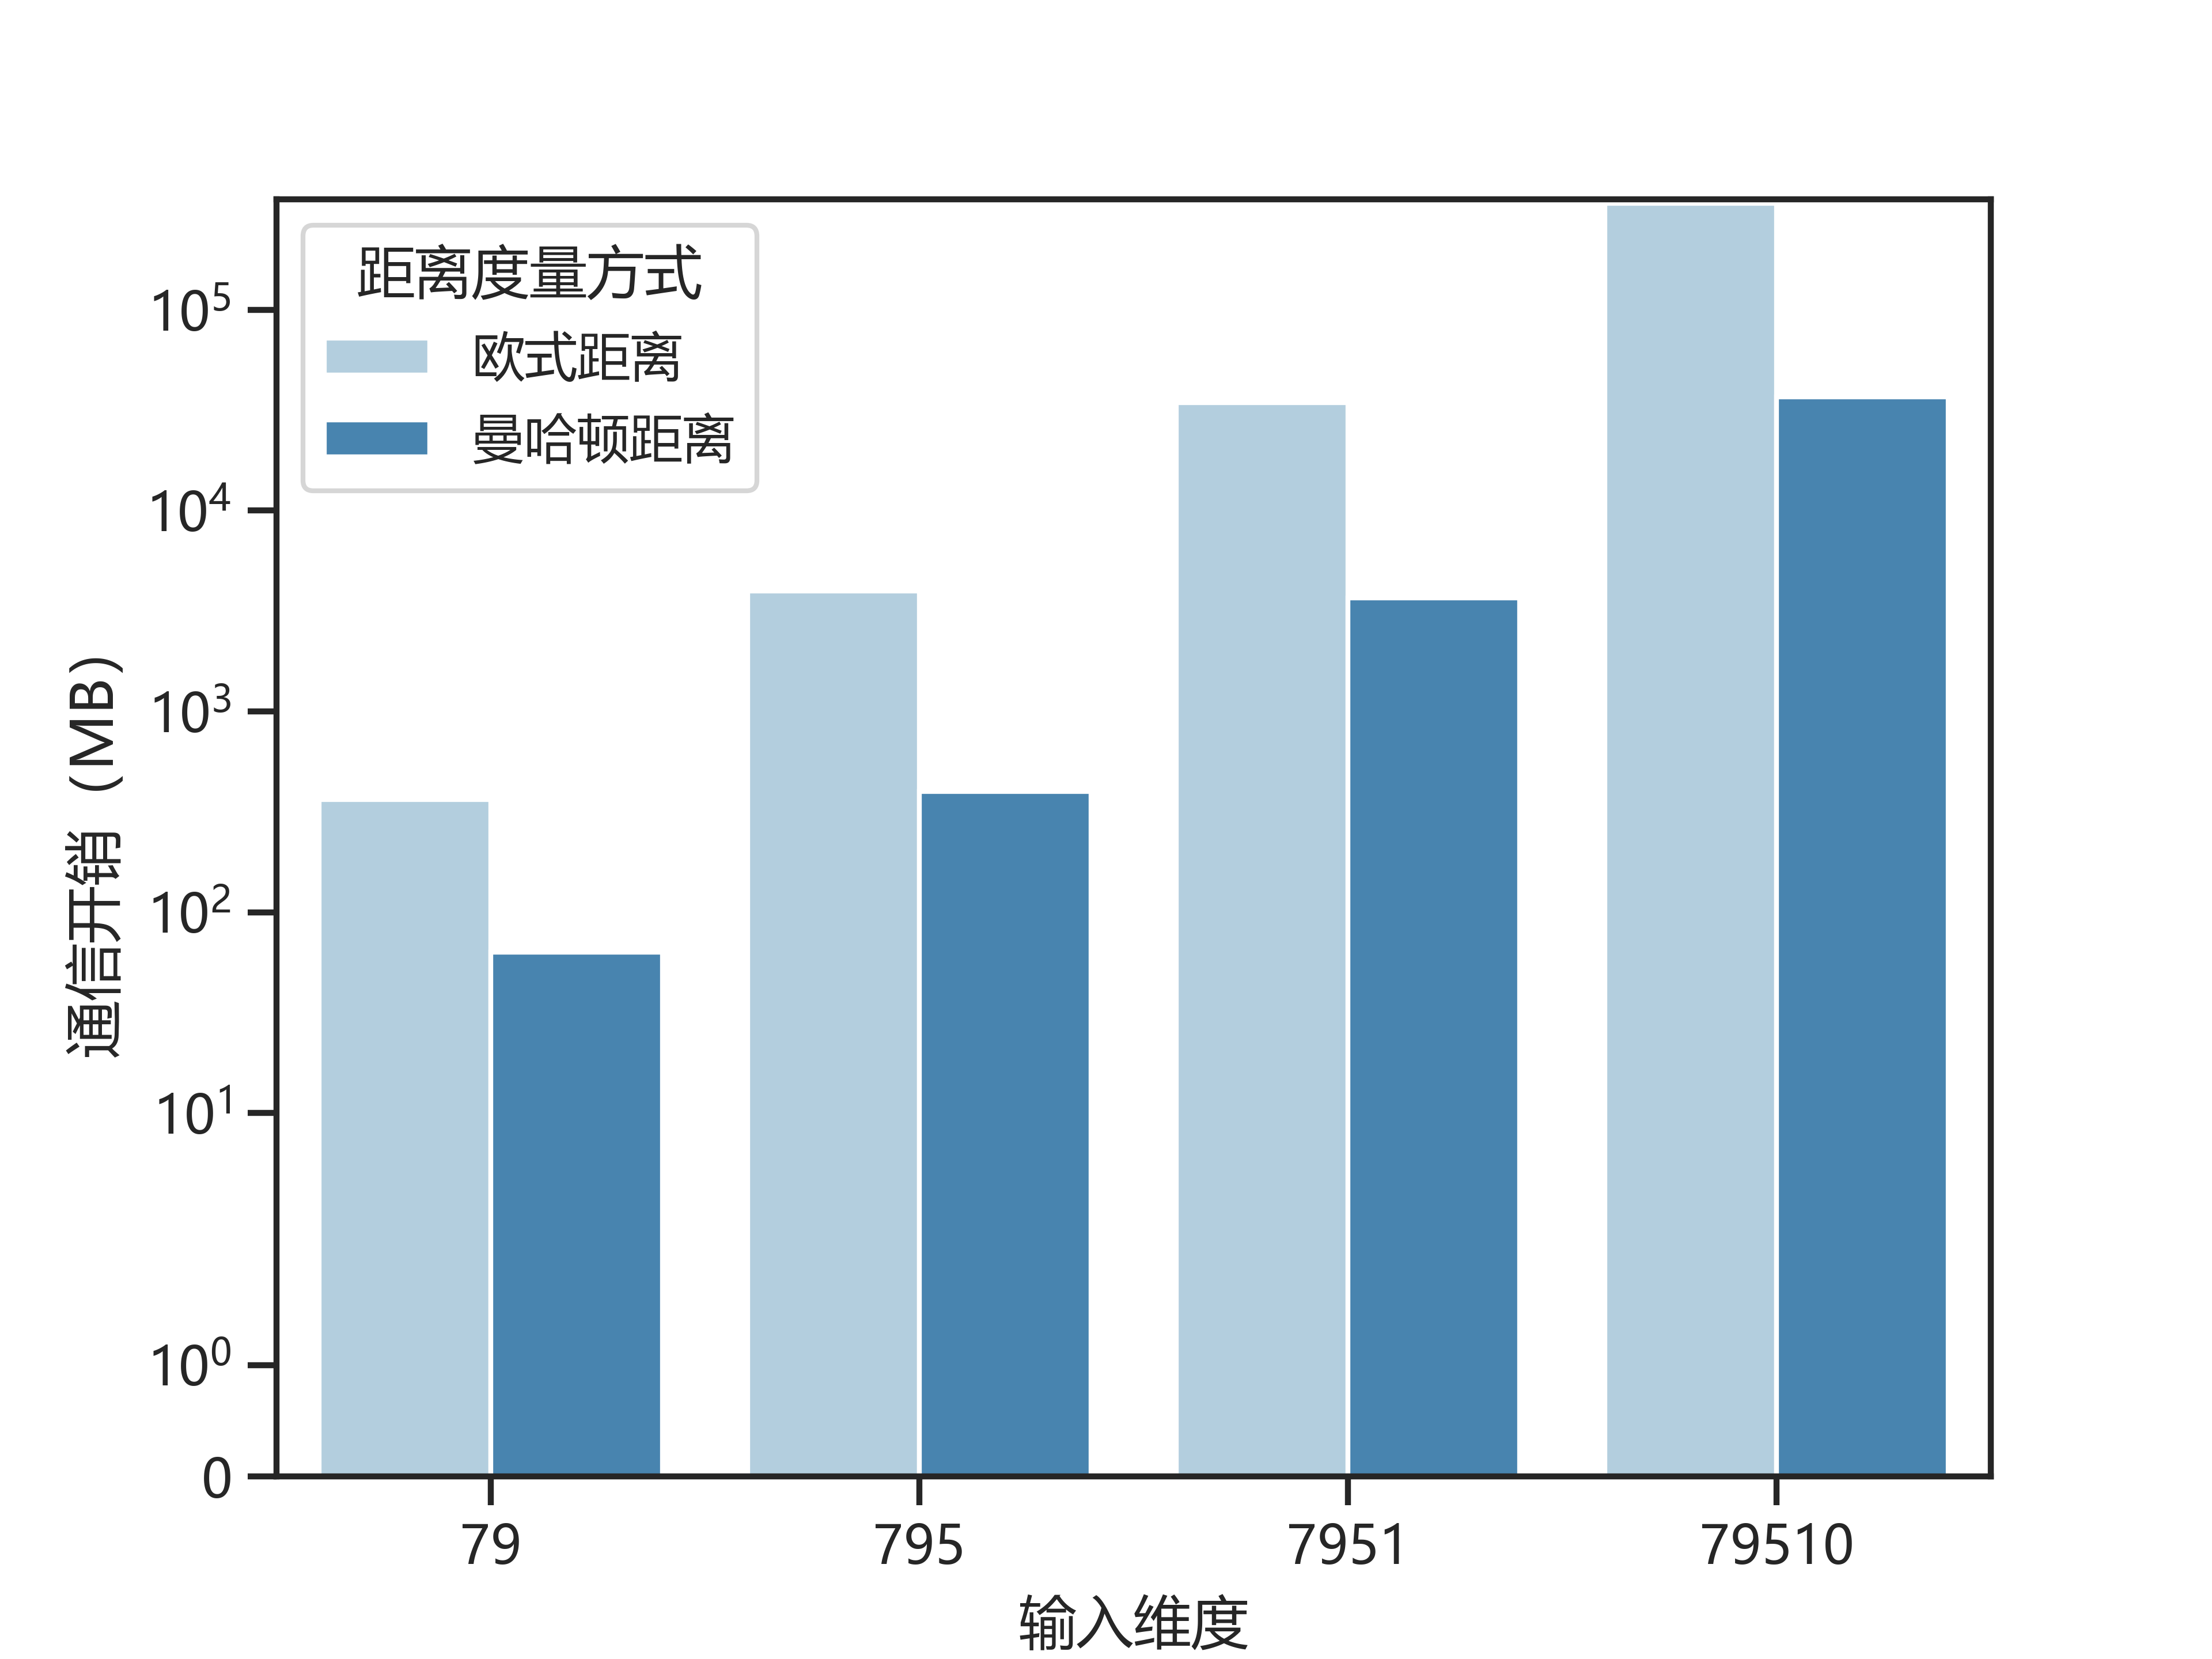
\includegraphics[scale=0.45]{figs/overheads/comm-win-dimension-100.png}
		\end{minipage}
	}
	\qquad
	\subfloat[不同输入维度对执行时间的影响]{
		\begin{minipage}[b]{0.45\textwidth}
			\centering
			\label{fig-cost:d}
			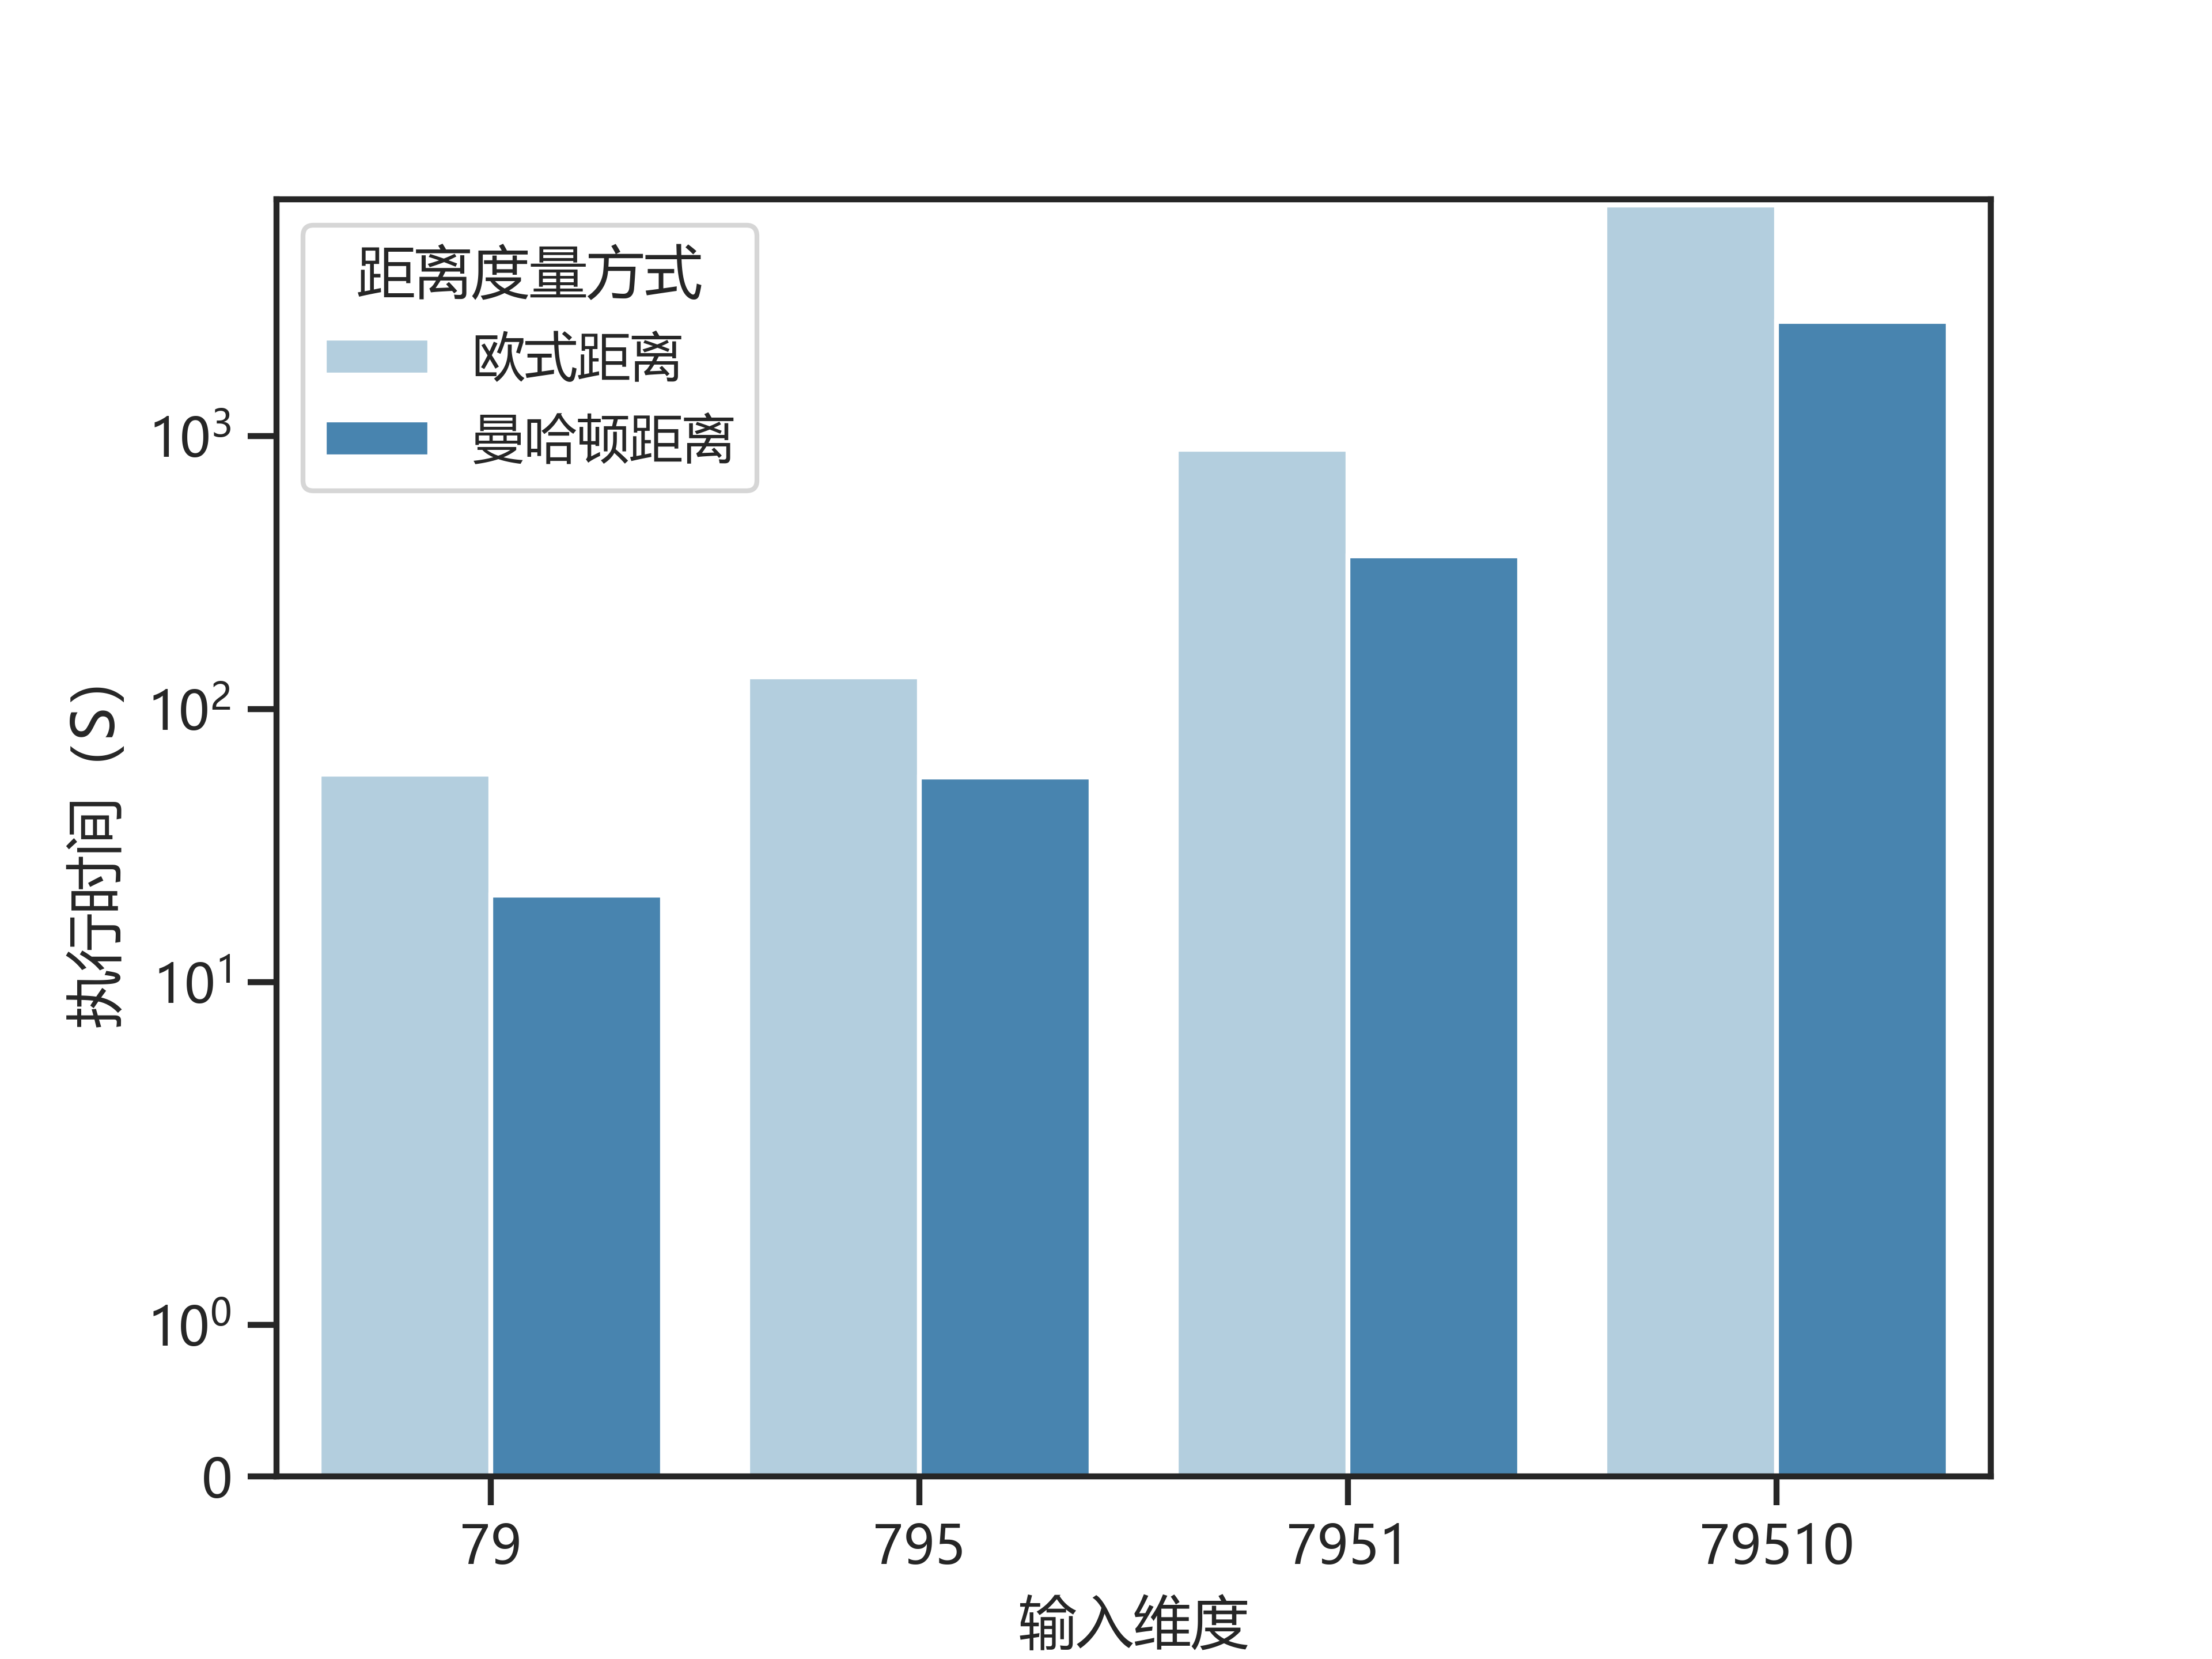
\includegraphics[scale=0.45]{figs/overheads/time-win-dimension-100.png}
		\end{minipage}
	}
	\caption[PPFL+HC效率评估]{不同的安全距离度量方式、不同参与方以及不同输入维度对本方案通信开销以及执行时间的影响,在图\ref{fig-cost:a} 与\ref{fig-cost:b}中,梯度维度固定为795,在图\ref{fig-cost:c}与\ref{fig-cost:d}中,参与方的数量被固定为100。}
	\label{fig-cost}
\end{figure}
}

\section{相关工作对比}\label{4-cmp}
表\ref{4-cmp2dp}展示了本章提出的方案PPFL+HC和基于DP的方案粗粒度上的对比。所对比的方案\cite{xiong2021privacy, noble2022differentially}都基于DP构建。
Xiong等人\cite{xiong2021privacy}提出了2DP-FL方案,它使用双DP的方式为本地模型和全局模型同时添加噪声。但是其提供的隐私保证较弱,更适用于算力较弱,需要对隐私保护做出妥协的物联网场景。
Noble等人\cite{noble2022differentially}使用DP改造SCAFFOLD,提出了DP-SCAFFOLD方案,致力于解决引入噪声带来的模型训练性能下降问题。以上方案妥协于数据可用性,只能提供一定程度上的隐私保护,无法实现对梯度的强隐私保护。同时此种类型的方案由于噪声的加入,不可避免的影响原始算法的性能。此外,对比PPFL+HC,2DP-FL与DP-SCAFFLOD的扩展性较弱,很难与其它基于训练算法的异质聚合方案结合。
\begin{table}[htbp] 	
	\centering 	
	\caption{与基于DP方案的粗粒度对比} 	
	\label{4-cmp2dp} 	
	\begin{tabular}{l|cccc} 		
		\toprule 		方案     & 隐私保护能力 & 维持原始算法性能 & 扩展性 & 算力要求 \\ 
		\midrule 		2DP+FL\cite{xiong2021privacy} & \LEFTcircle          & \ding{55}        & \Circle   & \LEFTcircle    \\ 
				DP-SCAFFOLD\cite{noble2022differentially} & \LEFTcircle          & \ding{55}        & \LEFTcircle   & \LEFTcircle    \\ 		
				本方案(PPFL+HC)    & \CIRCLE          & \ding{51}       & \CIRCLE   & \CIRCLE \\ 		
				\bottomrule 	
			\end{tabular} 
\end{table}

%\newpage
\section{本章小结}\label{4-conclusion}
本章提出了一个兼顾模型参数隐私保护和异质分布数据处理能力的联邦学习方案(PPFL+HC),在保证参与方本地梯度隐私和全局梯度隐私的前提下,实现了较高的异质分布数据联合训练准确率。PPFL+HC由高效的基于秘密共享的安全计算模块构成,其中包括SED、SMD、SHC和SGB等2PC协议。除此之外,在真实数据集上对两种极端的异质分布数据进行的实验,证明了PPFL+HC在保证隐私的同时提升了异质分布数据联合训练的准确率。

PPFL+HC对异质分布数据的性能提升源自于FL+HC\cite{briggs2020federated},因此也继承了FL+HC的缺点,即层次聚类的结果对全局模型的影响较大。还有一个限制是本章的框架需要两个不共谋的服务器,要实现单服务器的安全层次聚类需要更加细致完备的安全计算协议,同时也会遇到更多的性能瓶颈。这些问题的解决可以作为未来的研究方向。